\documentclass[12pt,twoside]{report}

\newcommand\hmmax{0}
\newcommand\bmmax{0}

\newcommand{\reporttitle}{
Generating Session-Typed WebSocket Applications in TypeScript
}
\newcommand{\reportauthor}{Anson Miu}
\newcommand{\reporttype}{MEng Individual Project}
\newcommand{\supervisor}{Prof. Nobuko Yoshida}
\newcommand{\sndmarker}{Dr. Iain Phillips}
\newcommand{\cid}{your college-id number}

% include files that load packages and define macros
%%%%%%%%%%%%%%%%%%%%%%%%%%%%%%%%%%%%%%%%%
% University Assignment Title Page 
% LaTeX Template
% Version 1.0 (27/12/12)
%
% This template has been downloaded from:
% http://www.LaTeXTemplates.com
%
% Original author:
% WikiBooks (http://en.wikibooks.org/wiki/LaTeX/Title_Creation)
%
% License:
% CC BY-NC-SA 3.0 (http://creativecommons.org/licenses/by-nc-sa/3.0/)
% 
% Instructions for using this template:
% This title page is capable of being compiled as is. This is not useful for 
% including it in another document. To do this, you have two options: 
%
% 1) Copy/paste everything between \begin{document} and \end{document} 
% starting at \begin{titlepage} and paste this into another LaTeX file where you 
% want your title page.
% OR
% 2) Remove everything outside the \begin{titlepage} and \end{titlepage} and 
% move this file to the same directory as the LaTeX file you wish to add it to. 
% Then add \input{./title_page_1.tex} to your LaTeX file where you want your
% title page.
%
%----------------------------------------------------------------------------------------
%	PACKAGES AND OTHER DOCUMENT CONFIGURATIONS
%----------------------------------------------------------------------------------------
\usepackage{ifxetex}
\usepackage{textpos}
\usepackage[sort,comma]{natbib}
\usepackage{kpfonts}
\usepackage[a4paper,hmargin=2.8cm,vmargin=2.0cm,includeheadfoot]{geometry}
\usepackage{ifxetex}
\usepackage{stackengine}
\usepackage{tabularx,longtable,multirow,subfigure,caption}%hangcaption
\usepackage{fncylab} %formatting of labels
\usepackage{fancyhdr}
\usepackage{color}
\usepackage[tight,ugly]{units}
\usepackage{url}
\usepackage{float}
\usepackage[english]{babel}
\usepackage{amsmath}
\usepackage{graphicx}
\usepackage[colorinlistoftodos]{todonotes}
\usepackage{dsfont}
\usepackage{epstopdf} % automatically replace .eps with .pdf in graphics
\usepackage{backref}
\usepackage{array}
\usepackage{latexsym}
\usepackage{etoolbox}

\usepackage{enumerate} % for numbering with [a)] format 

\usepackage{multicol}
\usepackage{setspace}



\ifxetex
\usepackage{fontspec}
\setmainfont[Scale=.8]{OpenDyslexic-Regular}
\else
\usepackage[pdftex,pagebackref,hypertexnames=false,colorlinks]{hyperref} % provide links in pdf
\hypersetup{pdftitle={},
  pdfsubject={}, 
  pdfauthor={\reportauthor},
  pdfkeywords={}, 
  pdfstartview=FitH,
  pdfpagemode={UseOutlines},% None, FullScreen, UseOutlines
  bookmarksnumbered=true, bookmarksopen=true, colorlinks,
    citecolor=black,%
    filecolor=black,%
    linkcolor=black,%
    urlcolor=black}
\usepackage[all]{hypcap}
\fi

\usepackage{tcolorbox}

% various theorems
\usepackage{amsthm}
\theoremstyle{plain}
\newtheorem{lemma}{Lemma}
\newtheorem{theorem}{Theorem}

\theoremstyle{definition}
\newtheorem{definition}{Definition}

\newtheoremstyle{proof}% name
  {\topsep}% space above
  {\topsep}% space below
  {}% body font
  {}% indent amount
  {\itshape}% theorem head font
  {.}% punctuation after theorem head
  {.5em}% space after theorem head
  {\thmname{#1}\thmnumber{ #2}\thmnote{ (#3)}}% theorem head spec
\theoremstyle{proof}
\newtheorem*{remark}{Remark}
\newtheorem*{thmproof}{Proof}

% example-environment
\newenvironment{example}[1][]
{ 
\vspace{4mm}
\noindent\makebox[\linewidth]{\rule{\hsize}{1.5pt}}
\textbf{Example #1}\\
}
{ 
\noindent\newline\makebox[\linewidth]{\rule{\hsize}{1.0pt}}
}



%\renewcommand{\rmdefault}{pplx} % Palatino
% \renewcommand{\rmdefault}{put} % Utopia

\ifxetex
\else
\renewcommand*{\rmdefault}{bch} % Charter
\renewcommand*{\ttdefault}{cmtt} % Computer Modern Typewriter
%\renewcommand*{\rmdefault}{phv} % Helvetica
%\renewcommand*{\rmdefault}{iwona} % Avant Garde
\fi

\setlength{\parindent}{1em}  % indentation of paragraph


\setlength{\headheight}{14.5pt}
\pagestyle{fancy}
\fancyfoot[ER,OL]{\thepage}%Page no. in the left on
                                %odd pages and on right on even pages
\fancyfoot[OC,EC]{\sffamily }
\renewcommand{\headrulewidth}{0.1pt}
\renewcommand{\footrulewidth}{0.1pt}
\captionsetup{margin=10pt,font=small,labelfont=bf}


%--- chapter heading

\def\@makechapterhead#1{%
  \vspace*{10\p@}%
  {\parindent \z@ \raggedright %\sffamily
        %{\Large \MakeUppercase{\@chapapp} \space \thechapter}
        %\\
        %\hrulefill
        %\par\nobreak
        %\vskip 10\p@
    \interlinepenalty\@M
    \Huge \bfseries 
    \thechapter \space\space #1\par\nobreak
    \vskip 30\p@
  }}

%---chapter heading for \chapter*  
\def\@makeschapterhead#1{%
  \vspace*{10\p@}%
  {\parindent \z@ \raggedright
    \sffamily
    \interlinepenalty\@M
    \Huge \bfseries  
    #1\par\nobreak
    \vskip 30\p@
  }}
  



% %%%%%%%%%%%%% boxit
\def\Beginboxit
   {\par
    \vbox\bgroup
	   \hrule
	   \hbox\bgroup
		  \vrule \kern1.2pt %
		  \vbox\bgroup\kern1.2pt
   }

\def\Endboxit{%
			      \kern1.2pt
		       \egroup
		  \kern1.2pt\vrule
		\egroup
	   \hrule
	 \egroup
   }	

\newenvironment{boxit}{\Beginboxit}{\Endboxit}
\newenvironment{boxit*}{\Beginboxit\hbox to\hsize{}}{\Endboxit}



\allowdisplaybreaks

\makeatletter
\newcounter{elimination@steps}
\newcolumntype{R}[1]{>{\raggedleft\arraybackslash$}p{#1}<{$}}
\def\elimination@num@rights{}
\def\elimination@num@variables{}
\def\elimination@col@width{}
\newenvironment{elimination}[4][0]
{
    \setcounter{elimination@steps}{0}
    \def\elimination@num@rights{#1}
    \def\elimination@num@variables{#2}
    \def\elimination@col@width{#3}
    \renewcommand{\arraystretch}{#4}
    \start@align\@ne\st@rredtrue\m@ne
}
{
    \endalign
    \ignorespacesafterend
}
\newcommand{\eliminationstep}[2]
{
    \ifnum\value{elimination@steps}>0\leadsto\quad\fi
    \left[
        \ifnum\elimination@num@rights>0
            \begin{array}
            {@{}*{\elimination@num@variables}{R{\elimination@col@width}}
            |@{}*{\elimination@num@rights}{R{\elimination@col@width}}}
        \else
            \begin{array}
            {@{}*{\elimination@num@variables}{R{\elimination@col@width}}}
        \fi
            #1
        \end{array}
    \right]
    & 
    \begin{array}{l}
        #2
    \end{array}
    &%                                    moved second & here
    \addtocounter{elimination@steps}{1}
}
\makeatother

%% Fast macro for column vectors
\makeatletter  
\def\colvec#1{\expandafter\colvec@i#1,,,,,,,,,\@nil}
\def\colvec@i#1,#2,#3,#4,#5,#6,#7,#8,#9\@nil{% 
  \ifx$#2$ \begin{bmatrix}#1\end{bmatrix} \else
    \ifx$#3$ \begin{bmatrix}#1\\#2\end{bmatrix} \else
      \ifx$#4$ \begin{bmatrix}#1\\#2\\#3\end{bmatrix}\else
        \ifx$#5$ \begin{bmatrix}#1\\#2\\#3\\#4\end{bmatrix}\else
          \ifx$#6$ \begin{bmatrix}#1\\#2\\#3\\#4\\#5\end{bmatrix}\else
            \ifx$#7$ \begin{bmatrix}#1\\#2\\#3\\#4\\#5\\#6\end{bmatrix}\else
              \ifx$#8$ \begin{bmatrix}#1\\#2\\#3\\#4\\#5\\#6\\#7\end{bmatrix}\else
                 \PackageError{Column Vector}{The vector you tried to write is too big, use bmatrix instead}{Try using the bmatrix environment}
              \fi
            \fi
          \fi
        \fi
      \fi
    \fi
  \fi 
}  
\makeatother

\robustify{\colvec}

%%% Local Variables: 
%%% mode: latex
%%% TeX-master: "notes"
%%% End: 
 % various packages needed for maths etc.
% quick way of adding a figure
\newcommand{\fig}[3]{
 \begin{center}
 \scalebox{#3}{\includegraphics[#2]{#1}}
 \end{center}
}

%\newcommand*{\point}[1]{\vec{\mkern0mu#1}}
\newcommand{\ci}[0]{\perp\!\!\!\!\!\perp} % conditional independence
\newcommand{\point}[1]{{#1}} % points 
% \renewcommand{\vec}[1]{{\boldsymbol{{#1}}}} % vector
\newcommand{\mat}[1]{{\boldsymbol{{#1}}}} % matrix
\newcommand{\R}[0]{\mathds{R}} % real numbers
\newcommand{\Z}[0]{\mathds{Z}} % integers
\newcommand{\N}[0]{\mathds{N}} % natural numbers
\newcommand{\nat}[0]{\mathds{N}} % natural numbers
\newcommand{\Q}[0]{\mathds{Q}} % rational numbers
\ifxetex
\newcommand{\C}[0]{\mathds{C}} % complex numbers
\else
\newcommand{\C}[0]{\mathds{C}} % complex numbers
\fi
\newcommand{\tr}[0]{\text{tr}} % trace
\renewcommand{\d}[0]{\mathrm{d}} % total derivative
\newcommand{\inv}{^{-1}} % inverse
\newcommand{\id}{\mathrm{id}} % identity mapping
\renewcommand{\dim}{\mathrm{dim}} % dimension
\newcommand{\rank}[0]{\mathrm{rk}} % rank
\newcommand{\determ}[1]{\mathrm{det}(#1)} % determinant
\newcommand{\scp}[2]{\langle #1 , #2 \rangle}
\newcommand{\kernel}[0]{\mathrm{ker}} % kernel/nullspace
\newcommand{\img}[0]{\mathrm{Im}} % image
\newcommand{\idx}[1]{{(#1)}}
\DeclareMathOperator*{\diag}{diag}
\newcommand{\E}{\mathds{E}} % expectation
\newcommand{\var}{\mathds{V}} % variance
\newcommand{\gauss}[2]{\mathcal{N}\big(#1,\,#2\big)} % gaussian distribution N(.,.)
\newcommand{\gaussx}[3]{\mathcal{N}\big(#1\,|\,#2,\,#3\big)} % gaussian distribution N(.|.,.)
\newcommand{\gaussBig}[2]{\mathcal{N}\left(#1,\,#2\right)} % see above, but with brackets that adjust to the height of the arguments
\newcommand{\gaussxBig}[3]{\mathcal{N}\left(#1\,|\,#2,\,#3\right)} % see above, but with brackets that adjust to the height of the arguments
\DeclareMathOperator{\cov}{Cov} % covariance (matrix) 
\ifxetex
\renewcommand{\T}[0]{^\top} % transpose
\else
\newcommand{\T}[0]{^\top}
\fi
% matrix determinant
\newcommand{\matdet}[1]{
\left|
\begin{matrix}
#1
\end{matrix}
\right|
}



%%% various color definitions
\definecolor{darkgreen}{rgb}{0,0.6,0}

\newcommand{\blue}[1]{{\color{blue}#1}}
\newcommand{\red}[1]{{\color{red}#1}}
\newcommand{\green}[1]{{\color{darkgreen}#1}}
\newcommand{\orange}[1]{{\color{orange}#1}}
\newcommand{\magenta}[1]{{\color{magenta}#1}}
\newcommand{\cyan}[1]{{\color{cyan}#1}}


% redefine emph
\renewcommand{\emph}[1]{\blue{\bf{#1}}}

% place a colored box around a character
\gdef\colchar#1#2{%
  \tikz[baseline]{%
  \node[anchor=base,inner sep=2pt,outer sep=0pt,fill = #2!20] {#1};
    }%
}%

%%%%%%%%%%%%%%%%%%%%%%%%%%%%%%%

\usepackage{ bm }					% \bm
\usepackage{ cmll }				% \with
\usepackage{ mathtools }		% \mathmakebox

% GENERAL
\newcommand{\role}[1]{
{\color{blue}\bm{\mathsf{#1}}}
}
\newcommand{\mrole}[1]{
{\mathtt{#1}}
}
\newcommand{\mroles}[2]{
{\mrole{#1}\mrole{#2}}
}
\newcommand{\pt}[1]{
{\textnormal{\texttt{pt}}\left({#1}\right)}
}
\newcommand{\rulename}[1]{
[\textsc{#1}]
}
\newcommand{\hlrulename}[1]{
\hl{[\textsc{#1}]}
}
\newcommand{\projconf}[1]{
{\left\langle{#1}\right\rangle}
}
\newcommand{\subtype}{
\prec
}

% NEW GENERAL
\newcommand{\centroidop}{\circledast}
\newcommand{\centroid}[2]{
{#1} \centroidop \mrole{#2}
}

% GLOBAL TYPES
\newcommand{\tend}{\textnormal{\texttt{end}}}
\newcommand{\trecvar}{\textnormal{\texttt{t}}}
\newcommand{\trec}[1]{\mu\trecvar.{#1}}
\newcommand{\gcommone}[3]{
\mrole{#1} \to \mrole{#2}. ~ {#3} :
}
\newcommand{\gcomm}[4]{
\mrole{#1} \to \mrole{#2} : \left\{ {#3} \right\}_{#4}
}
\newcommand{\gtrans}[5]{
\mrole{#1} \rightsquigarrow \mrole{#2}. ~ {#3} : \left\{ {#4} \right\}_{#5}
}
\newcommand{\wf}[1]{
\textnormal{\texttt{wellFormed}}\left(#1\right)
}
\newcommand{\proj}[2]{
{#1} \projop \mrole{#2}
}
\newcommand{\projop}{\upharpoonright}
\newcommand{\mergeop}{
\sqcap
}
\newcommand{\MERGEOP}{
{\mbox{\LARGE$\sqcap$}}
}
\newcommand{\tmerge}[2]{
{#1}\,{\mergeop}\,{#2}
}

% NEW GLOBAL TYPES
\newcommand{\grouteone}[4]{
\mrole{#1} \xrightarrow[\mrole{#3}]{} \mrole{#2}. ~ {#4} :
}
\newcommand{\groute}[5]{
\mrole{#1} \xrightarrow[\mrole{#3}]{} \mrole{#2} : \left\{ {#4} \right\}_{#5}
}
\newcommand{\gtransroute}[6]{
\mrole{#1} \underset{\mrole{#3}}{\rightsquigarrow} \mrole{#2}. ~ {#4} : \left\{ {#5} \right\}_{#6}
}
\newcommand{\wfnew}[2]{
\textnormal{\texttt{wellFormed}}\left(#1, \mrole{#2}\right)
}

% LOCAL TYPES
\newcommand{\tbra}[3]{
\mrole{#1} \with \left\{ #2 \right\}_{#3}
}
\newcommand{\tsel}[3]{
\mrole{#1} \oplus \left\{ {#2} \right\}_{#3}
}
\newcommand{\tselone}[2]{
\mrole{#1} \oplus {#2}
}
\newcommand{\lty}[1]{
T_{\mrole{#1}}
}
\newcommand{\pinP}{
{\mrole{p} \in \mathcal{P}}
}
\newcommand{\qqinP}{
{\mroles{q}{q'} \in \mathcal{P}}
}

% NEW LOCAL TYPES
\newcommand{\router}[4]{
\left(\mrole{#1} \hookrightarrow \mrole{#2}: \left\{{#3}\right\}_{#4}\right)
}
\newcommand{\routerone}[4]{
\texttt{route}\left(\mrole{#1} \hookrightarrow \mrole{#2}: {#3}.~{#4}\right)
}
\newcommand{\routertrans}[5]{
\left(\mrole{#1} \looparrowright \mrole{#2}. ~ {#3} : \left\{{#4}\right\}_{#5}\right)
}

\newcommand{\tselproxy}[4]{
\tsel{\mrole{#1}_{\mrole{#2}}}{#3}{#4}
}

\newcommand{\tbraproxy}[4]{
\tbra{\mrole{#1}_{\mrole{#2}}}{#3}{#4}
}

% LTS
\newcommand{\aout}[3]{
\mrole{#1}\mrole{#2}!{#3}
}
\newcommand{\ain}[3]{
\mrole{#1}\mrole{#2}?{#3}
}
\newcommand{\subj}[1]{
\text{subj}({#1})
}
\newcommand{\treduce}[3]{
{#1} \xrightarrow{\mathmakebox[1em]{#3}} {#2} 
}
\newcommand{\treducelong}[3]{
{#1} \xrightarrow{\mathmakebox[3.5em]{#3}} {#2} 
}

% NEW LTS
\newcommand{\via}[2]{
{\texttt{via}_{\mrole{#1}}({#2})}
} % short-hand notation and macros

\usepackage[nottoc]{tocbibind}
\setcitestyle{numbers}
	
% Change table/figure counter
\usepackage{chngcntr}

% Highlighting
\usepackage{soul}

% Graphics path
\graphicspath{ {figures/} }

\usepackage{underscore}

\usepackage{listings}

% Fancy names
\newcommand{\fancyname}[1]{\textsc{#1}}
\newcommand{\trole}[1]{\texttt{#1}}
\newcommand{\tmsg}[1]{\texttt{#1}}
\newcommand{\tprotocol}[1]{\textsc{#1}}

% Nicer references
\usepackage[noabbrev, capitalise]{cleveref}

% Font?
%\usepackage{ascii}
%\usepackage[T1]{fontenc}
%\renewcommand\ttfamily{\asciifamily}


% Includes

% Proof trees
%\usepackage{amsthm}
%\theoremstyle{plain}
%
%\newtheorem{thm}{Theorem}[section]
%\newtheorem{cor}{Corollary}[theorem]
%\newtheorem{lem}[theorem]{Lemma}
%\usepackage{proof}
\usepackage{bussproofs}

% Code listing

\lstdefinelanguage{Scribble}{
  keywords={module, type, from, as, global,protocol, role, to, choice, at, or, do},
  keywordstyle=\color{blue}\bfseries,
  identifierstyle=\color{black},
  sensitive=false,
  comment=[l]{//},
  morecomment=[s]{/*}{*/},
  commentstyle=\color{darkgray}\ttfamily,
  stringstyle=\color{purple}\ttfamily,
  morestring=[b]',
  morestring=[b]"
}
\lstdefinelanguage{JavaScript}{
  keywords={typeof, new, true, false, catch, function, return, null, catch, switch, var, if, in, while, do, else, case, break, class, export, boolean, throw, implements, import, this, const, let, extends, async, await, namespace, type, abstract, any, number, string, instanceof, typeof, declare, never,enum,constructor,public,private,void,super,undefined},
  keywordstyle=\color{blue}\bfseries,
%  ndkeywords={class, export, boolean, throw, implements, import, this},
%  ndkeywordstyle=\color{darkgray}\bfseries,
  identifierstyle=\color{black},
  sensitive=true,
  comment=[l]{//},
  morecomment=[s]{/*}{*/},
  commentstyle=\color{darkgray}\ttfamily,
  stringstyle=\color{purple}\ttfamily,
  morestring=[b]',
  morestring=[b]"
}
\lstdefinelanguage{Python}{
  keywords={class, self, def, cls, int, str, bool, pass, return, from, import, and, if, else, None, is, not},
  keywordstyle=\color{blue}\bfseries,
  identifierstyle=\color{black},
  comment=[l]{\#},
  commentstyle=\color{darkgray}\ttfamily,
  stringstyle=\color{purple}\ttfamily,
  morestring=[b]',
  morestring=[b]"
}
\lstset{
	basicstyle=\footnotesize\ttfamily,
	numberstyle=\tiny\ttfamily,
	numbers=left,
	frame=single,
	tabsize=4,
    xleftmargin=1.25em,
    framexrightmargin=-0.25em,
    escapeinside={(*@}{@*)}
}
\def\lstonelinejs{\lstinline[language=javascript,basicstyle=\ttfamily]}

% Figure and table counter
\usepackage{chngcntr}
\counterwithout{figure}{chapter}
\counterwithout{table}{chapter}

% Commands
%\newcommand{\term}[1]{\textit{#1}}
%\newcommand{\mathref}[1]{\textsection #1}
%
%\newcommand{\rulename}[1]{[\textsc{#1}]}
%
%\newcommand{\piin}[2]{#1(#2)}
%\newcommand{\piout}[2]{\bar{#1}\langle #2 \rangle }
%\newcommand{\parti}[1]{{\color{blue}\mathbf{#1}}}
%
%\newcommand{\send}[2]{#1!\langle #2 \rangle}
%\newcommand{\recv}[2]{#1?(#2)}
%\newcommand{\bra}[2]{#1 \rhd \left\{#2\right\}}
%\newcommand{\sel}[3]{#1 \lhd #2 \langle #3 \rangle}
%
%\newcommand{\tysend}[2]{#1![#2]}
%\newcommand{\tyrecv}[2]{#1?[#2]}
%\newcommand{\tybra}[2]{#1 \& \left\{#2\right\}}
%\newcommand{\tysel}[2]{#1 \oplus \left\{#2\right\}}


% Typewriter font
% \renewcommand{\ttdefault}{pcr} % selects Courier font

% Citation style
\setcitestyle{square}

%% PROOF TREES

% CODE LISTING

% COMMANDS
\usepackage{ wasysym }
\usepackage{ amssymb }
\usepackage{ xcolor }
\usepackage{ bm }
\usepackage{ cmll }
\usepackage{ array } 
\usepackage{ mathtools }
\usepackage{ stmaryrd } 

%% TEXT
\newcommand{\rulename}[1]{
[\textsc{#1}]
}

%% SYMBOLS
\newcommand{\role}[1]{
{\color{blue}\bm{\mathsf{#1}}}
}

%% PI CALCULUS
\newcommand{\nil}{
\mathbf{0}
}
\newcommand{\piin}[2]{
{#1}({#2})
}
\newcommand{\piout}[2]{
\bar{#1}\langle {#2} \rangle
}
\newcommand{\pipar}[2]{
\left({#1}\mid{#2}\right)
}
\newcommand{\pirepl}[1]{
!{#1}
}
\newcommand{\pires}[2]{
(\nu{#1})~{#2}
}

%% SESSION CALCULUS
\newcommand{\bra}[3]{
\role{#1} \rhd \left\{ {#2} \right\}_{#3}
}
\newcommand{\sel}[2]{
\role{#1} \lhd {#2}
}
\newcommand{\cond}[3]{
\texttt{if}~{#1}~\texttt{then}~{#2}~\texttt{else}~{#3}
}
\newcommand{\rec}[1]{
\mu X.{#1}
}
\newcommand{\recvar}{X}
\newcommand{\sess}[2]{
\role{#1}::{#2}
}

%% SESSION TYPE
\newcommand{\tyend}{
\textbf{\texttt{end}}
}

\newcommand{\tybra}[3]{
\role{#1} \with \left\{ #2 \right\}_{#3}
}
\newcommand{\tysel}[3]{
\role{#1} \oplus \left\{ {#2} \right\}_{#3}
}
\newcommand{\tyrec}[1]{
\mu\tyrecvar.{#1}
}
\newcommand{\tyrecvar}{
\textbf{\texttt{t}}
}
\newcommand{\dual}[1]{
\overline{#1}
}

%% GLOBAL TYPE
\newcommand{\pt}[1]{
\texttt{pt}\left({#1}\right)
}
\newcommand{\gcomm}[4]{
\role{#1} \to \role{#2} : \left\{ {#3} \right\}_{#4}
}
\newcommand{\proj}[2]{
{#1} \projop \role{#2}
}
\newcommand{\projop}{\upharpoonright}
\newcommand{\tymergeop}{
\sqcap
}
\newcommand{\tyMERGEOP}{
{\mbox{\LARGE$\sqcap$}}
}
\newcommand{\tymerge}[2]{
{#1}\,{\tymergeop}\,{#2}
}
\newcommand{\tyreduct}[4]{
{#1}\setminus\role{#2} \xrightarrow{#4} \role{#3}
}
\newcommand{\tyreductset}[5]{
{#1}\setminus\role{#2} \xrightarrow{{#4},\,{#5}} \role{#3}
}

%% NEW TYPES
\newcommand{\gcommroute}[5]{
\role{#1} \xrightarrow[\role{#3}]{} \role{#2} : \left\{ {#4} \right\}_{#5}
}
\newcommand{\tyroute}[4]{
\texttt{route}\left(\role{#1} \to \role{#2}: \left\{{#3}\right\}_{#4}\right)
}
\newcommand{\tyroutepar}[2]{
{#1}\mid{#2}
}
\newcommand{\encode}[1]{
\llbracket{#1}\rrbracket
}
\newcommand{\tyencode}[2]{
\encode{{#1},\role{#2}}
}
\newcommand{\newglobal}{\mathcal{G}}
\newcommand{\newlocal}{\mathcal{S}}
\newcommand{\newroute}{\mathcal{R}}
\newcommand{\projrouteop}{
\projop^\newroute
}
\newcommand{\routify}[1]{
\texttt{routify}(#1)
}
\newcommand{\projroute}[2]{
{#1} \projrouteop \role{#2}
}
\newcommand{\ptroute}[1]{
\texttt{pt}^\newroute ({#1})
}

%% LTS
\newcommand{\ltsroute}[1]{
\texttt{via}\left({#1}\right)
}

\newcommand{\ltssend}[3]{
\role{#1}\role{#2}!{#3}
}
\newcommand{\ltsreduce}[1]{
\xrightarrow{#1}
}
\newcommand{\ltsreduceroute}[2]{
\xrightarrow[#2]{#1}
}

%%%%%%%%%%%%%%%%%%%%%%%%%%%%

\begin{document}

% front page
% Last modification: 2016-09-29 (Marc Deisenroth)
\begin{titlepage}

\newcommand{\HRule}{\rule{\linewidth}{0.5mm}} % Defines a new command for the horizontal lines, change thickness here


%----------------------------------------------------------------------------------------
%	LOGO SECTION
%----------------------------------------------------------------------------------------


\includegraphics[width = 4cm]{./figures/imperial}\\[0.5cm] 

\begin{center} % Center remainder of the page

%----------------------------------------------------------------------------------------
%	HEADING SECTIONS
%----------------------------------------------------------------------------------------
\textsc{\LARGE \reporttype}\\[1.5cm] 
\textsc{\Large Imperial College London}\\[0.5cm] 
\textsc{\large Department of Computing}\\[0.5cm] 
%----------------------------------------------------------------------------------------
%	TITLE SECTION
%----------------------------------------------------------------------------------------

\HRule \\[0.4cm]
{ \huge \bfseries \reporttitle}\\ % Title of your document
\HRule \\[1.5cm]
\end{center}
%----------------------------------------------------------------------------------------
%	AUTHOR SECTION
%----------------------------------------------------------------------------------------

\noindent
\begin{minipage}{.5\linewidth}
\begin{flushleft} \large
\textit{Author:}\\
\reportauthor
\end{flushleft}
\end{minipage}%
\begin{minipage}{.5\linewidth}
\begin{flushright} \large
\textit{Supervisor:}\\
\supervisor
\end{flushright}
\begin{flushright} \large
\textit{Second Marker:}\\
\sndmarker
\end{flushright}
\end{minipage}

\vspace{2cm}
\makeatletter
\centering
\@date 


\vfill % Fill the rest of the page with whitespace



\makeatother


\end{titlepage}



%%%%%%%%%%%%%%%%%%%%%%%%%%%% 

\begin{abstract}
This is an abstract.
\end{abstract}

\renewcommand{\abstractname}{Acknowledgements}

\begin{abstract}

I would like to thank Prof. Nobuko Yoshida,
Fangyi Zhou and Dr. Francisco Ferreira for their
continuous support, encouragement and motivation
during the project. 
I extend my gratitude to the members
of the Mobility Reading Group.
Their regular meetings have been a source
of inspiration for me, and helped me spark new ideas
to incorporate into the project.
I would also like to thank Prof. Peter Pietzuch
for supporting me as my personal tutor
throughout the degree.
\\

I would like to thank all the friends I have made
throughout my time at Imperial.
In particular, to the friends under the namespace
labelled \textit{Reply 404} at the time of writing:
I am forever grateful for every bit of shared memory
over the past four years.
\\

Finally, I would like to thank my family
for their unconditional love and support throughout my life,
and encouraging me to pursue a degree abroad.

\end{abstract}

%%%%%%%%%%%%%%%%%%%%%%%%%%%% 

\setcounter{page}{1}

\tableofcontents

\counterwithin{figure}{chapter}
\listoffigures

\counterwithin{table}{chapter}
\listoftables

\newpage
\addcontentsline{toc}{chapter}{Listings}
%\renewcommand{\lstlistlistingname}{List of Listings}
\lstlistoflistings

%%%%%%%%%%%%%%%%%%%%%%%%%%%% Main document

\chapter{Introduction}

\section{Motivation}

\paragraph{Note: from PLACES}

% Rise of distributed programs -> main challenges
% How to ensure correctness in general: type system, data types
% Type discipline for concurrent programs - behavioural types (--> session types)
% Mainstream example of distirbuted programs: web services (microservice architecture), interactive web application; 
% Objective: 

Modern interactive web applications aim to 
provide a highly responsive user experience by 
minimising the communication latency between clients and servers. 
Whilst the \textit{HTTP} request-response model is 
sufficient for retrieving static assets, applying the same 
stateless communication approach for interactive use cases 
(such as multiplayer games) introduces undesirable 
performance overhead from having to frequently set up 
new connections for client-server interactions. 
Developers have since adopted other communication 
transport abstractions over HTTP connections such as the WebSockets protocol \cite{WebSocketRFC} to enjoy low-latency full-duplex 
client-server communication in their applications over 
a single persistent connection. 
Enabling more complex communication patterns caters for 
more interactive use cases, but introduces additional 
concerns to the developer with respect to implementation correctness.

% Example: noughts and crosses
Consider a classic turn-based board game of \textit{Noughts and Crosses} 
between two players. Both players are identified by either noughts or crosses 
respectively, and take turns to place a mark on an unoccupied cell 
of a 3-by-3 grid until one player wins (when their markers form 
one straight line on the board) or a stalemate is reached 
(when all cells are occupied). A web-based implementation may 
involve players connected to a game server via WebSocket connections 
and interacting with the game from their web browser, which serve 
a \textit{single-page application} (SPA) of the game client written 
in a popular framework like \textit{React.js} \cite{React}. 
SPAs feature a single HTML page and dynamically renders content 
via JavaScript in the browser. 
Players take turns to make a move on the game board and the server 
implements the game logic to progress the game forward until 
a result (either a win/loss or draw) can be declared. 

Whilst WebSockets make this web-based implementation possible, 
it introduces the developer to a new family of communication errors
(in addition to the usual testing for game logic correctness), 
even for this simple game:
we highlight just a few:

\begin{itemize}

\item
\textbf{Deadlocks:} how can we prevent both players waiting for 
each other to make a move at the same time?

\item 
\textbf{Communication mismatches:} what if player 1 sends
a boolean to the game server instead of board coordinates?

\item
\textbf{Channel linearity:} if the game server takes time
to update the game logic and respond to the players, what if 
player 1 clicks the same cell twice and sends the coordinates twice?

\end{itemize}

The complexity of these errors, which correlate to the complexity of tests 
required against these errors, scale with the complexity of the 
communication patterns involved. Over-reliance on integration testing
to attempt to expose communication-related bugs will also slow the
development process, not to mention that the time taken for these
integration tests would scale with the number of roles involved.
A localised, static way for verifying communication correctness would
be highly desirable.

\textit{Multiparty Session Types} (MPST) \cite{MPST} provide 
a framework for formally specifying a structured communication pattern 
between concurrent processes and verifying implementations for 
correctness with respect to the communications aspect. 
By specifying the client-server interactions of our game as a protocol 
and verifying the implementations against the protocol for well-formedness, 
MPST theory guarantees well-formed implementations to be 
free from communication errors.

Existing work \cite{MVU2020,PureScript2019} that 
adapt the MPST framework for web development
acknowledge the limitations of JavaScript -- the language of the browser --
in providing static type-level guarantees, and proceed to use
languages equipped with stronger type systems that compile to JavaScript.
This comes at the cost of a learning curve for the developer,
and limits its utility in the mainstream web development space.

Among the many languages that compile to JavaScript,
TypeScript stands out as the most intuitive to use as it is defined
to be a \textit{superset} of JavaScript. It provides developers
with type-safety through its gradual, structural type system.
Whilst some \cite{MVU2020} point out this limits its usability for
encoding multiparty session types, we believe that the language
offers sufficient features that we can use to provide developers with
communication safety guarantees whilst preserving a flexible, natural
and idiomatic workflow. By building our work upon TypeScript, we
work towards incorporating MPST into mainstream web development,
which reduces development time by programmatically verifying 
implementations for communication correctness.

\section{Objectives}

\section{Contributions}

In this project, we develop and present an
MPST-based framework for developing full-stack
interactive TypeScript applications over WebSocket transport.

We motivate our API generation approach from 
\cite{Hybrid2016,PureScript2019} to generate TypeScript APIs
from a Scribble protocol specification.
Developers write their full-stack applications
by implementing the generated APIs, and can enjoy 
communication safety guarantees by construction.
We explain how our session type encodings target the Node.js
server-side runtime and React.js framework in
\cref{chap:node,chap:react} for server-side
and browser-side endpoints respectively.

In particular, we present a novel approach for integrating
session types into web-based GUI programming based on
translating the theory on model types \cite{MVU2020}
to idiomatic practices on the React.js framework.
With respect to session type theory, implementations using
the generated APIs statically enjoy linear channel usage
guarantees and affine channel usage guarantees for back-end
and front-end targets respectively.

Compared to previous work, we are not only able to
\textbf{statically} provide the same level of communication safety
guarantees from multiparty session type theory, but we do so
using modern web programming practices to increase
the relevance and usability of our work in industry:
our work targets TypeScript, Node.js and React.js,
and we explain in \cref{chap:ext} how we support advanced
web development idioms such as asynchronous implementations.

In addition, existing proposals on API generation for web development
over WebSockets \cite{PureScript2019} only support protocols
implementing server-centric topologies, in order to be 
compatible with WebSocket transport.
We formalise a theory of routed multiparty session types in 
\cref{chap:theory} to prove that it is possible to relax the
server-centric topology assumption over WebSocket transport in a way 
that preserves communication along with the communication safety 
properties inherited from canonical session type theory.

% PLACES
Our work has received positive feedback from academia.
The project has been accepted and published as 
\emph{Generating Interactive WebSocket Applications in TypeScript}
in Volume 314 of the Electronic Proceedings in Theoretical
Computer Science \cite{PLACES2020}; we were also invited to present this work
at the 12th International Workshop on
Programming Language Approaches to Concurrency- \& 
Communication-cEntric Software (PLACES 2020).

% OVERALL
Overall, we offer an end-to-end solution for integrating
multiparty session type theory into modern full-stack web programming
practices, in a way that actively encourages developers to
design their application with communication safety in mind.
Our formalism of routed multiparty session types enables our
API generation tool to support a wider range of protocols, and
further reveals the potential
for implementing dynamic communication structures over centralised
network topologies.

\chapter{Background}
\label{chap:background}

In this chapter,
we introduce the theory
of session types
(\cref{section:sessiontypes}),
discuss related work
in the area of applying
session types for application development
(\cref{section:bgrelated}),
and provide background on the TypeScript language
(\cref{section:typescript}).

% TEMP FOR CATE
%\section{Session Types}

%\subsection{Overview}
% Motivate different ways of modelling concurrency, narrow the focus to message passing
Web applications are one of many examples of distributed systems in practice. Distributed systems are built upon the interaction between concurrent processes, which can be implemented using the two main communication abstractions in {shared memory} and {message passing}. 

Shared memory provides processes with the impression of a logical single large monolithic memory but requires programmers to understand consistency models in order to correctly reason about the consistency of shared state.

Message passing interprets the interaction between processes as the exchange of messages, and best describes the communication transports found in web applications, ranging from the stateless request-response client-server interactions via HTTP to full-duplex communication channels via the WebSocket protocol \cite{WebSocketRFC}.

% Outline relevance of process algebra and session types as the relevant typing discipline
The process algebra $\pi$-calculus introduced by Milner in \cite{Milner1999} provides a formalism of the message passing abstraction in terms of the basic building blocks of sending and receiving processes, along with inductively defined continuation processes. The composition of these primitives allow us to describe more complex communication sessions.
Session types define the typing discipline for the $\pi$-calculus and provide reliability guarantees for communication sessions; the latter addresses a key challenge when reasoning about the correctness of distributed systems. 

% Outline existing implementations of session types in practice
Many studies are done on the practical applications of session types, from developing languages providing native session type support \cite{ATS2016} to implementing session types in existing programming languages across different paradigms.
Implementations of the latter approach differ by how they leverage the design philosophy and features provided by the programming language. For example, King et al. leveraged the expressive type system of PureScript to perform static session type checking in \cite{PureScript2019}, whilst Neykova and Yoshida introduced dynamic approaches to check the conformance of Python programs with respect to session types in \cite{Python2017}.

\subsection{Asynchronous $\pi$-calculus}\label{section_async}

% Introduce pi-calculus, monadic asynchronous pi-calculus.
The $\pi$-calculus models concurrent computation, where processes can execute in parallel and communicate via shared names.
We first consider the asynchronous $\pi$-calculus introduced by Honda and Tokoro in \cite{AsyncHonda}.
Among the many flavours of the calculus which vary depending on the application domain, we outline the variant as presented in \cite{C406Lecture}. 

Figure \ref{fig:async} defines the syntax of processes in asynchronous $\pi$-calculus; the asynchrony comes from the lack of continuation in the output process.

\begin{itemize}
\item $\mathbf{0}$ is the nil process and represents inactivity.
\item $\pout{u}{v}$ is the output process that will send value $v$ on $u$.
\item $\pin{u}{x}.P$ is the input process that, upon receiving a message on $u$, will bind the message to $x$ and carry on executing $P$ under this binding.
\item $P\mid Q$ represents the parallel composition of processes executing simultaneously.
\item $!P$ represents the parallel composition of infinite instances of $P$; more specifically, $!P \equiv P \mid {!P}$.
\item $(\nu a)~P$ represents a name restriction where any occurrence of $a$ in $P$ is local and will not interfere with other names outside the scope of $P$.
\end{itemize}


\begin{figure}[!hb]
\doublespacing
\[
\begin{array}{rlr}

P,Q ::= & & \text{Processes} \\
     & \mathbf{0} & \text{Nil Process} \\
\mid & \pout{u}{v} & \text{Output} \\
\mid & \pin{u}{x}.P & \text{Input} \\     
\mid & P \mid Q & \text{Parallel Composition} \\
\mid & !P & \text{Replication} \\
\mid & (\nu a)~P & \text{Restriction} \\

u,v ::= & & \text{Identifiers} \\
     & a, b, c,~\dots & \text{Names} \\
\mid & x, y, z,~\dots & \text{Variables} \\

\end{array}
\]
\singlespacing
\caption{Syntax of Asynchronous $\pi$-calculus}
\label{fig:async}
\end{figure}

% Motivate how this models interactions between concurrent processes through the reduction rule in operational semantics.
The operational semantics model the interaction between parallel processes. Whilst \cite{C406Lecture} presents the full operational semantics, we highlight the \rulename{Comm} reduction rule which specifically models message passing:
if the parallel composition of an input process and output process share the same name, the composition reduces to the continuation of the input process, substituting the variable $x$ with the message received $v$. We omit the definitions of substitution, free variables and free names, $\alpha$-equivalence and structural congruence; the interested reader may refer to \cite{C406Lecture}.

%\[
%\infer[\mbox{\rulename{Comm}}]{\pout{a}{v} \mid \pin{a}{x}.P ~\longrightarrow ~ P[v/x] }{}
%\]

We additionally define a process $P$ to be {stuck} if $P$ is not the nil process and $P$ cannot be reduced any further. For example, the process $P = \pin{a}{x}.\mathbf{0} \mid \pout{b}{v}$ is stuck as the parallel composition of an input process and an output process that do not share the same name cannot be reduced using \rulename{Comm}. In practice, a stuck process contains communications that will never be executed.

\subsection{Binary Session Types}\label{section_bst}
% Introduce synchronous pi calculus with branching and selection
A {binary session} is a parallel composition of two processes, each representing a distinct participant.
In the context of web applications, a binary session would describe the interactions between client and server.
Without loss of generality, a {session} represents the sequence of send and receive actions of a single participant.

We introduce a {synchronous} session calculus inspired by \cite{MPST}. Figure \ref{fig:sync} defines the syntax formally; we briefly discuss the main components and how it differs from the variant introduced in \cite{C406Lecture}:

% polyadic synchronous
% communication must come with label
% equi-recursive recursion, assume guarded
\begin{itemize}
\item \textbf{Synchronous communication}: Processes that send a message will have a continuation which will be executed upon a successful send. 
\item \textbf{Polyadic communication}: A vector of values can be communicated at once.
\item \textbf{Branching and selection}: A branching process can offer a set of branches, each defined by its own label identifier and continuation process. A selection process can select a branch by sending the corresponding label identifier alongside the payload to the branching process.

\item \textbf{Labelled messages}: a label identifier is attached to all messages; the input process in {\ref{section_async}} is generalised as a branching process that offers one branch.
\end{itemize}

The \rulename{Comm} rule in the operational semantics for this calculus exemplifies these new additions: given a binary session between distinct participants $\role{p}$ and $\role{q}$ where $\role{q}$ offers a set of labelled branches, if $\role{p}$ selects a label offered by $\role{q}$ and sends a vector of expressions $e_1, \dots, e_n$ that evaluate\footnote{We adopt the operational semantics for expression evaluation $e \downarrow v$ as defined in \cite{C406Lecture}.} to the corresponding vector of values $v_1, \dots, v_n$, the session reduces to a session with the continuation from the selection process composed with the continuation from the selected branch of the branching process, the latter having the variables $x_1, \dots, x_n$ substituted with the vector of values $v_1, \dots, v_n$ received.

%\[
%\infer[\mbox{\rulename{Comm}}]{
%	\role{p} :: \sel{\role{q}}{l}{e_1 \dots e_n}.~P \mid 
%	\role{q} :: \bra{\role{p}}{l_i(x_1 \dots x_n):Q_i}_{i\in I} ~\longrightarrow~ \role{p} :: P \mid \role{q} ::Q_j[v_k/x_k]^n_{k=1}
%}{
%	\begin{array}{cccccc}
%	\exists	j \in I. l_j = l
%	&
%	e_1 \downarrow v_1 
%	& \dots 
%	& e_n \downarrow v_n
%	&
%	& \role{p} \neq \role{q}
%	\end{array}
%}
%\]

\begin{figure}[!hb]
\doublespacing
\[
\begin{array}{rlr}

%v ::= & \underline{n}~\mid~\texttt{true}~\mid~\texttt{false} & \text{Values} \\
%e, e' ::= & & \text{Expressions} \\
%	 & v & \text{Values} \\
%\mid	 & x & \text{Variables} \\
%\mid & e + e'~\mid~e - e' & \text{Arithmetic Operators} \\
%\mid & e = e'~\mid~e < e' ~\mid~e > e' & \text{Relational Operators} \\
%\mid & e \wedge e'~\mid~e \vee e' ~\mid~\neg e & \text{Logical Operators} \\
%\mid & e \oplus e' & \text{Non-Determinism} \\
%
%\role{p} ::= & \role{Client},~\role{Server}& \text{Participant} \\
%
%P,Q ::= & & \text{Processes} \\
%     & \mathbf{0} & \text{Nil Process} \\
%\mid & \bra{\role{p}}{l_i(x_1 \dots x_n):P_i}_{i\in I} & \text{Branching} \\
%\mid & \sel{\role{p}}{l}{e_1 \dots e_n}.~P & \text{Selection} \\
%\mid & \texttt{if}~e~\texttt{then}~P~\texttt{else}~Q & \text{Conditional} \\
%\mid & \mu X.~P & \text{Recursive Process} \\
%\mid & X & \text{Process Variable} \\
%
%l, l' ::= & {\tt{``str''}} & \text{Label Identifiers} \\
%
%\mathcal{M} ::= & \role{p} :: P~\mid~\role{q} :: Q & \text{Binary Session} \\
\end{array}
\]

\singlespacing
\caption{Syntax of Session Calculus with Branching, Selection and Recursion}
\label{fig:sync}
\end{figure}


Additionally, the calculus introduces:

\begin{itemize}
\item \textbf{Conditionals}: If $e \downarrow \texttt{true}$, the process $\texttt{if}~e~\texttt{then}~P~\texttt{else}~Q$ reduces to $P$; if $e \downarrow \texttt{false}$, the process $\texttt{if}~e~\texttt{then}~P~\texttt{else}~Q$ reduces to $Q$.
\item \textbf{Recursion}: Following the equirecursive approach, the occurrence of the process variable $X$ in the recursive process can be expanded into the process transparently; more specifically, $\mu X. P \equiv P[(\mu X. P)/X]$.
\end{itemize}


% Introduce binary session types
{Session types} represent the type theory for our session calculus. We define the syntax of session types for binary sessions in figure \ref{fig:bst}. 

\begin{figure}[!hb]
\doublespacing
\[
\begin{array}{rlr}

U ::= & \text{\tt{int}}~\mid~\text{\tt{bool}} & \text{Sorts} \\

S ::= & & \text{Session Types} \\
     & \mathbf{end} & \text{Termination} \\
\mid & \tbra{\role{p}}{l_i(U_1 \dots U_n):S_i}{i\in I} & \text{Branching} \\
\mid & \tsel{\role{p}}{l_i(U_1 \dots U_n):S_i}{i\in I} & \text{Selection} \\
\mid & \mu \mathbf{t}.~S & \text{Recursive Type} \\
\mid & \mathbf{t} & \text{Type Variable} \\
\end{array}
\]

\singlespacing
\caption{Syntax of Session Types}
\label{fig:bst}
\end{figure}

We derive the type of a process with a {typing judgement} of the form $\Gamma \vdash P: S$, which reads, \textit{under the typing context $\Gamma$, process $P$ has session type $S$}. 

The {typing context} records typing assumptions used as part of the derivation: in the case of binary session types, the context maps expressions to sorts, and process variables to session types. A typing judgement is constructed in terms of inference rules defined inductively on the structure of processes and expressions.

We present the rules for \rulename{Ty-Sel} and \rulename{Ty-Bra}, the remaining rules follow from \cite{C406Lecture} and can be trivially defined as they leverage the syntactic similarities between session types and our session calculus.

%\[
%\infer[\mbox{\rulename{Ty-Bra}}]{
%	\Gamma \vdash \bra{\role{p}}{l_i(x_1 \dots x_n):P_i}_{i\in I} : \tybra{\role{p}}{l_i(U_1 \dots U_n):S_i}_{i\in I}
%	}{
%	\begin{array}{ccc}
%	\forall i \in I.
%	&
%	&
%    \Gamma, x_1: U_1, \dots, x_n: U_n \vdash P_i : S_i		
%	\end{array}
%}
%\]
%
%\[
%\infer[\mbox{\rulename{Ty-Sel}}]{
%	\Gamma \vdash \sel{\role{p}}{l}{e_1 \dots e_n}.P : \tysel{\role{p}}{l(U_1 \dots U_n): S}
%	}{
%	\begin{array}{cccc}
%	\Gamma \vdash e_1 : U_1
%	&
%	\dots
%	&
%	\Gamma \vdash e_n : U_n
%	&
%    \Gamma \vdash P : S
%	\end{array}
%}
%\]

% Guarantees for well-typed sessions expressed through duality, also notion of subtyping.
The definition of stuck processes from {\ref{section_async}} motivate the discussion of communication errors that may occur during interactions among participants. We outline two of the main classes of errors:

\begin{itemize}
\item \textbf{Deadlock}: Progress cannot be made when the two participants expect to be receiving a message from each other at the same time.
\item \textbf{Communication mismatch}: Progress cannot be made when the selection process sends a message with a label identifier not offered by the branching process; likewise, the payload sent must be compatible with the sort expected by the branching process for the selected branch.
\end{itemize}

Session types ensure that well-typed binary sessions are guaranteed to be free from these communication errors through the concept of {duality}. Duality defines a notion of {compatibility} between processes: two session types are dual with respect to each other if the communication between them (i.e. pairs of sending and receiving actions) always match (i.e. with respect to the selected label and message payload type). We define $\overline{S}$ as the dual type of $S$ in Table \ref{table:dual}.

% Row height in tables
\renewcommand{\arraystretch}{1.2}
\begin{center}
\begin{tabular}{rcl}
%$\overline{\mathbf{end}}$ & = & $\mathbf{end}$ \\
%$\overline{\tybra{\role{p}}{l_i(U_1 \dots U_n):S_i}_{i\in I}}$ & = & $\tysel{\role{q}}{l_i(U_1 \dots U_n):\overline{S_i}}_{i\in I}$ \\
%$\overline{\tysel{\role{p}}{l_i(U_1 \dots U_n):S_i}_{i\in I}}$ & = & $\tybra{\role{q}}{l_i(U_1 \dots U_n):\overline{S_i}}_{i\in I}$ \\
%$\overline{\mu \mathbf{t}. S}$ & = & $\mu t. \overline{S}$ \\
%$\overline{\mathbf{t}}$ & = & $\mathbf{t}$ \\ 
\end{tabular}
\captionof{table}{Duality of Binary Session Types involving participants $\role{p}$ and $\role{q}$}
\label{table:dual}
\end{center}
\renewcommand{\arraystretch}{1}


Consequently, a binary session is well-typed if the participating processes are typed to be dual with respect to each other: we illustrate this in \rulename{MTy}.

%\[
%\infer[\mbox{\rulename{MTy}}]{
%	\vdash \role{p} :: P \mid 
%	\role{q} :: Q
%}{
%	\begin{array}{lr}
%	\cdot \vdash P: S
%	&
%	\cdot \vdash Q: \overline{S}
%	\end{array}
%}
%\]

The definition of duality alone restricts the definition of well-typed binary sessions to those where the two processes are derived to be \textit{exactly} dual types of one another. Consider the pair of session types below:

%\[
%\begin{array}{rl}
%S_{\text{Client}} &= \tysel{\role{Server}}{\text{Succ}(\texttt{int}): \tybra{\role{Server}}{\text{Res}(\texttt{int}): \mathbf{end}}} \\
%S_{\text{Server}} &= \tybra{\role{Client}}{\text{Succ}(\texttt{int}): \tysel{\role{Client}}{\text{Res}(\texttt{int}): \mathbf{end}},~\text{Quit}(): \mathbf{end}}
%\end{array}
%\]

Whilst $\overline{S_{\text{Client}}} \neq S_{\text{Server}}$, this pair of session types is intuitively compatible as the client is selecting a branch offered by the server, where the session types for the continuations of this branch for both participants are indeed dual.

This motivates the concept of {subtypes}, which allows a process to be typed by its ``supertype'' when required. $\leqslant$\footnote{The $\leqslant$ operator is also an overloaded relation on sorts to express subsorting.} defines the subtyping relation: $S \leqslant S'$ reads \textit{$S$ is a subtype of $S'$}, and is defined coinductively on the structure of session types.

We present the inference rules for \rulename{Sub-Bra} and \rulename{Sub-Sel} inspired by \cite{MPST} but adapted for polyadic communication; the intuition behind subtyping and subsorting is outlined below:

\begin{itemize}
\item \textbf{Branching}: The supertype of a branching process offers a subset of the branches and expects more specific types of payload; intuitively, if a process expects to receive an \texttt{int}, it can handle a \texttt{nat} payload.
\item \textbf{Selection}: The supertype of a selection process offers a superset of the internal choices and can send more generic types of payload; intuitively, if a process sends a \texttt{nat}, the payload is compatible with receivers expecting a more generic \texttt{int} payload.
\end{itemize}

\begin{prooftree}
\AxiomC{$\forall i \in I.$}
\AxiomC{$U'_1 \leqslant U_1 \dots U'_n \leqslant U_n$}
\AxiomC{$S_i \leqslant S'_i$}
\RightLabel{\mbox{\rulename{Sub-Bra}}}
\doubleLine
\TrinaryInfC{$
	\tbra{\role{p}}{l_i(U_1 \dots U_n):S_i}{i\in I \cup J}
	\leqslant
	\tbra{\role{p}}{l_i(U'_1 \dots U'_n):S'_i}{i\in I}
$}
\end{prooftree}

\begin{prooftree}
\AxiomC{$\forall i \in I.$}
\AxiomC{$U_1 \leqslant U'_1 \dots U_n \leqslant U'_n$}
\AxiomC{$S_i \leqslant S'_i$}
\RightLabel{\mbox{\rulename{Sub-Sel}}}
\doubleLine
\TrinaryInfC{$
	\tsel{\role{p}}{l_i(U_1 \dots U_n):S_i}{i\in I}
	\leqslant
	\tsel{\role{p}}{l_i(U'_1 \dots U'_n):S'_i}{i\in I \cup J}
$}
\end{prooftree}


We also introduce subsumption in \rulename{Ty-Sub} to incorporate the subtyping relation into the typing judgement.

%\[
%\infer[\mbox{\rulename{Ty-Sub}}]{
%	\Gamma \vdash P : S'
%}{
%	\begin{array}{lr}
%	\Gamma \vdash P: S
%	&
%	S \leqslant S'
%	\end{array}
%}
%\]

This allows us to construct a derivation to show that the binary session 

\[
\mathcal{M} = \role{Client} :: P_\text{Client}~\mid~\role{Server} :: P_\text{Server}
\]

is well-typed, assuming $P_\text{Client}$ and $P_\text{Server}$ are typed $S_\text{Client}$ and $S_\text{Server}$ respectively.

\begin{prooftree}
\AxiomC{\vdots}
\UnaryInfC{$\cdot \vdash P_\text{Client}: S_\text{Client}$}
\AxiomC{\vdots}
\UnaryInfC{$\cdot \vdash P_\text{Server}: S_\text{Server}$}
\AxiomC{\vdots}
\doubleLine
\UnaryInfC{$S_\text{Server} \leqslant \overline{S_\text{Client}}$}

%\AxiomC{$\cdot \vdash P_\text{Client}: S_\text{Client}$}
%\AxiomC{$\cdot \vdash P_\text{Server}: S_\text{Server}$}
%\AxiomC{$S_\text{Server} \leqslant \overline{S_\text{Client}}$}
\RightLabel{\rulename{Ty-Sub}}
\BinaryInfC{$\cdot \vdash P_\text{Server}: \overline{S_\text{Client}}$}
\RightLabel{\rulename{MTy}}
\BinaryInfC{$
	\vdash \role{Client} :: P_\text{Client} \mid 
	\role{Server} :: P_\text{Server}
$}
\end{prooftree}

\subsection{Multiparty Session Types}

% Motivate the extension from BST to MPST (example of battleship game, existing distributed protocols that involve multiple participants?)
Whilst binary session types provide communication guarantees between exactly 2 participants, distributed systems generally involve more parties in practice. This is equally relevant in interactive web applications, as motivated by the \textit{Battleships} game example in \cite{PureScript2019} where the server coordinates interactions between two players. 

Whilst there is a natural syntactical extension to our session calculus for describing multiparty sessions\footnote{We also adopt the shorthand $\mathcal{M} ::= \prod^n_{i=1} \role{p_i} :: P_i$ as used in the literature.} as

\[
\begin{array}{rl}
\mathcal{M} ::= & \role{p_1} :: P_1~\mid~\role{p_2} :: P_2~\mid~\dots~\mid \role{p_n} :: P_n
\end{array}
\]

the same cannot be said for the binary session typing discipline, particularly with respect to duality. The same notion of duality does not extend to the decomposition of multiparty interactions into multiple binary sessions:  \cite{C406Lecture} and \cite{MPST} both present counterexamples of well-typed binary sessions that, when composed to represent a multiparty session, results in communication errors thus violating guarantees of well-typed sessions.

Honda et al. presents {multiparty session types} in \cite{MPAST} to extend the binary session typing discipline for sessions involving more than 2 participants, whilst redefining the notion of compatibility in this multiparty context. Multiparty session types are defined in terms a {global type}, which provides a bird's eye view of the communication protocol describing the interactions between pairs of participants. Figure \ref{fig:mpst} defines the syntax of global types inspired by \cite{MPST} and adapted to be compatible with our session calculus presented in {\ref{section_bst}}.

% Introduce global type, projection
\begin{figure}[!hb]
\doublespacing
\[
\begin{array}{rlr}

G ::= & & \text{Global Types} \\
     & \mathbf{end} & \text{Termination} \\
\mid & \role{p} \to \role{q}:\left\{l_i(U_1 \dots U_n).~G_i\right\}_{i \in I} & \text{Message Exchange} \\
\mid & \mu \mathbf{t}.~G & \text{Recursive Type} \\
\mid & \mathbf{t} & \text{Type Variable} \\
\end{array}
\]

\singlespacing
\caption{Syntax of Global Types}
\label{fig:mpst}
\end{figure}

To check the conformance of a participant's process against the protocol specification described by the global type, we {project} the global type onto the participant to obtain a session type that only preserves the interactions described by the global type that pertain to the participant. Projection is defined by the $\upharpoonright$ operator, more commonly seen in literature in its infix form as $G \upharpoonright \role{p}$ describing the projection of global type $G$ for participant $\role{p}$. Intuitively, the projected local type of a participant describes the protocol from the viewpoint of the participant.

More formally, projection can be interpreted as a \textit{partial function} ${\upharpoonright} :: G \times \role{p} \rightharpoonup S$, as the projection for a participant may be undefined for an ill-formed global type; \cite{C406Lecture} presents examples of where this is the case, and \cite{MPST} presents the formal definition of projection.

% How does the notion of compatibility (which used to be duality) adapt to MPST?
The notion of compatibility in multiparty session types is still captured by \rulename{MTy}, but adapted to consider the local projections for all participants as supposed to dual types in the binary case. 

%\[
%\infer[\mbox{\rulename{MTy}}]{
%	{\displaystyle \vdash \prod^{}_{i \in I} \role{p_i} :: P_i ~: G} 
%}{
%	\begin{array}{llll}
%	\forall i \in I. 
%	&
%	\cdot \vdash P_i: G \upharpoonright \role{p_i}
%	&
%	&
%	\text{pt}(G) \subseteq \left\{\role{p_i} \mid i \in I \right\}
%	\end{array}
%}
%\]


For a multiparty session $\mathcal{M} = \prod_{i \in I}\role{p_i} :: P_i$ to be well-typed by a global type $G$, we require: 

\begin{enumerate}
\item All participant processes $\role{p_i} :: P_i$ to be well-typed with respect to their corresponding well-defined projection $G \upharpoonright \role{p_i}$, and 
\item $G$ does not describe interactions with participants not defined in $\mathcal{M}$ 
\end{enumerate}

Well-typed multiparty session enjoys the following communication guarantees as outlined in \cite{GentleMPST}:

\begin{itemize}
\item \textbf{Communication safety}: The types of sent and expected messages will always match.
\item \textbf{Protocol fidelity}: The exchange of messages between processes will abide by the global protocol.
\item \textbf{Progress}: Messages sent by a process will be eventually received, and a process waiting for a message will eventually receive one; this also means there will not be any sent but unreceived messages.
\end{itemize}

This motivates an elegant, decentralised solution for checking protocol conformance in practice: once the global type for the protocol is defined, local processes can verify their implementation against their corresponding projection in isolation, independent of each other. 

%Figure \ref{fig:mpst_workflow}\todo{Create figure} illustrates this diagrammatically.
%
%\begin{figure}[!h]
%\caption{Type checking with Multiparty Session Types}
%\label{fig:mpst_workflow}
%\end{figure}



\section{The Scribble Protocol Language}

%\subsection{Overview}
% Introduce Scribble as an implementation of MPST
Whilst session type theory represents the type language for concurrent processes, it also forms the theoretical basis of proposals introduced to implement session types for real-world application development: the Scribble language is one such proposal.

Scribble \cite{Scribble} is a platform-independent description language for the specification of message-passing protocols. The language describes the behaviour of communicating processes at a high level of abstraction: more importantly, the description is independent from implementation details in the same way that the type signature of a function declaration is decoupled from the corresponding function definition.

% Protocol specification: show parallels between Scribble protocol and MPST global type
A Scribble protocol specification describes an agreement of how participating systems, referred to as {roles}, interact. The protocol stipulates the sequence of structured messages exchanged between roles; each message is labelled with a name and the type of payload carried by the message.

We present an example of a Scribble protocol in Figure \ref{fig:adder_scr} adapted from \cite{Hybrid2016}. The protocol specifies an arithmetic web service offered by a server to a client, represented by roles $S$ and $C$ respectively. The client is permitted to either:

\begin{itemize}
\item Send two \texttt{int}s attached to an \texttt{Add} message, where the server will respond with an \texttt{int} in a message labelled \texttt{Res}, and the protocol recurses; or,
\item Send a \texttt{Quit} message, where the server will respond with a \texttt{Terminate} message and the protocol ends.
\end{itemize}

The platform-independent nature of Scribble can be observed from the \texttt{type} declaration on Line 1: the developer has the freedom to specify message payload formats and data types from the target language of the implementation - in this case, aliasing the built-in Java integer as \texttt{int} throughout the protocol.

\begin{figure}[!h]
\begin{lstlisting}[language=Scribble]
type <java> "java.lang.Integer" from "rt.jar" as int;

global protocol Adder(role C, role S) {
	choice at C {
		Add(int, int)	from C to S;
		Res(int)		from S to C;
		do Adder(C, S);
	} or {
		Quit()		from C to S;
		Terminate()	from S to C;	
	}
}
\end{lstlisting}
\caption{Adder Protocol in Scribble}
\label{fig:adder_scr}
\end{figure}

The simplicity of the protocol specification language reflects the design goals for Scribble, as outlined in \cite{Scribble}, to be easy to read, write and maintain, even for developers who are not accustomed to the formalities in protocol specification. Moreover, we clearly observe the parallels between the Scribble language and multiparty session type (MPST) theory, from the homomorphic mapping between Scribble roles and MPST participants to the syntactic similarities between the specification in Figure \ref{fig:adder_scr} and the global type below written in the calculus.

\[
\begin{array}{rl}
G = \mu\mathbf{t}.\role{C}\to\role{S}:\{
& \text{Add}(\texttt{int}, \texttt{int}): \role{S}\to\role{C}: \{\text{Res}(\texttt{int}): \mathbf{t}\}, \\
& \text{Quit}(): \role{S}\to\role{C}: \{\text{Terminate}(): \mathbf{end}\}\\
\} &
\end{array}
\]

\subsection{Endpoint Finite State Machines}
% Show parallels between Scribble protocol-to-EFSM and MPST global-to-local projections
The protocol specification language is a component of the broader Scribble project in \cite{Scribble}; through the project, Honda et al. also aims to facilitate the development of endpoint applications that conform to user-specified protocols.

A Scribble global protocol can be projected to a role to obtain the local specification of said protocol from the role's viewpoint. This is analogous to the standard algorithmic projections in multiparty session type theory: the projected local specification, or local protocol, only preserves the interactions in which the target role is involved. Any user-defined type declarations in the global protocol will also be preserved. This allows local roles, also referred to as {endpoints}, to verify their implementation against their local protocol for conformance, independent of other endpoints. The communication safety guarantees from MPST theory also apply here: if the implementation for each endpoint is verified against its local protocol, the multiparty system as a whole will conform to the global protocol.

% Formalise syntax and properties of EFSM derived from well-formed protocols
To facilitate the verification process, a local protocol is converted into 
an {endpoint finite state machine} (EFSM). An EFSM encodes the control flow of the local protocol, where an initial state is defined and each transition from some state to a successor state corresponds to a valid IO action (i.e. sending to or receiving from another role) permitted at the endpoint at that state. Figure \ref{fig:efsmsyntax} presents the EFSM formalism adopted from \cite{Hybrid2016}.

\begin{figure}[!hb]
\doublespacing
\[
\begin{array}{rlr}

\text{EFSM} ::= & \mathbb{R} \times \mathbb{L} \times \mathbb{T} \times \Sigma \times \mathbb{S} \times \delta & \text{Endpoint FSM} \\

\mathbb{R} ::= & r,~r',~\dots & \text{Role Identifiers} \\

\mathbb{L} ::= & l,~l',~\dots & \text{Message Label Identifiers} \\

\mathbb{T} ::= & \texttt{int},~\texttt{bool},~T,~T',~\dots & \text{Payload Format Types} \\

\Sigma ::= & & \text{Actions} \\
     & r!l(\tilde{T}) \quad \text{where } \tilde{T} \subseteq \mathbb{T} & \text{Output} \\
\mid & r?l(\tilde{T}) \quad \text{where } \tilde{T} \subseteq \mathbb{T} & \text{Input} \\

\mathbb{S} ::= & S,~S',\dots & \text{State Identifiers} \\

\delta ::= & \mathbb{S} \times \Sigma \rightharpoonup \mathbb{S} & \text{State Transition Function} \\

\end{array}
\]
\singlespacing
\captionof{figure}{Syntax for Endpoint FSM}
\label{fig:efsmsyntax}
\end{figure}

We highlight the semantics of the {state transition function}. Its domain defines the set of permitted actions for each state, and the range defines the successor state. Crucially, this is a {partial function} because the EFSM restricts what can be done (in terms of send and receive actions, and what label/payload types can be sent and received). 

\begin{figure}[!h]
\doublespacing
\[
\begin{array}{rl}

\texttt{initial}_{EFSM}(S) \iff & \nexists S' \in \mathbb{S},\alpha \in \Sigma.~\delta(S',\alpha) = S \\
\texttt{terminal}_{EFSM}(S) \iff & \delta(S) = \emptyset \\
\texttt{output}_{EFSM}(S) \iff & \delta(S) = \{\,\alpha \in \Sigma \mid \exists l \in \mathbb{L}, \tilde{T} \subseteq{\mathbb{T}}.~\alpha = r!l(\tilde{T})\,\}~\text{for some}~r \in \mathbb{R} \\
\texttt{input}_{EFSM}(S) \iff & \delta(S) = \{\,\alpha \in \Sigma \mid \exists l \in \mathbb{L}, \tilde{T} \subseteq{\mathbb{T}}.~\alpha = r?l(\tilde{T})\,\}~\text{for some}~r \in \mathbb{R}
\end{array}
\]
\singlespacing
\captionof{figure}{Types of EFSM States}
\label{fig:efsmstates}
\end{figure}

We adopt the properties of EFSMs for well-formed protocol specifications from \cite{Hybrid2016} \textbf{(1)} there is exactly one initial state, \textbf{(2)} there is at most one terminal state, and \textbf{(3)} every non-terminal state is either an input state or output state. There are further restrictions on input and output states, namely these states must only send to or receive from the same role. We formalise these properties in Figure \ref{fig:efsmstates}.








\section{Code Generation}
The EFSM describes the local session type and provides guidance to developers for verifying that their endpoint implementation conforms to the communication protocol. However, a direct encoding of the local session type into the target language of the implementation is usually not feasible as the EFSM assumes IO objects as first-class citizens and communication channels are linear resources, features that are left to be desired in mainstream programming languages (such as Java and Python) used by the developers' implementations. We note that languages with native session type support (e.g. ATS \cite{ATS2016}) exist, but their usage largely remains for research purposes as supposed to real-world application development.

Code generation is a common approach for verifying implementations written in the aforementioned mainstream languages against the EFSM. Approaches in the literature differ by how they leverage features in the target language (such as the type system), but generally define some interpretation of the EFSM in the target language and generate APIs which the developer can use to implement a target application that guarantees the following two properties:

\begin{itemize}
\item \textbf{Behavioural typing}: The execution trace of messages sent and received by the application is accepted by the EFSM.
\item \textbf{Channel linearity}: Each transition in the EFSM represents a channel resource. When the application transitions from some state $S$ to some successor state $S'$, it must no longer be able to access a reference (e.g. have an alias) to $S$.
\end{itemize}

We outline the different existing approaches and summarise how they verify the aforementioned properties in {\ref{section:codegencompare}}.

\subsection{Runtime Monitors}
% What
Neykova and Yoshida targeted the MPST methodology for Python programs in \cite{Python2017} and proposed to generate {runtime monitors} from the EFSM. These monitors expose APIs for sending and receiving messages, which is used by the developer in their implementation. The runtime monitor is an abstraction between the developer's implementation and the actual communication channel, and ``executes'' the EFSM internally to ensure protocol conformance. When the developer sends a message (with some label and payload) using the API, the runtime monitor checks whether this send action conforms to the current EFSM state, and if so, performs the send and advances to the successor state. Likewise, when the developer invokes a receive, the runtime monitor verifies that this is permitted at the current EFSM state before returning the received payload.

We observe that this approach complements the dynamic typing nature of the Python language, which makes it sensible to perform behavioural typing at runtime. As the send and receive IO primitives are made available to the developer, there are no ``instances'' of channel resources created, so the developer cannot explicitly hold a reference to some state in the EFSM (let alone keep aliases), so channel linearity is trivially guaranteed here.

\subsection{Type-Level Encoding}
King et al. presented an approach in \cite{PureScript2019} for integrating session types into web development using the PureScript language, which takes advantage of its expressive type system to provide static guarantees on implementation conformance with respect to the protocol. We outline the main components of their EFSM encoding:

\paragraph{Actions as type classes} The semantics of the state transition function in the EFSM formalism express that a tuple of state-action \textit{uniquely defines} a successor state. These semantics can be expressed by \textit{multi-parameter type classes (MPTC) with functional dependencies}: \texttt{class Send r s t a | s -> t r a} defines \texttt{Send} as a MPTC parameterised by recipient \texttt{r}, current state \texttt{s}, successor state \texttt{t} and payload type \texttt{a}, and \texttt{s -> t r a} expresses the functional dependency that, for an instance of this type class, the current state uniquely determines the successor state, the recipient and payload type. These type classes are independent of the EFSM.

\paragraph{Transitions as instances of type classes} By encoding states as data types, valid EFSM transitions are encoded as \textit{instances} of the type classes. If \texttt{S1} is an output state, sending an \texttt{Int} to \texttt{Svr} with successor \texttt{S2}, we would encode \texttt{instance SendS1 :: Send Svr S1 S2 Int}. Because of the functional dependency, the developer cannot instantiate an invalid transition (e.g. \texttt{Send Svr S1 S3 Bool}, since \texttt{S1} uniquely determines the other type parameters. 

This proposal is relevant to the problem we are tackling, and we appreciate that the intricacy of the library design in the communication combinators to conceal the channel resources is something we can build upon in our solution. We also observe the challenges of applying session types to the front-end environment, as shown by the careful choice made in \cite{PureScript2019} to use the \textit{Concur UI} framework which builds UI elements sequentially to model sequential sessions; not doing so would require binding channel resources into event listeners on UI elements, which makes linearity violation possible (e.g. by binding a send transition to a button click event, the user might click the button twice, thus reusing the channel).

\subsection{Hybrid Session Verification}
Whilst runtime monitors and type-level encoding achieve communication safety guarantees via dynamic and static approaches respectively, Hu and Yoshida implemented a workflow in \cite{Hybrid2016} that performs hybrid verification of communication protocol conformance for Java applications. We highlight the two main components below:

\paragraph{Static session typing} States are represented as classes; supported transitions on each state are represented as instance methods, parameterised by the role, label and payload involved in the message exchange. A send method takes the payload to send as a parameter, whilst a receive method is a blocking call that requires the caller to allocate a \texttt{Buf<T>} wrapper on the stack (where \texttt{T} is the expected payload type), then the receive method populates the payload into the wrapper and returns upon receiving from the channel. These instance methods return a new instance of the successor state class.

\paragraph{Runtime linear channel usage checks} Each state keeps track of its usage in a private boolean flag and throws an exception when the instance method is called twice, which signifies channel reuse and a linearity violation. Similarly, the \texttt{SessionEndpoint} class keeps track of whether the connection is open or close, and throws an exception when program execution exits the scope of the session endpoint and a terminal state has yet to be reached, signifying a protocol violation as the session hasn't completed yet but is now out of scope.

We find that this proposal strikes a good balance between maximising static communication safety guarantees whilst providing an intuitive set of APIs for developers to efficiently write their applications. For example, the encoding of transitions as instance methods that return new instances of the successor state exposes the channel resource, and since Java does not build support for linear resources and does not monitor aliasing of variables, linear channel usage is monitored dynamically. However, this complements the imperative style of application code written in Java, and takes advantage of the type system to statically enforce valid transitions in the code.

\subsection{Comparison}
\label{section:codegencompare}

We compare how these existing code generation approaches provide communication safety guarantees in Table \ref{table:comparison}.


\begin{figure}[!h]
\centering
\begin{tabular}{l || p{0.35\textwidth} | p{0.35\textwidth}}
%\begin{tabular}{l||l|l}
Language & Behavioural typing & Channel linearity \\
\hline\hline
Python \cite{Python2017} & Dynamically enforced - runtime monitor represent the EFSM and only execute supported transitions. & Trivially guaranteed - channel resources not exposed, developer uses \texttt{send()} and \texttt{receive()} primitives. \\
\hline
PureScript \cite{PureScript2019} & Type-level encoding - EFSM states are encoded as types, IO actions are encoded as multi-parameter type classes (to express the semantics of the state transition function) and EFSM transitions are encoded as instances of said type classes. & Statically guaranteed - channels are not exposed in the provided combinators to prevent reuse, and session constructor requires a \texttt{Session} continuation parameterised by initial and terminal state to prevent incomplete sessions.  \\
\hline
Java \cite{Hybrid2016} & Statically guaranteed - states are encoded as classes; transitions are encoded as instance methods on the state class and return a new instance of the successor state class. & Checked at runtime - states keep \texttt{used} boolean flag to detect and prevent reuse, Session API implements \texttt{AutoCloseable} interface to be used in resource try-catch block to prevent unused.
\end{tabular}
\captionof{table}{Comparison between existing MPST code generation approaches.}
\label{table:comparison}
\end{figure}


\section{Session Types}

Web applications are one of many examples of 
distributed systems in practice. 
Distributed systems are built upon the interaction 
between concurrent processes, which can be implemented using 
the two main communication abstractions in 
\textit{shared memory} and \textit{message passing}. 

Shared memory provides processes with the impression of 
a logical single large monolithic memory 
but requires programmers to understand consistency models 
in order to correctly reason about the consistency of shared state.

Message passing interprets the interaction between processes 
as the exchange of messages.
This best describes the communication transports 
found in web applications, ranging from the 
stateless request-response client-server interactions via HTTP 
to full-duplex communication channels via the WebSocket protocol 
\cite{WebSocketRFC}.

The process algebra $\pi$-calculus 
introduced by Milner in \cite{Milner1999} 
formalises the message passing abstraction in terms of 
the basic building blocks of sending and receiving processes,
along with inductively defined continuation processes. 
The composition of these primitives allow us to 
describe more complex communication sessions.
\textit{Session types} define the typing discipline 
for the $\pi$-calculus and provide reliability guarantees 
for communication sessions; 
the latter addresses a key challenge when 
reasoning about the correctness of distributed systems. 

Practical application of session types in software
engineering range from
developing languages providing native session type support 
\cite{ATS2016} to implementing session types 
in existing programming languages across different paradigms.
Implementations of the latter approach differ by 
how they leverage the design philosophy and features 
provided by the programming language.
For example, King et al. leveraged the 
expressive type system of PureScript to perform 
\textit{static} session type checking in \cite{PureScript2019},
whilst Neykova and Yoshida introduced dynamic approaches to 
check the conformance of Python programs 
with respect to session types in \cite{Python2017}.
We discuss these related work, among others, in \cref{section:bgrelated}.

\subsection{Process Calculus}
\label{subsection:picalculus}

The $\pi$-calculus models concurrent computation, 
where processes can execute in parallel and communicate 
via shared names.
We first consider the \textit{asynchronous} 
$\pi$-calculus introduced by 
Honda and Tokoro in \cite{AsyncHonda}.
Among the many flavours of the calculus 
which vary depending on the application domain,
we outline the variant as presented in \cite{C406Lecture}. 

We define the syntax of processes in \cref{fig:async};
the asynchrony comes from the lack of 
continuation in the output process.

\begin{itemize}
\item $\mathbf{0}$ is the nil process and represents inactivity.
\item $\pout{u}{v}$ is the output process that will send value $v$ on $u$.
\item $\pin{u}{x}.P$ is the input process that,
 upon receiving a message on $u$, 
 will bind the message to $x$ and 
 carry on executing $P$ under this binding.
\item $P\mid Q$ represents the parallel composition of 
processes executing simultaneously.
\item $!P$ represents the parallel composition of 
\textit{infinite} instances of $P$; 
more specifically, $!P \equiv P \mid {!P}$.
\item $(\nu a)~P$ represents a name restriction 
where any occurrence of $a$ in $P$ is local
 and will not interfere with other names outside the scope of $P$.
\end{itemize}

\begin{figure}[!hb]
\doublespacing
\[
\begin{array}{rlr}

P,Q ::= & & \text{Processes} \\
     & \mathbf{0} & \text{Nil Process} \\
\mid & \pout{u}{v} & \text{Output} \\
\mid & \pin{u}{x}.P & \text{Input} \\     
\mid & P \mid Q & \text{Parallel Composition} \\
\mid & !P & \text{Replication} \\
\mid & (\nu a)~P & \text{Restriction} \\

u,v ::= & & \text{Identifiers} \\
     & a, b, c,~\dots & \text{Names} \\
\mid & x, y, z,~\dots & \text{Variables} \\

\end{array}
\]
\singlespacing
\captionof{figure}{Syntax of Asynchronous $\pi$-calculus}
\label{fig:async}
\end{figure}

The operational semantics model the interaction 
between parallel processes. 
Whilst \cite{C406Lecture} presents the full operational semantics, 
we highlight the \rulename{Comm} reduction rule which 
specifically models message passing:
if the parallel composition of an input process and output process 
share the same name, the composition reduces to the 
continuation of the input process, 
substituting the variable $x$ with the message received $v$. 
We omit the definitions of substitution, free variables and free names, 
$\alpha$-equivalence and structural congruence; 
the interested reader may refer to \cite{C406Lecture}.

\begin{prooftree}
\AxiomC{}
\RightLabel{\rulename{Comm}}
\UnaryInfC{$
\pout{a}{v} \mid \pin{a}{x}.P ~\longrightarrow ~ P[v/x]
$}
\end{prooftree}

We additionally define a process $P$ to be {stuck} 
if $P$ is not the nil process and $P$ cannot be reduced any further. 
For example, the process 
$P = \pin{a}{x}.\mathbf{0} \mid \pout{b}{v}$ 
is stuck as the parallel composition of an input process 
and an output process that do not share the same name cannot 
be reduced using \rulename{Comm}. 
In practice, a stuck process contains communications 
that will never be executed.

\subsection{Binary Session Types}
\label{subsection:bgbst}

A \textit{binary session} is a parallel composition 
of two processes, each representing a distinct participant.
In the context of web applications, a binary session may
describe the interactions between client and server.
Without loss of generality, a \text{session} represents 
the sequence of send and receive actions of a single participant.

We introduce a \text{synchronous} session calculus 
in \cref{fig:sync},
inspired by \cite{MPST}. 
We briefly discuss the main components and 
how it differs from the variant introduced in \cite{C406Lecture}:

\begin{itemize}
\item \textbf{Synchronous communication}: 
Output processes have a continuation that will be executed upon
a successful send.

\item \textbf{Polyadic communication}: 
More than one value can be communicated at once.
We refer to these as a \textit{vector} of values, $\vec v$.

\item \textbf{Branching and selection}: 
A branching process can offer a set of branches, 
each defined by its own label identifier and continuation process. 
A selection process can select a branch by 
sending the corresponding label identifier 
alongside the payload to the branching process.

\item \textbf{Labelled messages}: 
A label identifier is attached to all messages; 
the input process in \cref{fig:async}
is generalised as a branching process that offers one branch.
\end{itemize}

The \rulename{Comm} rule in the operational semantics 
for this calculus exemplifies these new additions: 
given a binary session between distinct participants 
$\role{p}$ and $\role{q}$ 
where $\role{q}$ offers a set of labelled branches,
if $\role{p}$ selects a label offered by $\role{q}$ and 
sends a vector of expressions $e_1, \dots, e_n$ 
that evaluate\footnote{
We adopt the operational semantics for 
expression evaluation $e \downarrow v$ 
as defined in \cite{C406Lecture}.
} to the corresponding vector of values 
$v_1, \dots, v_n$, 
the session reduces to a session with 
the continuation from the selection process 
composed with the continuation from the selected branch 
of the branching process.
The branching process binds the received values
$v_1, \dots, v_n$ to the variables $x_1, \dots, x_n$.

\begin{prooftree}
\AxiomC{$\exists	j \in I. l_j = l$}
\AxiomC{$\vec x_j = x_1, \dots, x_n$}
\AxiomC{$e_1 \downarrow v_1 \dots e_n \downarrow v_n$}
\AxiomC{$\mrole{p} \neq \mrole{q}$}
\RightLabel{\rulename{Comm}}
\QuaternaryInfC{$
\mrole{p} :: \sel{q}{l}{e_1 \dots e_n}.~P \mid 
\mrole{q} :: \bra{p}{l_i(\vec x_i): Q_i}{i\in I} 
~\longrightarrow~ 
\ptprocess{p}{P} \mid \ptprocess{q}{Q_j[v_k/x_k]^n_{k=1}}
$}
\end{prooftree}

\begin{figure}[!hb]
\doublespacing
\[
\begin{array}{rlr}
v ::= & \underline{n}~\mid~\texttt{true}~\mid~\texttt{false} 
	& \text{Values} \\
e, e' ::= & & \text{Expressions} \\
	& v & \text{Values} \\
\mid	 & x & \text{Variables} \\
\mid & e + e'~\mid~e - e' & \text{Arithmetic Operators} \\
\mid & e = e'~\mid~e < e' ~\mid~e > e' & \text{Relational Operators} \\
\mid & e \wedge e'~\mid~e \vee e' ~\mid~\neg e & \text{Logical Operators} \\
\mid & e \oplus e' & \text{Non-Determinism} \\

\mrole{p} ::= & \mrole{Client},~\mrole{Server} & \text{Participant} \\

P,Q ::= & & \text{Processes} \\
     & \mathbf{0} & \text{Nil Process} \\
\mid & \sel{p}{l}{\vec e}.~P & \text{Selection} \\
\mid & \bra{p}{l_i(\vec x_i): P_i}{i\in I} & \text{Branching} \\
\mid & \pcond{e}{P}{Q} & \text{Conditional} \\
\mid & \precursion{P} & \text{Recursive Process} \\
\mid & \precvar & \text{Process Variable} \\

l, l' ::= & \texttt{``str''} & \text{Label Identifiers} \\

\mathcal{M} ::= & \ptprocess{p}{P} ~\mid~ \ptprocess{q}{Q} 
	& \text{Binary Session} \\
\end{array}
\]
\singlespacing
\captionof{figure}{Syntax of Session Calculus with 
Branching, Selection and Recursion}
\label{fig:sync}
\end{figure}

Additionally, the calculus introduces:

\begin{itemize}
\item \textbf{Conditionals}: 
If $e \downarrow \texttt{true}$, 
the process $\pcond{e}{P}{Q}$ reduces to $P$; 
if $e \downarrow \texttt{false}$, 
the process $\pcond{e}{P}{Q}$ reduces to $Q$.

\item \textbf{Recursion}: 
Following the \textit{equirecursive} approach, 
the occurrence of the process variable $\precvar$ 
in the recursive process can be 
expanded into the process transparently;
more specifically, $\precursion{P} \equiv P[(\precursion{P})/X]$.
\end{itemize}

{Session types} represent the type theory for our session calculus.
We define the syntax of session types for binary sessions in
\cref{fig:bst}. $\vec U$ denotes a vector of sorts.

\begin{figure}[!hb]
\doublespacing
\[
\begin{array}{rlr}

U ::= & \text{\tt{int}}~\mid~\text{\tt{bool}} & \text{Sorts} \\

T ::= & & \text{Session Types} \\
     & \tend & \text{Termination} \\
\mid & \tbra{p}{l_i(\vec U_i):T_i}{i\in I} & \text{Branching} \\
\mid & \tsel{p}{l_i(\vec U_i):T_i}{i\in I} & \text{Selection} \\
\mid & \trec{T} & \text{Recursive Type} \\
\mid & \trecvar & \text{Type Variable} \\
\end{array}
\]

\singlespacing
\caption{Syntax of Session Types}
\label{fig:bst}
\end{figure}

We derive the type of a process with a {typing judgement} 
of the form $\Gamma \vdash P: S$, which reads, 
\textit{under the typing context $\Gamma$, 
process $P$ has session type $S$}. 

The \textit{typing context} records typing assumptions 
used as part of the derivation: in the case of binary session types, 
the context maps expressions to sorts, 
and process variables to session types. 
A typing judgement is constructed in terms of inference rules 
defined inductively on the structure of 
processes and expressions.

We present the rules for \rulename{Ty-Sel} and \rulename{Ty-Bra}; 
the remaining rules follow from \cite{C406Lecture} 
and can be trivially defined as 
they leverage the syntactic similarities between 
session types and our session calculus.

\begin{prooftree}
\AxiomC{$
\Gamma \vdash e_1 : U_1 ~ \dots ~ \Gamma \vdash e_n : U_n
$}
\AxiomC{$\Gamma \vdash P : T$}
\RightLabel{\rulename{Ty-Sel}}
\BinaryInfC{$
\Gamma \vdash \sel{p}{l}{e_1 \dots e_n}.~P : 
\tselone{p}{l(U_1, \dots, U_n)}: T
$}
\end{prooftree}

\begin{prooftree}
\AxiomC{$
\forall i \in I \left(
\vec x_i = x_1, \dots, x_n
\qquad
\vec U_i = U_1, \dots, U_n
\qquad
\Gamma, x_1: U_1, \dots, x_n: U_n \vdash P_i : T_i
\right)$}
\RightLabel{\rulename{Ty-Bra}}
\UnaryInfC{$
\Gamma \vdash \bra{p}{l_i(\vec x_i): P_i}{i\in I} : 
\tbra{p}{l_i(\vec U_i):S_i}{i\in I}
$}
\end{prooftree}

The definition of stuck processes 
from \cref{subsection:picalculus} 
motivate the discussion of communication errors 
that may occur during interactions among participants. 
We outline two of the main classes of errors:

\begin{itemize}
\item \textbf{Deadlock}: 
Progress cannot be made when the two participants 
expect to be receiving a message from each other at the same time.
\item \textbf{Communication mismatch}: 
Progress cannot be made when the selection process 
sends a message with a label identifier not 
offered by the branching process; 
likewise, the payload sent must be compatible 
with the sort expected by the branching process 
for the selected branch.
\end{itemize}

Session types ensure that 
well-typed binary sessions are guaranteed 
to be free from these communication errors 
through the concept of \textit{duality}. 
Duality defines a notion of \textit{compatibility}
 between processes: two session types are dual 
 with respect to each other if the communication 
 between them (i.e. pairs of sending and receiving actions)
 always match (i.e. with respect to the selected label 
 and message payload type). 
We define $\dual{S}$ as the dual type of $S$ in \cref{table:dual};
message payload types are omitted for brevity.

% Row height in tables
\renewcommand{\arraystretch}{1.6}
\begin{center}
\begin{tabular}{rcl}
$\dual{\tend}$ & = & $\tend$ \\
$\dual{\tbra{p}{l_i: T_i}{i\in I}}$ & = & 
	$\tsel{q}{l_i: \dual{T_i}}{i\in I}$ \\
$\dual{\tsel{p}{l_i: T_i}{i\in I}}$ & = & 
	$\tbra{q}{l_i: \dual{T_i}}{i\in I}$ \\
$\dual{\trec{T}}$ & = & $\trec{\dual{T}}$ \\
$\dual{\trecvar}$ & = & $\trecvar$ \\ 
\end{tabular}
\captionof{table}{Duality of Binary Session Types 
Involving Participants $\role{p}$ and $\role{q}$}
\label{table:dual}
\end{center}
\renewcommand{\arraystretch}{1}

Consequently, a binary session is well-typed 
if the participating processes are typed to be 
dual with respect to each other: 
we illustrate this in \rulename{MTy}.

\begin{prooftree}
\AxiomC{$
\cdot \vdash P : T
$}
\AxiomC{$
\cdot \vdash Q : \dual{T}
$}
\RightLabel{\rulename{MTy}}
\BinaryInfC{$
\vdash \ptprocess{p}{P} \mid \ptprocess{q}{Q}
$}
\end{prooftree}

The definition of duality alone 
restricts the definition of 
well-typed binary sessions to those
where the two processes are derived to be 
\textit{exactly} dual types of one another. 
Consider the pair of session types below:

\[
\begin{array}{rl}
T_{\text{Client}} &= 
	\tselone{Server}{\tmsg{Succ(nat)}}.~
	\tbraone{Server}{\tmsg{Succ(int)}}.~
	\tend \\
T_{\text{Server}} &= \tbraone{Client}{
\begin{cases}
	\tmsg{Succ(int)}: \tselone{Client}{\tmsg{Succ(int)}}. \tend \\
	\tmsg{Quit()}:  \tend \\
\end{cases}
} \\
\end{array}
\]

Whilst $\dual{T_{\text{Client}}} \neq T_{\text{Server}}$, 
this pair of session types is intuitively compatible 
as the client is selecting a branch offered by the server, 
where the session types for the continuations of 
this branch for both participants are indeed dual.
Regarding payload, the server is expecting \texttt{int},
but the client sends \texttt{nat}, which is a subtype of \texttt{int}.

This motivates the concept of \textit{subtypes} in session types,
which allows a process to be typed by its ``supertype'' when required. 
$\subtype$\footnote{
The $\subtype$ operator is also an 
overloaded relation on 
sorts to express subsorting, 
i.e. $\texttt{nat} \subtype \texttt{int}$.
} defines the subtyping relation: 
$T \subtype T'$ reads \textit{$T$ is a subtype of $T'$},
and is defined coinductively on the structure of $T$.

We present the inference rules for 
\rulename{Sub-Sel} and \rulename{Sub-Bra}
inspired by \cite{MPST} but adapted for polyadic communication; 
the intuition behind subtyping and subsorting is outlined below:

\begin{itemize}
\item \textbf{Selection}: 
The supertype of a selection process offers a 
superset of the internal choices and 
can send more generic types of payload; 
intuitively, if a process sends a \texttt{nat}, 
the payload is compatible with receivers expecting 
a more generic \texttt{int} payload.

\item \textbf{Branching}: 
The supertype of a branching process offers 
a subset of the branches and 
expects more specific types of payload; 
intuitively, if a process expects to 
receive an \texttt{int}, 
it can handle a \texttt{nat} payload.
\end{itemize}

\begin{prooftree}
\AxiomC{$\forall i \in I.\left(
\vec U_i = U_1, \dots, U_n 
\quad
\vec U'_i = U'_1, \dots, U'_n
\quad
U_1 \subtype U'_1 ~ \dots ~ U_n \subtype U'_n
\quad
T_i \subtype T'_i
\right)$}
\RightLabel{\rulename{Sub-Sel}}
\doubleLine
\UnaryInfC{$
	\tsel{p}{l_i(\vec U_i):T_i}{i\in I}
	\subtype
	\tsel{p}{l_i(\vec U'_i):T'_i}{i\in I \cup J}
$}
\end{prooftree}

\begin{prooftree}
\AxiomC{$\forall i \in I.\left(
\vec U_i = U_1, \dots, U_n 
\quad
\vec U'_i = U'_1, \dots, U'_n
\quad
U'_1 \subtype U_1 ~ \dots ~ U'_n \subtype U_n
\quad
T_i \subtype T'_i
\right)$}
\RightLabel{\rulename{Sub-Bra}}
\doubleLine
\UnaryInfC{$
	\tbra{p}{l_i(\vec U_i):T_i}{i\in I \cup J}
	\subtype
	\tbra{p}{l_i(\vec U'_i):T'_i}{i\in I}
$}
\end{prooftree}

We also introduce \textit{subsumption} in \rulename{Ty-Sub} 
to incorporate the subtyping relation into the typing judgement.

\begin{prooftree}
\AxiomC{$\Gamma \vdash P: T$}
\AxiomC{$T \subtype T'$}
\RightLabel{\rulename{Ty-Sub}}
\BinaryInfC{$\Gamma \vdash P : T'$}
\end{prooftree}

This allows us to construct a derivation to show that the binary session 

\[
\mathcal{M} = \ptprocess{Client}{P_\text{Client}}
~ \mid ~
\ptprocess{Server}{P_\text{Server}}
\]

is well-typed, assuming $P_\text{Client}$ and $P_\text{Server}$ 
are typed 
$T_\text{Client}$ and $T_\text{Server}$ respectively.

\begin{prooftree}
\AxiomC{\vdots}
\UnaryInfC{$\cdot \vdash P_\text{Client}: T_\text{Client}$}
\AxiomC{\vdots}
\UnaryInfC{$\cdot \vdash P_\text{Server}: T_\text{Server}$}
\AxiomC{\vdots}
\doubleLine
\UnaryInfC{$T_\text{Server} \subtype \dual{T_\text{Client}}$}
\RightLabel{\rulename{Ty-Sub}}
\BinaryInfC{$\cdot \vdash P_\text{Server}: \dual{T_\text{Client}}$}
\RightLabel{\rulename{MTy}}
\BinaryInfC{$
	\vdash \ptprocess{Client}{P_\text{Client}} ~ \mid ~
	\ptprocess{Server}{P_\text{Server}}
$}
\end{prooftree}

\subsection{Multiparty Session Types}
\label{subsection:bgmpst}

Whilst binary session types provide communication guarantees 
between exactly 2 participants, 
distributed systems generally involve more parties in practice. 
This is equally relevant in interactive web applications, 
as motivated by the \textit{Battleships} game example 
in \cite{PureScript2019} where the server coordinates 
interactions between two players. 

Whilst there is a natural syntactical extension to 
our session calculus for 
describing multiparty sessions\footnote{
We also adopt the shorthand 
$\mathcal{M} ::= \prod^n_{i=1} \ptprocess{p_i}{P_i}$ 
as used in the literature.} as

\[
\begin{array}{rl}
\mathcal{M} ::= & \ptprocess{p_1}{P_1} ~\mid~
\ptprocess{p_2}{P_1} ~\mid~\dots~\mid
\ptprocess{p_n}{P_n}
\end{array}
\]

the same cannot be said for the binary session typing discipline,
particularly with respect to duality.
The same notion of duality does not extend to the 
decomposition of multiparty interactions into 
multiple binary sessions: 
\cite{C406Lecture} and \cite{MPST} both present 
counterexamples of well-typed binary sessions that, 
when composed to represent a multiparty session, 
results in communication errors thus 
violating guarantees of well-typed sessions.

Honda et al. presents {multiparty session types} 
in \cite{MPAST} to extend the 
binary session typing discipline for 
sessions involving more than 2 participants, 
whilst redefining the notion of compatibility 
in this multiparty context. 
\textit{Multiparty session types} (MPST)
are defined in terms a \textit{global type},
which provides a bird's eye view of the communication protocol
describing the interactions between pairs of participants. 
\cref{fig:mpst} defines the syntax of global types
inspired by \cite{MPST};
we omit message payload types for brevity.

% Introduce global type, projection
\begin{figure}[!hb]
\doublespacing
\[
\begin{array}{rlr}

G ::= & & \text{Global Types} \\
     & \tend & \text{Termination} \\
\mid & \gcomm{p}{q}{l_i: G_i}{i \in I} & \text{Message Exchange} \\
\mid & \trec{G} & \text{Recursive Type} \\
\mid & \trecvar & \text{Type Variable} \\
\end{array}
\]
\singlespacing
\caption{Syntax of Global Types}
\label{fig:mpst}
\end{figure}

To check the conformance of a participant's process 
against the protocol specification 
described by the global type, 
we \textit{project} the global type onto the participant
to obtain a session type that only preserves the 
interactions described by the global type that 
pertain to the participant. 
Projection is defined by the $\upharpoonright$ operator, 
more commonly seen in literature in its infix form 
as $\proj{G}{p}$ describing the projection of global type 
$G$ for participant $\role{p}$. 
Intuitively, the projected local type of a participant 
describes the protocol from the viewpoint of the participant.

More formally, projection can be interpreted as a 
\textit{partial function} 
${\upharpoonright} :: G \times \mrole{p} \rightharpoonup S$,
as the projection for a participant may be undefined for 
an ill-formed global type; 
\cite{C406Lecture} presents examples of where this is the case, 
and \cite{MPST} presents the formal definition of projection.
We focus on the definition of projection for the 
message exchange global type given below:

\[
\proj{\gcomm{p}{q}{l_i: G_i}{i \in I}}{r} =
\begin{cases}
\tsel{q}{l_i: \proj{G_i}{p}}{i \in I} 
	& \text{if } \mrole{r} = \mrole{p} \\
\tbra{p}{l_i: \proj{G_i}{q}}{i \in I} 
	& \text{if } \mrole{r} = \mrole{q} \\
\underset{i \in I}{\MERGEOP}~\proj{G_i}{r}
	& \text{otherwise} \\
\end{cases}
\]

The third case describes that,
for a participant not involved in the communication,
the projections of the continuations $\proj{G_i}{r}$
do not necessarily have to be the same, but they
need to be ``compatible''. 
The $\mergeop$ syntax denotes the \textit{merging operator}.
It is a partial function on local types allows us to construct
a projection that is compatible with the projections on
the continuations.
We use the \textit{inductive} definition presented by
Scalas and Yoshida in \cite{LessIsMore}, shown in \cref{fig:merge}.

\begin{figure}[!h]
\doublespacing
\[
\begin{array}{rlr}

\tmerge{\tend}{\tend} &= \tend 
	& \rulename{Merge-End} \\
\tmerge{\trecvar}{\trecvar} &= \trecvar 
	& \rulename{Merge-RecVar} \\
\tmerge{\trec{T}}{\trec{T'}} &= \trec{\tmerge{T}{T'}} 
	& \rulename{Merge-Rec} \\
\tmerge{\tsel{p}{l_i: T_i}{i \in I}}{\tsel{p}{l_i: T_i}{i \in I}} 
	&= \tsel{p}{l_i: T_i}{i \in I}
	& \rulename{Merge-Sel} \\
\tmerge{\tbra{p}{l_i: T_i}{i \in I}}{\tbra{p}{l_j: T'_j}{j \in J}} 
	&= \tbra{p}{l_k: T''_k}{k \in I \cup J}
	& \rulename{Merge-Bra} \\

	& 
	\text{where } T''_k =
	\begin{cases}
	T_k & \text{if } k \in (I \setminus J) \\
	T'_k & \text{if } k \in (J \setminus I) \\
	\tmerge{T_k}{T'_k} & \text{otherwise} \\
	\end{cases}
	& \\

\end{array}
\]
\singlespacing
\captionof{figure}{Definition of Merging Operator}
\label{fig:merge}
\end{figure}

The notion of compatibility in multiparty session types 
is still captured by \rulename{MTy}, 
but adapted to consider the local projections for 
all participants as supposed to dual types in the binary case. 

\begin{prooftree}
\AxiomC{$
\forall i \in I. ~ \left( \cdot \vdash P_i : \proj{G}{p_i} \right)
$}
\AxiomC{$
\pt{G} \subseteq \left\{ \mrole{p_i} \mid i \in I \right\}
$}
\RightLabel{\rulename{MTy}}
\BinaryInfC{$
\displaystyle \vdash \prod^{}_{i \in I} \ptprocess{p_i}{P_i} ~: G
$}
\end{prooftree}

For a multiparty session 
$\mathcal{M} = \prod_{i \in I} \ptprocess{p_i}{P_i}$ 
to be well-typed by a global type $G$: 

\begin{enumerate}
\item 
All participant processes $\mrole{p_i}{P_i}$ are well-typed 
with respect to their corresponding well-defined projection 
$\proj{G}{p_i}$, and 
\item 
$G$ does not describe interactions with participants 
not defined in $\mathcal{M}$.
$\pt{G}$ denotes the set of participants in the global type $G$,
defined inductively on $G$.

\begin{align*}
\pt{\tend} &= \emptyset \\
\pt{\trecvar} &= \emptyset \\
\pt{\trec{G}} &= \pt{G} \\
\pt{\gcomm{p}{q}{l_i: G_i}{i \in I}} &= 
	\{ \mrole{p}, \mrole{q} \} \cup \underset{i \in I}{\bigcup}~\pt{G_i} \\
\end{align*}

\end{enumerate}

Well-typed multiparty session enjoys the following 
guarantees as outlined in \cite{GentleMPST}:

\begin{itemize}
\item \textbf{Communication safety}: The types of sent and expected messages will always match.
\item \textbf{Protocol fidelity}: The exchange of messages between processes will abide by the global protocol.
\item \textbf{Progress}: Messages sent by a process will be eventually received, and a process waiting for a message will eventually receive one; this also means there will not be any sent but unreceived messages.
\end{itemize}


This motivates an elegant, decentralised solution for checking protocol conformance in practice: once the global type for the protocol is defined, local processes can verify their implementation against their corresponding projection in isolation, independent of each other. 
We illustrate this in \cref{fig:mpstworkflow}.

\begin{figure}[!ht]
\centering
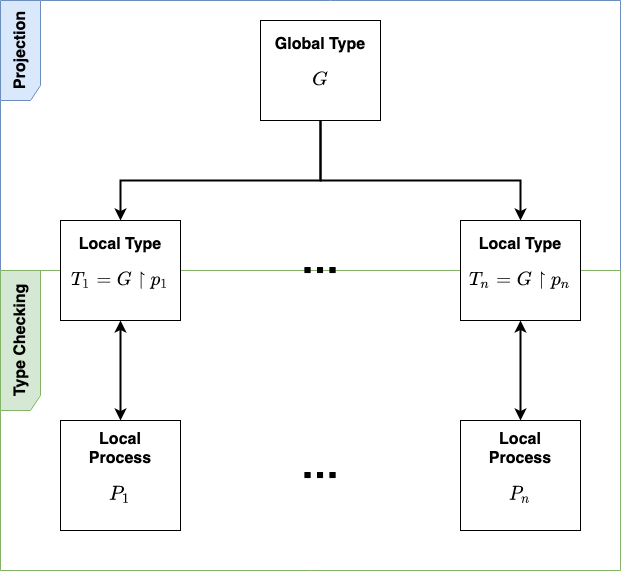
\includegraphics[width=.75\textwidth]{MpstFramework}
\caption{Type Checking with Multiparty Session Types}
\label{fig:mpstworkflow}
\end{figure}

\section{Related Work}
The two main approaches for incorporating our MPST workflow into application
development are native language support for first-class linear channel resources \cite{ATS} and code generation.
The latter closely relates to our proposal;
we highlight two areas of existing work under this approach that motivate our
design choice.

\paragraph{Endpoint API Generation}
Neykova and Yoshida targeted Python applications and the generation of runtime
monitors \cite{Python2017} to dynamically verify communication patterns.
Whilst the same approach could be applied to JavaScript, we can provide more
static guarantees with TypeScript's gradual typing system and compiler. Scribble-Java \cite{Hybrid2016} proposed to encode the EFSM
states and transitions as classes and instance methods respectively, with
behavioural typing achieved statically by the type system and channel linearity
guarantees achieved dynamically since channels are exposed and
aliasing is not monitored.
% REVIEW: could the approach of the present paper by applied to Java as well? discuss?
Scribble-Java can generate callback-style APIs similar to the approach we 
present, but this approach is arguably less idiomatic for Java developers.

\paragraph{Session Types in Web Development}
King et al. \cite{PureScript2019} targeted web development in PureScript using the
\textit{Concur UI} framework and proposed a type-level encoding of EFSMs as
multi-parameter type classes.
However, it presents a trade-off between achieving static linearity guarantees
from the type-level EFSM encoding under the expressive type system and
providing an intuitive development experience to developers, especially given
the prevalence of JavaScript and TypeScript applications in industry. Fowler \cite{MVU2019} focused on applying binary session types in front-end web
development and presented approaches that tackle the challenge of guaranteeing
linearity in the event-driven environment.

Our work applies the aforementioned approaches in a \textit{multiparty} context
using industrial tools and practices to ultimately encourage MPST-safe web
application development workflows in industry.

%\paragraph{Typestate programming} \dots



\section{TypeScript}
\label{section:typescript}

We introduce the TypeScript language 
\cite{UnderstandingTypeScript}
as our choice of target language
for session type API generation.
Developed by \textit{Microsoft Research},
TypeScript is an extension to
JavaScript to address
the deficiencies of the latter in
\textit{developing} and \textit{maintaining}
large-scale complex applications.
Syntactically,
TypeScript is a \textit{superset} of JavaScript,
so every JavaScript program is a
TypeScript program.
The TypeScript Compiler is used
to compile a TypeScript program into JavaScript
source code; since
JavaScript is a dynamically typed langauge,
the compilation process features full type erasure.

We introduce specific language
features used to implement our API generation
solution throughout the report as needed;
here, we highlight the key properties
of the type system implemented in the language.

\paragraph{Structural Typing}
In a structural type system, type equivalence
is determined by \textit{shape} rather than by name
(which is the case in a \textit{nominal} type system).

Consider the following TypeScript code:

\begin{lstlisting}[language=javascript]
class ThisSquare {
	constructor(public side: number) { }
};

class ThatSquare {
	constructor(public side: number) { }
};

declare function area(sq: ThisSquare): number;

area(new ThisSquare(2));	// ok
area(new ThatSquare(2));	// ok (*@\label{line:structural1}@*)
area({ side: 2 });			// ok (*@\label{line:structural2}@*)
\end{lstlisting}

The \texttt{area} function takes a \texttt{ThisSquare}
as parameter.
Under a structural type system,
\cref{line:structural1,line:structural2}
will type-check, because \texttt{ThatSquare} and the object
literal created from scratch matches the \textit{shape}
of \texttt{ThisSquare} -- all of them have a \texttt{side}
property typed \lstonelinejs{number}.

In languages (e.g. Java) that use a nominal type system, 
\cref{line:structural1}
will not type-check because \texttt{ThatSquare} is not named
\texttt{ThisSquare}.

\paragraph{Gradual Typing}
In a gradual type system, a program can have parts
that are statically typed and other parts are dynamically
typed \cite{GradualTyping}.
TypeScript distinguishes dynamically typed code using
the \lstonelinejs{any} type.

\begin{lstlisting}[language=javascript]
// Invoke remote API
fetch('https://jsonplaceholder.typicode.com/todos/1')
	// Convert to JavaScript Object Notation
	.then((response: Response) => response.json())
	.then((json: any) => {
		// Up to the developer to correctly deserialise;
		// incorrect implementations will cause
		// runtime type error.
	});
\end{lstlisting}

The rationale for this decision in \cite{UnderstandingTypeScript}
is that, JavaScript programs tend to interact with
data of unspecified types (such as fetching data
from API calls over the network); these parts
need to be dynamically typed in order to give developers
a smooth transition into TypeScript, and for TypeScript
to be usable in a distributed system setting. \\

\noindent
Based on the compatibility of TypeScript
with JavaScript, 
we believe that TypeScript API generation for session-typed
web development best achieves our objective
of providing
developers with a workflow
that provides communication safety guarantees in \textit{modern
web programming}
through multiparty session types.
We argue that the type system of TypeScript,
along with other language features we introduce
throughout the course of the report, is sufficient
for implementing session type theory in a manner that
complements idiomatic web development practices.


\part{Implementing Server-Centric Topologies over WebSockets}
\label{part:server}

\chapter{\fancyname{SessionTS}: Session Type API Generation for TypeScript}
\label{chap:codegen}

In this chapter, we present
\fancyname{SessionTS},
a toolchain for generating TypeScript APIs that developers can
use to write web applications that conform to their specified
communication protocol.
The toolchain is publicly available at \cite{repo}.

\fancyname{SessionTS} supports communication protocols that define 
\emph{server-centric} topologies, meaning that: 
\textbf{(1)} there is exactly one participant executed on the 
Node.js runtime; 
\textbf{(2)} all other participants run on the web browser; and
\textbf{(3)} all non-server participants only communicate with the server.
Examples of such protocols include the \tprotocol{Noughts and Crosses}
multiplayer game (\cref{section:evalgame}) and the \tprotocol{ATM} protocol.
We relax this assumption in \cref{part:general}.

\section{Development Workflow}

We motivate our development workflow from previous work 
\cite{PureScript2019} by extending the Scribble toolchain
and generating APIs that integrate the developer's 
application logic
into the execution of the communication automata.

We visualise the workflow in \cref{fig:devworkflow} 
and provide a brief overview:

\begin{enumerate}

\item The developer supplies the communication protocol written in
Scribble (\cref{subsection:scribble}), 
stating the role (hereafter \textit{endpoint})
to generate APIs for,
and the code generation \textit{target} 
(i.e. whether the role runs on the server or the web browser).

\item \fancyname{SessionTS} delegates to the 
Scribble toolchain for verifying the well-formedness of
the protocol and expects to receive a DOT graph representation of
the endpoint FSM (\cref{subsection:efsm}). 
\fancyname{SessionTS} parses the endpoint's 
interactions from the DOT graph and generates TypeScript APIs
for the developer (\cref{subsection:apigen}) 
tailored to the specified target.

\item The developer implements their web application using the
generated APIs. Implementations that pass the type-checking phase
of the TypeScript Compiler are guaranteed to be free from 
communication errors by session type theory.

\end{enumerate}

\begin{figure}[!ht]
\centering
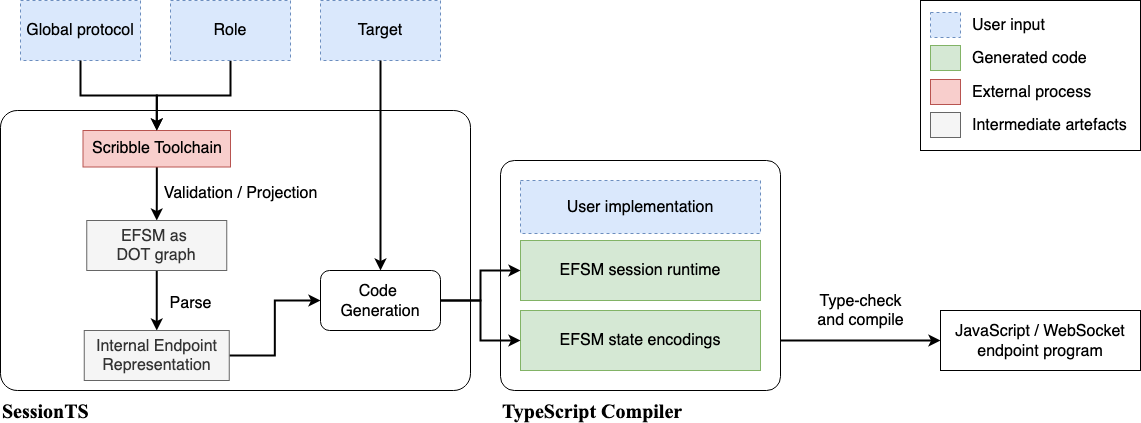
\includegraphics[width=\textwidth]{DevelopmentWorkflow}
\captionof{figure}{Overview of \fancyname{SessionTS} Development Workflow}
\label{fig:devworkflow}
\end{figure}

\subsection{Protocol Specification with Scribble}
\label{subsection:scribble}

We use the Scribble protocol description language, 
as presented in
\cite{Scribble}, for formalising the communication structure. This is
inspired by existing work on implementing session type theory 
in mainstream programming languages
\cite{Hybrid2016, PureScript2019, Python2017}. 
We use the variant of the Scribble language 
previously introduced in \cref{subsection:bgscribble}.

\subparagraph{Type declaration statements}
Specific to our TypeScript API generation toolchain,
the developer is \textit{not} required to explicitly
add type declaration statements for built-in types.
\cref{lst:adder} is a \textit{syntactically correct}
Scribble protocol as far as 
\fancyname{SessionTS} is concerned. 
Internally, \fancyname{SessionTS} inspects the protocol file
and parses existing type declarations using regular expressions
(or \textit{regex}) -- this is necessary to extract any
custom data types that will appear in the communication (for example,
\cref{lst:game}), and allows \fancyname{SessionTS} to inject
``boilerplate'' type declarations for built-in TypeScript types before
calling Scribble.

\begin{figure}[!ht]
\begin{lstlisting}[language=Scribble]
module Adder;

global protocol Adder(role Client, role Svr) {
	choice at Client {
		ADD(number, number) from Client to Svr;
		RES(number)         from Svr to Client;	
	} or {
		QUIT(string) from Client to Svr;	
		TERMINATE()  from Svr to Client;
	}
}
\end{lstlisting}
\captionof{lstlisting}{The \tprotocol{Adder} Protocol}
\label{lst:adder}
\end{figure}

We will use the \tprotocol{Adder} protocol as a running example
to demonstrate how our work performs TypeScript API generation.

\subsection{From Scribble to EFSM}
\label{subsection:efsm}

Given the protocol and endpoint, we use Scribble
to validate the well-formedness of the protocol and extract
information from the protocol relevant for the endpoint.
The latter is expressed as a finite state machine
where each state restricts the possible transitions, 
and transitions between states are represented by
communication actions, i.e. the sending or receiving of a message.

Scribble expresses the EFSM using the 
DOT graph description language \cite{dot}, with each
communication action encoded as the label of the corresponding
state transition. 
\fancyname{SessionTS} uses the pydot library \cite{pydot}
to parse the graph into an internal representation of the EFSM.
We define an \texttt{EfsmBuilder} class with APIs designed for
constructing the EFSM representation by iterating over the 
state transitions from the DOT representation.

\begin{figure}[!ht]
\begin{lstlisting}[language=Python]
@dataclass
class Endpoint:
    protocol: str
    role    : str
    server  : str
    efsm    : EFSM
    types   : typing.Iterable[DataType]
\end{lstlisting}
\captionof{lstlisting}{The Endpoint API}
\label{lst:endpointapi}
\end{figure}

As the code generation process requires additional information,
we define an \texttt{Endpoint} dataclass\footnote{
A Python dataclass uses the decorator to generate
``boilerplate'' methods, such as the constructor, based on the
properties listed in the annotations.} (\cref{lst:endpointapi})
to contain the \texttt{EFSM}
representation, along with the information passed in from the
command line (\texttt{protocol}, \texttt{role}, \texttt{server}) 
and the custom type declarations (\texttt{types}) parsed from the
protocol specification.

\subsection{API Generation}
\label{subsection:apigen}

Formally, API generation is a function of the constructed
\texttt{Endpoint} instance
\textit{and} the target specified in the command line. We use a 
different code generation strategy for implementations running on
the servre (\cref{chap:node}) versus the browser (\cref{chap:react}).
In this subsection, we explain how we perform API generation
at a higher level of abstraction.

Traditional methods of code generation involve applying the
Visitor pattern on the internal representation. 
In the context of the MPST framework,
this may involve defining a Visitor class that implements a
\texttt{generate()} operation to be performed on the EFSM states,
such that the \texttt{generate()} implementation specialises to the
type of EFSM state, i.e. send, receive or terminal.
This is not straightforward in Python, as method overloading is not 
supported, so the ``visit'' methods would need different names.
More importantly, it is less straightforward to visualise
the structure of the generated code, as the string interpolation
aspect is likely to be interleaved with source code implementing
additional logic for code generation.

For \fancyname{SessionTS}, we leverage the Jinja \cite{jinja} 
template engine library for code generation. 
We first construct templates for the TypeScript files we wish to generate,
specifying placeholders for dynamic content (to be extracted
from the \texttt{Endpoint} object); 
we then provide Jinja with the template path and the 
\texttt{Endpoint} object, and the template engine renders the
TypeScript code by filling in the dynamic placeholders. 
We show an example in \cref{lst:jinja}.

\begin{figure}[!ht]
\begin{lstlisting}[language=javascript, title=efsm.ts.j2]
export namespace Message {

  
  export type S{{ state ~ action.label }} = {
    label: Labels.S{{ state }}.{{ action.label }},
    payload: [{{ action.payloads|join(', ') }}],
  };
  
  export type S{{ state }} = 
  | S{{ state ~ action.label }};

\end{lstlisting}
\captionof{lstlisting}{Example Jinja Template for
\fancyname{SessionTS} API Generation}
\label{lst:jinja}
\end{figure}

Jinja provides lightweight syntax for injecting content and
markup for simple control structure: \texttt{\{\{ state \}\}} 
denotes a placeholder for Jinja to render the \texttt{state} variable,
and the \texttt{\{\% \%\}} syntax  is used for conditionals and
control structures 
(such as for loops, to dynamically render the enclosing ``sub-template''
by iterating over a collection).
The main advantage that Jinja brings is that 
it decouples the ``presentation''
from the ``content'' and makes it quick to prototype and extend
the generated code, \textit{usually} without modifications to the 
code generator.

\begin{figure}[!ht]
\begin{lstlisting}[language=python]
class CodeGenerationStrategy(ABC):

    target_to_strategy = {} (*@\label{line:mapping}@*)

    def __init__(self):
        super().__init__()

    @classmethod
    def __init_subclass__(cls, *, target):
        CodeGenerationStrategy.target_to_strategy[target] = cls (*@\label{line:register}@*)
        return super().__init_subclass__()
    
    @abstractmethod
    def generate(self, endpoint: Endpoint):
        pass
\end{lstlisting}
\captionof{lstlisting}{Implementing \texttt{CodeGenerationStrategy}}
\label{lst:codegenerationstrategy}
\end{figure}

As we generate a different set of TypeScript artefacts depending
on the specified target, we structure the different code generators
using the Strategy design pattern. Each target extends the
abstract base class \texttt{CodeGenerationStrategy} 
and implements its own \texttt{generate()}
method to return a list of \texttt{(path, content)} tuples. 
We define a \texttt{CodeGenerator} class that is parameterised 
by \texttt{target}: when instantiated, it will select and perform 
the specialised \texttt{generate()} method based on \texttt{target}, 
before formatting and committing the generated code 
to the file system.
We implement a subclass hook in \texttt{CodeGenerationStrategy}
(\cref{lst:codegenerationstrategy}),
such that each derived class must provide the target name to
``register'' with the base class (\cref{line:register}),
and the base class keeps an internal
mapping of the concrete strategies (\cref{line:mapping}); 
\texttt{CodeGenerator} accesses
this mapping to select the appropriate strategy.


\section{Implementation}

\codegen is written in Python. 
It offers flexible syntax, a rich standard library, and 
a healthy ecosystem of DOT graph parsers and template engines,
making it a suitable choice for implementing our code generator.
Its rich standard library also simplifies many tasks: we use
the \texttt{argparse} package to generate an informative
command line interface (CLI) for developers to 
supply the correct information (\cref{lst:cmdline})
to use \codegen
and the \texttt{subprocess} package to 
invoke external tools, such as Scribble and the TypeScript Compiler.

\begin{figure}[!ht]
\begin{lstlisting}
root@mpst_ts:/home# python3.7 -m mpst_ts --help
usage: __main__.py [-h] [-s SERVER] [-o OUTPUT]
                   filename protocol role {browser,node}

positional arguments:
  filename       Path to Scribble protocol
  protocol       Name of protocol
  role           Role to project
  {browser,node} Code generation target

optional arguments:
  -h, --help     show this help message and exit
  -s SERVER, --server SERVER
                 Server role (only applicable for browser targets)
  -o OUTPUT, --output OUTPUT
                 Output directory for generation
\end{lstlisting}
\captionof{lstlisting}{Entry Point for \codegen}
\label{lst:cmdline}
\end{figure}

We use Docker \cite{docker} to encapsulate our code generator
and its dependencies -- 
we found the canonical Python virtual environment
solution to be insufficient, as the Scribble toolchain is
a standalone Java executable with non-trivial setup procedures.
The Dockerfile builds a Docker image with Scribble and
the Python dependencies all pre-configured, and the provided
\texttt{build.sh} script instantiates the image as a container 
for development.
The \texttt{start.sh} script enters the Docker container
development environment and mounts the local project directory
onto the container as a volume to synchronise changes between the
two environments.

\section{Testing}
The challenge for testing \codegen
is to verify that the generated code is valid
TypeScript code.
Here, we detail our methodology
for \textit{system testing} -- 
executing \codegen end-to-end and testing
the generated code.

We implement a test suite on top of \texttt{unittest} APIs
for verifying that \codegen
generates \textit{valid TypeScript code}. This is especially useful as
our templates contain both TypeScript syntax and Jinja markup, 
so we cannot easily make sure that each template generates valid code,
let alone checking that the collection of templates generate a valid
TypeScript project altogether.

\begin{figure}[!ht]
\begin{lstlisting}[language=python,tabsize=4]
def test_code_generation(self):
	flags = [scr, protocol, role, target]
	if svr is not None:
		flags.append('-s')
		flags.append(svr)

	rc = mpst_ts.main(flags) (*@\label{line:testmain}@*)
	self.assertEqual(rc, 0)  (*@\label{line:testmainrc}@*)

	completion = subprocess.run(self.npm_test_cmd, shell=True) (*@\label{line:testtsc}@*)
	self.assertEqual(completion.returncode, 0) (*@\label{line:testtscrc}@*)

	shutil.rmtree(self.output_dir)
\end{lstlisting}
\captionof{lstlisting}{Main logic in \fancyname{SessionTS} system testing
test case}
\label{lst:systemtest}
\end{figure}

We provide a collection of Scribble protocols under \texttt{protocols/}
to generate test cases, one per protocol participant.
For each test case, the test suite (\cref{lst:systemtest}) will:

\begin{enumerate}
\item Invoke \fancyname{SessionTS} to generate the TypeScript project 
(\cref{line:testmain}), 
expecting a zero exit code (\cref{line:testmainrc});
\item Run the TypeScript Compiler on the generated directory 
(\cref{line:testtsc}),
passing the \texttt{noEmit} flag to purely perform type-checking,
and expecting a zero exit code (\cref{line:testtscrc}).
\end{enumerate}

As the generated TypeScript code makes assumptions about the
environment in which it is used (for example, having the \texttt{ws}
WebSocket package installed on server-side endpoints), we require a
\textit{sandbox environment} to type-check the generated code. 
The sandbox contains the minimal boilerplate required
for testing -- this involves having the WebSocket package installed
for server-side endpoints, the React.js framework (\cref{chap:react})
instantiated for browser-side endpoints,
and corresponding \texttt{tsconfig.json} files for both targets to
be picked up by the TypeScript Compiler.

For convenience, we extend the
Dockerfile and \texttt{build.sh} script 
to set up the sandbox environments. 
We also make use of the optional
\texttt{--output} flag exposed by the \fancyname{SessionTS} CLI
to redirect the generated code to the correct sandbox environment
to simply the testing process.

\chapter{\nodecodegen: Back-End Session Type Web Development}
\label{chap:node}

In this chapter we present \nodecodegen,
our session type API generation strategy for 
server-side endpoints implemented on the Node.js runtime 
\cite{nodejs}.
We continue to use the running example of the \tprotocol{Adder}
protocol (\cref{lst:adder}),
and refer to the FSM of the \trole{Svr} endpoint
(\cref{fig:addersvrfsm}) throughout this chapter.

We discuss the challenges of implementing
session types on the Node.js runtime 
(\cref{section:nodechallenges})
and motivate our approach (\cref{section:nodeapproach}).
We explain our design choices for encoding
the EFSM for server-side endpoints (\cref{section:nodeefsm}),
and present a session runtime designed
to execute the EFSM on Node.js (\cref{section:noderuntime}).
We conclude by analysing some alternative designs 
(\cref{section:nodealt}) and evaluating the limitations 
of our approach (\cref{section:nodelimitations}).

\begin{figure}[!b]
\centering
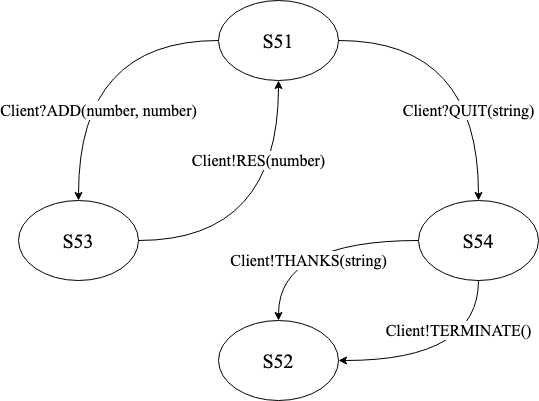
\includegraphics[width=0.6\textwidth]{AdderSvrFSM}
\captionof{figure}{\trole{Svr} Endpoint FSM
in \tprotocol{Adder} Protocol}
\label{fig:addersvrfsm}
\end{figure}

\section{Challenges}
\label{section:reactchallenges}

Our goal with \reactcodegen is to
generate session type implementations for the web browser.
Integrating session types into user interfaces is inherently difficult --
assuming channel actions are bound to user interface events 
(i.e. clicking a button sends a message), how does one formalise
channel linearity? How do we guarantee that, if the button
triggers a send at some EFSM state, that it triggers not more than
one channel action, \textit{and} the user cannot trigger the action
at another EFSM state?

We recap how existing work 
(as discussed in \cref{subsection:sessiontypewebdev})
tackle browser-side session typing.
Fowler \cite{MVU2020} introduced the concept of model types to 
prevent
channel linearity violation in his proposal for
integrating session types with
GUI programming, but
it uses the Links web programming language \cite{LINKS} which
lacks compatibility with the ecosystem of JavaScript
libraries that one might use in front-end development as well.
The session type-safe web development framework presented
by King et al. \cite{PureScript2019} generates APIs for
a functional target language in PureScript, and relies on
the \textit{Concur UI} framework that constructs UIs sequentially.

As motivated in \cref{section:intro},
we find these proposals to come at the cost of
limiting developer productivity by adopting unconventional practices
that may require a learning curve.
Through our work, we aim to distil the key
concepts from \cite{MVU2020,LINKS,PureScript2019} 
that provide session type safety
for web-based GUI programming, and implement them using
mainstream front-end web development tools (specifically TypeScript
and React), to provide developers with an intuitive way to implement
browser-side endpoints that guarantee communication safety.
\section{Approach}
\label{section:reactapproach}

We motivate our approach from \cite{MVU2020} by extending
their work on \textit{multiple model types} motivated by the
\textit{Model-View-Update} architecture (MVU),
introduced in \cref{section:bgrelated}.
The concept of model types express type dependencies between these
components: a \emph{model type} uniquely defines a \textit{view function},
set of \textit{messages} and \textit{update function} -- rather than
producing a new model, the update function defines valid transitions to
other model types.

We leverage the correspondence between model types 
and states in the EFSM:
each state in the EFSM is a model type, the set of messages represent
the possible channel actions available at that state,
and the update function defines which successor state to transition to,
given the supported channel actions at this state.

We implement model types for the EFSM on top of the 
\emph{React.js} (React) framework developed by Facebook \cite{React}.
React is widely used in industry to create scalable single-page
web applications, so this makes our workflow beneficial in an
industrial context. 
The framework defines a way for data to flow
between UI elements, and empowers the UI to subscribe and
``react'' to data changes;
we introduce the framework in \cref{subsection:react}.
We aim to implement similar behaviour with respect to the EFSM:
the UI should react to EFSM state transitions,
so we can \textbf{statically} ensure that the
channel actions ``present'' on the browser at any given time
are those permitted by the current EFSM state.

When executing \reactcodegen to generate code
for the \trole{Client} endpoint specifying the
\texttt{browser} target, the developer obtains the following 
groups of files:

\begin{itemize}

\item 
\textbf{S[40-43].tsx\footnote{
The \filename{.tsx} file extension allows
for embedding \textit{JSX} \cite{JSX} elements inside the file.
JSX is a XML-like syntax extension to JavaScript
for elements and components.
}:}
Developer APIs for implementing EFSM states 
(\cref{section:reactefsm});

\begin{itemize}
\item
\textbf{EFSM.ts}, \textbf{Message.ts}, \textbf{Roles.ts:}
Utility types for EFSM encoding;
\end{itemize}

\item 
\textbf{Client.tsx:} 
Session runtime for executing the EFSM 
(\cref{section:reactruntime});

\begin{itemize}
\item
\textbf{Session.ts}, \textbf{Types.ts:}
Utility types for session runtime.
\end{itemize}

\end{itemize}

\subsection{The React Framework}
\label{subsection:react}

We introduce the key features of the framework
through illustrating a web-based counter in \cref{lst:counter}.
The browser shows a counter (initialised to zero) 
and an ``Increment'' button:
when the user clicks on the ``Increment'' button,
the count is incremented and the UI shows the updated count.

\begin{figure}[!h]
\begin{lstlisting}[language=javascript,tabsize=2]
type Props = { count: number };
class Count extends React.Component<Props>{
	render() { (*@\label{line:childrender}@*)
		return <strong>{this.props.count}</strong>; (*@\label{line:childprops}@*)
	}
}

type State = { count: number };
class App extends React.Component<{}, State>{
	constructor(props: {}) {
		super(props);
		this.state = { count: 0 }; (*@\label{line:parentstate}@*)
	}
	
	increment() { this.setState({ count: this.state.count + 1 }); (*@\label{line:parentsetstate}@*)
	
	render() { (*@\label{line:parentrender}@*)
		return (<div>
			<button onClick={this.increment.bind(this)}>
				Increment
			</button>
			<Count count={this.state.count} /> (*@\label{line:childcomponent}@*)
		</div>);	
	}
}
\end{lstlisting}
\captionof{lstlisting}{Simple Counter in React}
\label{lst:counter}
\end{figure}

\paragraph{Components}
A \textit{component} is a reusable UI element which
contains its own mark-up and logic.
Components implement a \texttt{render()} method which returns
a React element, the smallest building blocks of a React application.
This is analogue to the \textit{view} function in the MVU architecture.
React uses the \textit{JSX} syntax extension \cite{JSX}
to interpolate TypeScript logic 
(enclosed in curly braces)
within HTML mark-up: 
in \cref{line:childrender}, the \texttt{Count} component
evaluates the TypeScript expression 
\lstonelinejs{this.props.count} and renders it in bold on the web page.

Components can render other components, which give rise to
a tree of UI elements. \cref{line:parentrender} shows that our
\texttt{Count} component is rendered by 
the \texttt{App} component.

\paragraph{Uni-directional Data Flow}
User-defined components derive from the abstract base class
\texttt{React.Component<P, S>},
which is an abstract base class with generic type parameters
\texttt{<P, S>} for \textit{props} (short for properties) and 
\textit{state} respectively.

The \texttt{App} component maintains \texttt{count} in its
state (\cref{line:parentstate}). Clicking on the increment button
updates the state (\cref{line:parentsetstate}), which invokes
a re-render, so the UI ``reacts'' to state change.

Data flows from parent components down to their children,
in the form of props. 
The \texttt{App} component passes the \texttt{count}
from its state to the \texttt{Count} component 
(\cref{line:childcomponent}), which accesses it via
\lstonelinejs{this.props}. 
Because \texttt{App} is re-rendered when the count is incremented,
the \texttt{Count} child component will also be re-rendered
with updated props.

\paragraph{Virtual DOM (VDOM) and Reconciliation}
The \texttt{render()} methods give the developer a declarative API
to specify what should be rendered. React uses a 
\textit{virtual DOM} abstraction, where the tree of React elements
are rendered on the virtual DOM, and React internally
runs a \textit{reconciliation} algorithm to update the browser DOM
accordingly using minimal operations.

For example, the \texttt{<button>} will not be re-rendered
on the browser DOM on every counter increment as it does not
depend on the updated state.

\section{EFSM Encoding}
\label{section:nodeefsm}

We show the structure of the generated EFSM.ts file in
\cref{lst:nodeefsmfile}.
Note that the formal definition of the EFSM in 
\cref{section:scribbleefsm}
contains more than just states and the state transition function,
so we encode the additional information as well.
Each type of information is grouped into their own
\textit{namespace}, and are collectively exported in
the EFSM \textit{module} for the developer to use.

\begin{figure}
\begin{lstlisting}[language=javascript,tabsize=2,title=EFSM.ts]
// (*@\cref{subsection:nodeefsmroleslabelsmsg}@*)
export namespace Roles {...};
export namespace Labels {...};
export namespace Message {...};

// (*@\cref{subsection:nodeefsmhandlers}@*)
export namespace Handler {...};

// (*@\cref{subsection:nodeefsmimplementation}@*)
abstract class ISend {...};
abstract class IReceive {...};
abstract class ITerminal {...};
export namespace Implementation {...};

export type EfsmTransitionHandler =
	(implementation: Implementation.Type) => void;
export type MessageHandler = (message: any) => void;
\end{lstlisting}
\captionof{lstlisting}{Structure of Generated EFSM Encoding 
for Server Endpoint}
\label{lst:nodeefsmfile}
\end{figure}

\subsection{Roles, Labels, Messages}
\label{subsection:nodeefsmroleslabelsmsg}

We generate TypeScript constructs for these pieces of information
so they can be reused throughout the generated code, 
and in particular, the runtime.

\subparagraph{Roles}
The runtime needs to know the identifiers of participants involved
in the session, and who to send/receive from 
depending on the EFSM state.
We generate string enumerations, or \textit{enums}, for each 
participant in the protocol, \textit{excluding} the 
first person endpoint. 
The enum appropriately groups the collection
of participants involved and scales for multiparty sessions,
whilst making it simple to derive other types, e.g. a mapping from
participants (indexed by the enum) to WebSockets.

\subparagraph{Labels}
The runtime needs to decide which handler to invoke, based
on the label of the received message. Similarly, the developer needs
to provide handlers specifying their internal choice (e.g. which
message label to send) and how to handle external choice (e.g. 
how to handle received message with particular label).
For the same reason, we also generate string enums for message labels,
one enum per state. Enums are compatible with switch statements,
which can be used to dispatch messages to the correct handlers
in the runtime based on the message label. 
We give an example in \cref{lst:nodeefsmlabels}.

\begin{figure}[!ht]
\begin{lstlisting}[language=javascript,tabsize=2]
// Inside the Labels namespace...
export enum S51 { ADD = "ADD", QUIT = "QUIT", };
export enum S53 { RES = "RES", };
export enum S54 { THANKS = "THANKS", TERMINATE = "TERMINATE", };
\end{lstlisting}
\captionof{lstlisting}{Generated Label Enums for \trole{Svr} endpoint}
\label{lst:nodeefsmlabels}
\end{figure}

\subparagraph{Messages}
The handler APIs that we generate for developers
need to refer to the label identifier and payload type: 
we refer to this as the message structure, and encode this as a
Message Type. 
Each message is expressed as an interface with
properties for the label and payload.
These interfaces are grouped based on the EFSM state
they belong using \textit{union types}.
We illustrate this in \cref{lst:addersvrmsg}.
By expressing the payload type as a \textit{tuple}\footnote{
In TypeScript, a tuple is an array with fixed size
and known types for elements at each position.
},
we easily generalise our type definition to polyadic payloads.

\begin{figure}[!ht]
\begin{lstlisting}[language=javascript, tabsize=2]
// Inside the Message namespace...
export interface S54THANKS {
	label: Labels.S54.THANKS,
	payload: [string],
};
export interface S54TERMINATE {
	label: Labels.S54.TERMINATE,
	payload: [],
};

export type S54 = | S54THANKS | S54TERMINATE;
\end{lstlisting}
\captionof{lstlisting}{Generated Message Type Definition for State 54}
\label{lst:addersvrmsg}
\end{figure}

\subsection{Handler APIs}
\label{subsection:nodeefsmhandlers}

We collect the APIs that the developer needs to implement
under the \texttt{Handler} namespace. 
As a design choice, we \textit{do not} generate handlers for
terminal states, because the semantics of inactivity mean
there is nothing to handle.
We introduce the generated handlers for sending and receiving states.
These are non-terminal states that will involve the encoding of its
successor state. The reader will notice that, in the listings below,
the successor state is stated to be under the
\texttt{Implementation} namespace: we explain in 
\cref{subsection:nodeefsmimplementation}, but for now,
it is sufficient to acknowledge that those refer to the encoding
of the successor state.

\subparagraph{Send}
We model selections using a union type to
encapsulate the possible send actions, as shown in 
\cref{lst:addersvrsendhandler}.
Each send action is encoded as a tuple of
the label, the payload, and the successor state encoding.
We see some benefits from defining Message Types as interfaces:
TypeScript supports \textit{index type queries} to extract
named property types, so
\lstonelinejs{Message.S54THANKS['payload']} 
would resolve to \lstonelinejs{[string]},
based on the interface definition \cref{lst:addersvrmsg}.

\begin{figure}[!ht]
\begin{lstlisting}[language=javascript, tabsize=2]
// Inside the Handler namespace...
export type S54 = 
	| [Labels.S54.THANKS, Message.S54THANKS['payload'],
			Implementation.S52] 
	| [Labels.S54.TERMINATE, Message.S54TERMINATE['payload'], 
			Implementation.S52];
\end{lstlisting}
\captionof{lstlisting}{Generated Type for \trole{Svr} Send State
in \tprotocol{Adder} protocol}
\label{lst:addersvrsendhandler}
\end{figure}

We generalise deterministic send actions as a trivial \textit{selection}, 
as motivated from the theory (\cref{fig:globaltypes}),
so the encoding for State 53 in the \trole{Svr} FSM would be
the union of a single tuple.

\subparagraph{Receive}
We model branching using an interface to 
enumerate the possible branches, as shown in
\cref{lst:addersvrreceivehandler}.
As with send states,
we generalise deterministic receive actions as a trivial \textit{branch},
which would be an interface with one property. 

\begin{figure}[!ht]
\begin{lstlisting}[language=javascript,tabsize=2]
// Inside the Handler namespace...
export type S51 = {
	[Labels.S51.ADD]: (...payload: Message.S51ADD['payload']) =>
		Implementation.S53,
	[Labels.S51.QUIT]: (...payload: Message.S51QUIT['payload']) => 
		Implementation.S54,
}
\end{lstlisting}
\captionof{lstlisting}{Generated Type for \trole{Svr} Receive State
in \tprotocol{Adder} protocol}
\label{lst:addersvrreceivehandler}
\end{figure}

The interface properties are defined by the 
labels of the permitted receive actions:
the square-bracket notation means that the property name
is derived from the value of the enclosing variable,
so \lstonelinejs{[Labels.S51.ADD]} resolves to the
\lstonelinejs{'ADD'} string. 

The interface values are functions parameterised by
the message payload, and must return the successor state encoding.
We see another benefit of defining the payload in Message Types
as a tuple: we can define the receive handler parameter
using the \textit{spread syntax}, which allows the tuple
expression to be expanded into a list of function arguments. 
More concretely, as shown in \cref{lst:nodeefsmspread},
it allows the developer to pattern match on the
individual payload values (\cref{line:yesspread}) 
rather than defining their function to expect a tuple 
and manually destructing it (\cref{line:nospread}),
so the former is more intuitive.

\begin{figure}[!ht]
\begin{lstlisting}[language=javascript,tabsize=2]
const withSpread = (x: number, y: number) => {...} (*@\label{line:yesspread}@*)
const withoutSpread = (payload: [number, number]) => {...} (*@\label{line:nospread}@*)

const handler1: Handler.S51 = { ADD: withSpread		, ... };	// OK
const handler2: Handler.S51 = { ADD: withoutSpread, ... };	// OK
\end{lstlisting}
\captionof{lstlisting}{Example Handler Signature 
Compatible with Spread Syntax}
\label{lst:nodeefsmspread}
\end{figure}

\subsection{Wrapping Handlers in ``Implementations''}
\label{subsection:nodeefsmimplementation}

The behaviour of the runtime is dependent on the current state,
so it needs a way to distinguish between
all the different states -- one can think of this as implementing
the state transition function from the theory, which is analogue to 
overloading a \texttt{next()} method for each state.
Due to limitations in the TypeScript language, this would have to
be some sort of switch statement, with the \texttt{next()}
method parameterised by some base type assignable to all states.
Currently, the state is only determined by the handler
to be implemented by the developer, so the switch statement
and base type would have to be defined on the handler APIs.

Unfortunately, this is not practical. 
Handlers for send states are union types and
handlers for receive states are interfaces,
both of which are not supported 
by the \lstonelinejs{instanceof}
operator.

\subsubsection{Distinguishing Handlers using Conditional Types}

We attempt to address this by defining an enum of state identifiers
for each type of state (i.e. an enum for send states, 
an enum for receive states)
upon which to execute the EFSM, which solves the switch statement
problem.
Now, we are left with defining a mapping between the 
state identifier enum to the handler type. This construct would be
analogue to \textit{dependent types}, which again, is not a feature
of the TypeScript type system.

We try to define type dependencies using
\textit{conditional types} in TypeScript.
A conditional types is a type-level expression
\begin{lstlisting}[language=javascript,numbers=none]
T extends U ? X : Y;
\end{lstlisting}
which reads, \textit{if \texttt{T} is assignable to \texttt{U},
then the type is \texttt{X}; otherwise, the type is \texttt{Y}}.

Combined with \textit{generic constraints}\footnote{
\lstonelinejs{<T extends U>} defines a generic type \texttt{T}
and enforces that it must be a type assignable to \texttt{U}.
},
we can approximate the dependency between the state identifier
enum and the generated handler API using something
similar to \cref{lst:conditionaltypes}.

\begin{figure}[!h]
\begin{lstlisting}[language=javascript,tabsize=2]
enum SendState { S1, S3, ... };
enum ReceiveState { S2, S4, ... };
type State = SendState | ReceiveState;

type SendHandler<S extends SendState> = 
	S extends SendState.S1 ? Handler.S1 :
	S extends SendState.S3 ? Handler.S3 : ... ;

type ReceiveHandler<S extends ReceiveState> = 
	S extends ReceiveState.S2 ? Handler.S2 :
	S extends ReceiveState.S4 ? Handler.S4 : ... ;
\end{lstlisting}
\captionof{lstlisting}{Approximating Type Dependency
using \textit{Conditional Types}}
\label{lst:conditionaltypes}
\end{figure}

We intend to use this construct when defining the EFSM transition
function for the runtime, for each type of state,
so the method signature for transitioning to send states
would resemble \cref{lst:conditionaltransitionfunction}

\begin{figure}[!h]
\begin{lstlisting}[language=javascript,numbers=none]
declare function transitionToSend<S extends SendState>(
	stateId: S, handler: SendHandler<S>
);
\end{lstlisting}
\captionof{lstlisting}{EFSM Transition Function 
using Conditional Types}
\label{lst:conditionaltransitionfunction}
\end{figure}

Unfortunately, this approach does not work for the simple fact that
conditional types were not designed to be exploited in this manner.
The main limitation of conditional types is its 
\textit{distributivity} when the type ``parameter'' is an
union type (which is the case for enums, as
\texttt{S = SendState.S1 | SendState.S3 | ...}), where

\begin{lstlisting}[language=javascript,numbers=none]
(T1 | T2) extends U ? X : Y
\end{lstlisting}

results in the conditional type being \textit{distributed}
among each constituent,

\begin{lstlisting}[language=javascript,numbers=none]
(T1 extends U ? X : Y) | (T2 extends U ? X : Y)
\end{lstlisting}

so the type expression returns to an union type,

\begin{lstlisting}[language=javascript,numbers=none]
X | Y
\end{lstlisting}

Returning to \cref{lst:conditionaltransitionfunction}, 
the type of \texttt{handler} will end up being a union type, 
rather than the ``dependent type''
construct we were hoping for.

\subsubsection{Distinguishing Handlers using Discriminated Unions}

Instead, we leverage \textit{discriminated unions}: all members
of the union type share a common property (the \textit{discriminant})
of which they each define an
unique value for, so that the TypeScript Compiler can refine the union
to the specific constituent upon checking the value of the discriminant
(e.g. applying a switch statement).

For the time being,
it is sufficient to understand that for each EFSM state,
in addition to the API defined under the
\texttt{Handler} namespace, it also has a wrapper API defined under
the \texttt{Implementation} namespace (\cref{lst:nodeefsmimplementation}),
which defines the \texttt{type}
discriminant property internally. This explains why the successor
state encodings in 
\cref{lst:addersvrsendhandler,lst:addersvrreceivehandler}
were defined as such.

\begin{figure}[!h]
\begin{lstlisting}[language=javascript,tabsize=2]
abstract class ISend { type: 'Send' = 'Send'; ... }
abstract class IReceive { type: 'Receive' = 'Receive'; ... }

export namespace Implementation {

	export class S51 extends IReceive {
		constructor(private handler: Handler.S51) { super(); }
		...
	}
	...
};
\end{lstlisting}
\captionof{lstlisting}{Discriminated Unions in EFSM 
for Server-Side Endpoints}
\label{lst:nodeefsmimplementation}
\end{figure}

We discuss our runtime implementation shortly 
(\cref{section:noderuntime}), where we disclose more details regarding
the role of the \texttt{Implemenation} wrapper API in
the runtime.
\section{Runtime}
\label{section:noderuntime}

We define the session runtime for the \trole{Svr} endpoint
of the \tprotocol{Adder} protocol in \filename{Svr.t}s,
named after the endpoint.
It exposes a \textbf{public API}
with seams for the developer to pass in the WebSocket server 
and application logic
(i.e. implementations of the handler APIs).
It is developer's responsibility to construct the
WebSocket server and set it up to listen for incoming connections.
Internally, it keeps a \textit{private API}
for executing the EFSM, when all participants have 
joined the session.

\begin{lstlisting}[language=javascript]
// Exported to developer
export class Svr {
	constructor(wss: WebSocket.Server,
				initialState: Implementation.S51) { ... }
	...
}

// Not exported to developer
class Session {
	private wss: WebSocket.Server;
	private initialState: Implementation.S51;
	private roleToSocket: RoleToSocket;
	...
}
\end{lstlisting}

The role of the public API is to manage incoming connections and
wait for all participants to join the session 
(\cref{subsection:noderuntimepublic}), before
handing off to the private API to execute the EFSM
(\cref{subsection:noderuntimeprivate}).

\subsection{Managing Connections}
\label{subsection:noderuntimepublic}

The constructor of the public API class sets up
the framework for mapping incoming WebSocket connections to
participants. 
The main challenge is to wait for all participants to 
connect to the server endpoint before EFSM execution begins.
We address this by defining an internal protocol for managing
session joining -- since we generate the runtime for both server 
and browser endpoints, we can implement this in a way that is 
transparent to the developer.

\begin{figure}[!h]
\begin{lstlisting}[language=javascript,tabsize=2]
const waiting: Set<Roles.Peers> = new Set([Roles.Peers.Client]); (*@\label{line:initwaiting}@*)

// Mapping of roles to WebSocket connections
const roleToSocket: Partial<RoleToSocket> = { (*@\label{line:initroletosocket}@*)
	[Roles.Peers.Client]: undefined,
};

// Invoked when a connection request is received
const onSubscribe = ({ data, target: socket }) => {

	// Deserialise connection request message
	const { connect: role } = JSON.parse(data) 
		as Message.ConnectRequest; (*@\label{line:connectionrequest}@*)
		
	// Ignore if role is already taken
	if (!waiting.has(role)) { return socket.close(); } (*@\label{line:occupied}@*)
	
	// Map the role in the connection request to this WebSocket
	roleToSocket[role] = socket; (*@\label{line:connectwsbind}@*)
	waiting.delete(role);
	
	// Start executing EFSM when all roles have joined
	if (waiting.size === 0) {
		new Session(wss, roleToSocket as RoleToSocket, initialState); (*@\label{line:newsession}@*)
	}
};

// For every new connection, process message with `onSubscribe`
wss.addEventListener('connection', ws => {
	ws.onmessage = onSubscribe; (*@\label{line:wslisteneroverride}@*)
});
\end{lstlisting}
\captionof{lstlisting}{Handling Connections in Server Endpoint}
\label{lst:nodeconnect}
\end{figure}

We show this in \cref{lst:nodeconnect} and walk through
the main parts:

\begin{enumerate}
\item
The server keeps track of the participants that 
have yet to join the session -- this is initialised to the
complete set of
non-server endpoints at the start (\cref{line:initwaiting}).

\item
Browser endpoints request to join the session
by sending a \textit{connection request} with the role
identifier as payload (\cref{line:connectionrequest}). 
We generate role enums for browser targets
in the same way, so the server can correctly
interpret the message.
We listen to connection requests by overriding the
\texttt{onmessage} event listener for every new connection
(\cref{line:wslisteneroverride}).

\item
If the role is already occupied, then the server
responds by closing the connection (\cref{line:occupied}).

\item
Otherwise, the role is not occupied, so the server binds
the WebSocket (which the message was received from) to the role
(\cref{line:connectwsbind}).
This is accumulated in an interface type, mapping each
role to an \textit{optional}\footnote{
TypeScript provides utility types for common type transformations:
\texttt{Partial<T>} constructs a type with all properties
of \texttt{T} set to optional.
} 
WebSocket property
-- for roles who have
not yet connected, we do not know the WebSocket binding, so the
WebSocket for these roles are \lstonelinejs{undefined},
as initialised at the start (\cref{line:initroletosocket}).

\item
When the server is no longer waiting for any participants,
it notifies all other roles through the bounded WebSocket
connections that the session will start, and delegates
EFSM execution to the private API by constructing
an instance of the \texttt{Session} class (\cref{line:newsession}).
The notification process is managed by the \texttt{Session} class.

\begin{lstlisting}[language=javascript,tabsize=2,numbers=none]
Object.values(roleToSocket).forEach(socket => {
	socket.send(JSON.stringify(Message.ConnectConfirm));
});
\end{lstlisting}

\item
We define the interfaces and factories for connection messages 
in the generated EFSM.ts file under
the \texttt{Message} namespace.

\begin{lstlisting}[language=javascript,tabsize=2,numbers=none]
// Inside the Message namespace...
export interface ConnectRequest { connect: Role.Peers };
export const ConnectConfirm = { connected: true };
\end{lstlisting}
\end{enumerate}

\subsection{Executing the EFSM}
\label{subsection:noderuntimeprivate}

The \texttt{Session} class executes the EFSM.
We define a transition function, \texttt{next()}, 
parameterised by the current state,
The constructor of the \texttt{Session} class
explicitly calls \texttt{next()} with the 
initial state implementation provided by the developer
to start EFSM execution.
\texttt{next()} invokes the handler defined by the developer
and performs the required channel actions for non-terminal states.

\begin{itemize}
\item 
For \textbf{send} states, the handler will
return the label and payload to be sent, along with the
successor state implementation. The transition function
should construct and send the message, 
and transition to the successor state.

\item
For \textbf{receive} states, we change the
message event listener on the WebSocket to
pass the incoming message to the handler.
The handler will return the successor state,
which the runtime can transition to.

\end{itemize}

We conceptualise this in \cref{lst:noderuntimesimple}.
The discriminated union lets the runtime figure out
the type of the current state.

\begin{figure}[!h]
\begin{lstlisting}[language=javascript,tabsize=2]
next(state: Implementation.Type) {
	// Distinguish between states using discriminant property
	switch (state.type) {
		case 'Send': {
			const [label, payload, succ]: (*@\hl{???}@*) = state.handler;	 (*@\label{line:noderuntimebadtype1}@*)
			this.send((*@\hl{???}@*), label, payload);	// Who to send to? (*@\label{line:noderuntimeunknownrole}@*)		
			return this.next(succ);
		}
		case 'Receive': {
			// Handle incoming messages using this anonymous function
			this.wss.onmessage = ({ data }) => {
			
				// Which message structure to use to deserialise?
				const { label, payload } = JSON.parse(data) as (*@\hl{???}@*); (*@\label{line:noderuntimebadtype2}@*)
				const succ: (*@\hl{???}@*) = state.handler[label](...payload); (*@\label{line:noderuntimebadtype3}@*)
				return this.next(succ);
			}
		}
		case 'Terminate': { return; }
	}
}
\end{lstlisting}
\captionof{lstlisting}{Conceptual EFSM Transition Function 
for Server-Side Endpoint}
\label{lst:noderuntimesimple}
\end{figure}

However, we still face problems with resolving types, as highlighted.
Just because we know that the current state is a send state,
we do not know \textit{which} particular state it is,
so we cannot accurately type the handler (\cref{line:noderuntimebadtype1}).
The same problem is amplified for the receive state:
we need to know the specific receive state in order
to correctly serialise the message (\cref{line:noderuntimebadtype2})
and interpret the successor state (\cref{line:noderuntimebadtype3}).
We see another problem with handling send states:
because we do not know the specific send state, we do not know which
participant to send the message to (\cref{line:noderuntimeunknownrole}).

\begin{figure}[!h]
\begin{lstlisting}[language=javascript,tabsize=2]
abstract class ISend {
	type: 'Send' = 'Send';
	abstract performSend(
		next: EfsmTransitionHandler,
		send: (role: Roles.Peers, label: string, payload: any[]) 
			=> void,
	): void;
};

abstract class IReceive {
	type: 'Receive' = 'Receive';
	abstract prepareReceive(
		next: EfsmTransitionHandler,
		register: (from: Roles.Peers, messageHandler: MessageHandler)
			=> void,
	): void;
};
\end{lstlisting}
\captionof{lstlisting}{Class Definitions for \texttt{Implementation} API}
\label{lst:nodeabstractclass}
\end{figure}

These all reduce to the same core problem: the runtime
needs to know the specific state at compile-time\footnote{
Whether TypeScript ``compiles'' or ``transpiles''
(or even \textit{``transcompiles''} \cite{transcompiles}) to JavaScript
is not relevant to our work; we stick with compilation
and keep our terminology consistent.}.
We solve this through \textit{runtime polymorphism} instead, since
the specific type of \texttt{state} is known at runtime.
For each type of state, we define a common API that can be invoked
by the EFSM transition function. To achieve runtime polymorphism,
each concrete state must provide a specific implementation: 
this motivates our design for defining the discriminated union
using abstract classes with abstract methods 
(\cref{lst:nodeabstractclass}).

\begin{figure}[!h]
\begin{lstlisting}[language=javascript,tabsize=2]
next(state: Implementation.Type) {
	switch (state.type) {
		case 'Send':				// recall (*@\cref{lst:nodeefsmimplementation} \cref{line:nodeefsmsend}@*)
			return state.performSend(this.next, this.send);
		case 'Receive':			// recall (*@\cref{lst:nodeefsmimplementation} \cref{line:nodeefsmreceive}@*)
			return state.prepareReceive(this.next, this.register);
		case 'Terminal':		// recall (*@\cref{lst:nodeefsmimplementation} \cref{line:nodeefsmterminal}@*)
			return;
	}
}
\end{lstlisting}
\captionof{lstlisting}{Final EFSM Transition Function for Server-Side
Endpoint}
\label{lst:noderuntime}
\end{figure}

Using this approach,
we can pass the transition function and channel actions 
from the \texttt{Session} runtime class
to the individual state \texttt{Implementation} classes:
these are also generated by \fancyname{NodeTS}, so we
guarantee linear usage of channel resources by construction as well.
This \textit{significantly} simplifies the design of the runtime
(\cref{lst:noderuntime}),
because the transition function no longer needs to know the type 
of the specific state at compile-time.

By passing the specific functions defined in the runtime
to the individual EFSM states, we can visualise our runtime
as a \textit{message passing} abstraction 
(\cref{fig:noderuntimeefsm}): the runtime uses the common
\texttt{performSend()} or \texttt{prepareReceive()} API
to delegate to the specialised implementation, which will in turn
ask the runtime to perform specialised channel actions using
the parameterised methods, and finally delegate back to
the runtime to transition to the specific successor state.

\begin{remark}
We need to be careful when passing \textit{instance} methods
as \textit{function} arguments 
-- namely, the semantics of \lstonelinejs{this} is different.
In short, we have to \textit{explicitly}
\texttt{bind()} the \texttt{Session} object
to the instance methods that we pass as function arguments:

\begin{lstlisting}[language=javascript,tabsize=2]
// Inside the Session class constructor...
this.next = this.next.bind(this);
this.send = this.send.bind(this);
this.register = this.register.bind(this);
\end{lstlisting}

Not doing so will result in \lstonelinejs{this} taking
a different value 
(either the global object or \lstonelinejs{undefined}).
\end{remark}

We elaborate on how this mechanism
handles the sending and receiving of messages in
\cref{subsection:noderuntimesend,subsection:noderuntimereceive}
respectively.

\begin{figure}[!ht]
\centering
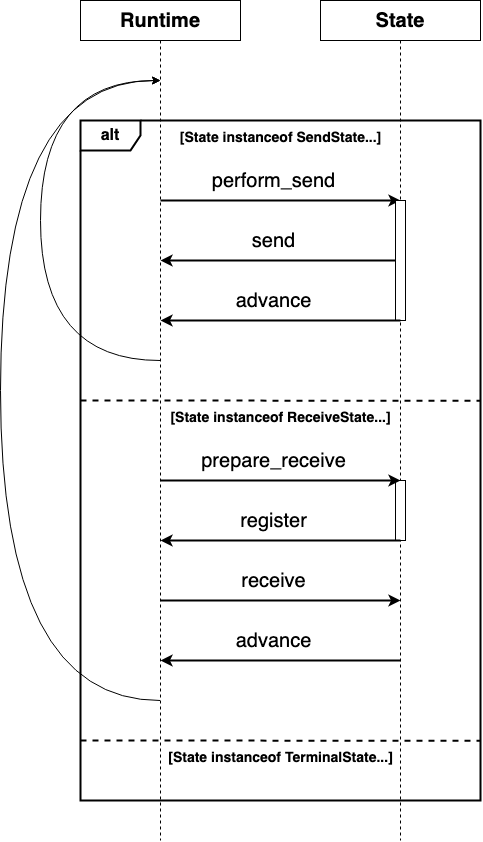
\includegraphics[width=0.5\textwidth]{NodeRuntimeEFSM}
\captionof{figure}{``Message Passing'' Abstraction of EFSM Execution for
Server Endpoints}
\label{fig:noderuntimeefsm}
\end{figure}

\subsection{Sending Messages}
\label{subsection:noderuntimesend}

This is rather straightforward: 
we show the generated code in \cref{lst:nodesend}.

\begin{figure}[!h]
\begin{lstlisting}[language=javascript,tabsize=2]
export class S54 extends ISend {
	constructor(private handler: Handler.S54) { super(); }

	performSend(
		next: EfsmTransitionHandler,
		send: (role: Roles.Peers, label: string, payload: any[]) 
			=> void
	) {
		const [label, payload, successor] = this.handler;
		send(Roles.Peers.Client, label, payload); (*@\label{line:nodesendrole}@*)
		return next(successor);
	}
}
\end{lstlisting}
\captionof{lstlisting}{Generated Code for \texttt{Implementation} API for
Send State}
\label{lst:nodesend}
\end{figure}

We get the label, payload and successor implementation
directly from the handler implemented by the developer, 
accurately typed by how we define the handler API in \filename{EFSM.ts}.
The developer does not need to specify which role
to send to: this is a sensible design choice, as we know this
from the Scribble protocol, so we do not need the developer 
to specify separately.
As a result, we generate the code to send the message
to the correct role (\cref{line:nodesendrole}).
We use the \texttt{send()} method passed down
by the runtime to commit our communication action:
the runtime will handle how to serialise the message and perform
the send. We guarantee that \texttt{send()} is called
\textbf{exactly once} by construction, thus channel linearity
is never violated.
Finally, we use the parameterised EFSM transition handler
to notify the runtime which specific state to transition to.

\subparagraph{Sending through WebSockets}
We define message structures as interfaces, which
are represented by objects. 
By convention in \fancyname{SessionTS},
we serialise messages into \textit{JavaScript Object Notation}
(or JSON) \cite{json} using the built-in \texttt{JSON.stringify()}
method.

\begin{lstlisting}[language=javascript]
send(role: Roles.Peers, label: string, payload: any[]) {
	this.roleToSocket[role].send(JSON.stringify({
		label, payload
	});
}
\end{lstlisting}

They are decoded using the same interface schema on the receiving end
using \texttt{JSON.parse()}.
Whilst the method return type is the
dynamic \lstonelinejs{any} type, 
we guarantee type safety by construction
as we performed the serialisation in the first place, so
we can safely interpret the deserialised content 
using a concrete type.

\subsection{Receiving Messages}
\label{subsection:noderuntimereceive}

We need to update the message event listener on the WebSocket
to use the developer's handler -- 
specific to the \textit{current state} -- 
to process the message.
Our approach is to keep the WebSocket message event listener
untouched, but define it in a way that allows \textit{dynamic} behaviour.
We walk through the concept implemented in (\cref{lst:noderuntimewsmsg}):

\begin{enumerate}
\item 
\texttt{Session} keeps track of the \textit{current}
message receive handler (\cref{line:noderuntimehandler}).
The \texttt{?} syntax denotes it is an \textit{optional}
type: not every state is a receive state, so there does not \textit{have} to
be an active message handler.

\item
The receive handler does \textit{not} need a specialised type
(\cref{line:msghandler}). The receive handler is defined in
the \texttt{Implementation} class of the concrete receive state,
so it will deserialise the message to the correct form.

\item
The \texttt{register()} method (\cref{line:register})
is passed to the \texttt{Implementation} class of the concrete
receive state, which will construct the message handler
around the developer's handler implementation and register it
with the runtime.

\item
When a message is received from the channel,
we dynamically process it with 
the current registered handler (\cref{line:callhandler}).
We encapsulate this dynamic behaviour in an instance method
and bind it as an event listener (\cref{line:wsbind})
for the WebSocket connection
of each non-server endpoint.
\end{enumerate}

\begin{figure}[!h]
\begin{lstlisting}[language=javascript,tabsize=2]
type MessageHandler = (message: any) => void; (*@\label{line:msghandler}@*)

class Session {
	// Optional type, same as `MessageHandler | undefined`
	private handler?: MessageHandler; (*@\label{line:noderuntimehandler}@*)

	constructor(...) {
		...
		// Process incoming messages from each WebSocket
		// using `this.receive()`
		Object.values(this.roleToSocket).
			.forEach(ws => ws.onmessage = this.receive.bind(this)); (*@\label{line:wsbind}@*)
			
		// Initialise handler as undefined
		this.handler = undefined;
	}
	
	// Set the handler to be used to handle the next receive event
	register(handler: MessageHandler) { this.handler = handler; } (*@\label{line:register}@*)

	receive({ data }: WebSocketMessage) {
		const handler = this.handler; (*@\label{line:callhandlerstart}@*)
		
		// `Unregister` the current receive handler
		this.handler = undefined; (*@\label{line:callhandler2}@*)
		
		// `handler` has an optional type, so we first
		// check if there is a value set, then invoke the handler.
		// Same as `if (handler !== undefined) { handler(data); }`
		handler?.(data); (*@\label{line:callhandler}@*)
	}
}
\end{lstlisting}
\captionof{lstlisting}{Attempt to Dynamic WebSocket Message Event Listener}
\label{lst:noderuntimewsmsg}
\end{figure}

We also show the generated code for the \texttt{Implementation}
class of the receive state in \cref{lst:nodereceive}
-- this should appear consistent
with the explanation above.

\begin{figure}[!h]
\begin{lstlisting}[language=javascript,tabsize=2]
export class S51 extends IReceive {
	
	constructor(private handler: Handler.S51) { super(); }

	prepareReceive(
		next: EfsmTransitionHandler,
		register: (from: Roles.Peers, messageHandler: MessageHandler)
			=> void
	) {
		// Define dynamic WebSocket message event listener
		const messageHandler = (message: any) => {
		
			// Deserialise message
			const decoded = JSON.parse(message) as Message.S51;
			
			// Discriminate between messages using label
			switch (decoded.label) {
				case Labels.S51.ADD: {
					// Invoke handler to get successor state
					const successor = 
						this.handler[decoded.label](...decoded.payload);
						
					// Invoke callback to advance EFSM
					return next(successor);
				}
				case Labels.S51.QUIT: {
					const successor = 
						this.handler[decoded.label](...decoded.payload);
					return next(successor);	
				}
			}            
		}
		
		// Register the message handler under the
		// WebSocket bound to the `Client` role
		register(Roles.Peers.Client, messageHandler);
	}
}
\end{lstlisting}
\captionof{lstlisting}{Generated Code for \texttt{Implementation} API for
Receive State}
\label{lst:nodereceive}
\end{figure}

Ideally, a more succinct (and direct) representation would be
\begin{lstlisting}[language=javascript]
(message: any) => {
	const decoded = JSON.parse(message) as Message.S51;
	const successor = 
		this.handler[decoded.label](...decoded.payload);
	return next(successor);
}
\end{lstlisting}

But this expresses a type dependency between \texttt{label}
and \texttt{payload} which, as discussed 
(\cref{subsubsection:dependenttypes}), cannot be implemented.
However message structures \textit{precisely} 
define a discriminated union 
(the label acts as the discriminant 
to distinguish between payload types),
so we handle this with a switch statement,
at the cost of having the same code in each case --
TypeScript does infer the correct specific type in each case statement,
so code duplication here does serve a functional purpose.

Returning to \cref{lst:noderuntimewsmsg},
note that the type of the \texttt{handler} property is \textit{optional}
-- this hints at a problem: 
\textit{how do we know that \texttt{this.handler} is set when
a message is received?} The types imply that we \textit{do not},
and this is indeed the case.
In fact, when we consider a \textit{multiparty} context,
our approach with receive handler registration 
using an optional value actually \textit{fails} to guarantee correctness.
We motivate the problem with a worked
example.

\begin{example}[``Out-of-order'' message receives]
Recall that Node.js is a single-threaded event loop runtime, so
when a message arrives, 
the \texttt{onmessage} event is \textit{queued},
and current execution is \textit{not pre-empted}.

Now consider a multiparty session specified by the global type

\[
A \to S: \text{\lstonelinejs{M1(string)}}.~ 
B \to S: \text{\lstonelinejs{M2(number)}}.~\texttt{end} 
\]

Suppose \trole{S} is the server endpoint.
We describe a possible execution flow for the protocol
that breaks our implementation:

\begin{enumerate}
\item 
\trole{S} transitions to its initial state, 
``receive \lstonelinejs{M1(string)} from \trole{A}''.
The receive handler for \tmsg{M1} is registered.

\item
\tmsg{M2} arrives at \trole{S}, so the \texttt{onmessage} handler
is queued. This is \textit{perfectly plausible}: there
is no causal relation between \tmsg{M1} and \tmsg{M2}.

\item
\tmsg{M1} arrives at \trole{S}, so the \texttt{onmessage} handler
is queued.

\item
The \texttt{onmessage} handler for \tmsg{M2} is executed.
The registered handler expects \lstonelinejs{M1(string)},
but it is called with \lstonelinejs{M2(number)}, which raises
a runtime type error.
\end{enumerate}

This exposes a problem: 
the order of message \textit{arrivals} may not
correspond with the order of \textit{receiving} messages as
specified in the protocol,
\textit{so} the message may arrive before its
corresponding handler is registered.
\end{example}

We observe that message arrivals do not have to be causally related.
However, if we consider a similar \textit{binary} example
\[
A \to S: \text{\lstonelinejs{M1(string)}}.~ 
A \to S: \text{\lstonelinejs{M2(number)}}.~\texttt{end}
\]
then \tmsg{M1} \textit{must} arrive before \textit{M2},
since this is sent through the WebSocket connection between 
\trole{A} and \trole{S}, and FIFO guarantees are respected 
for each individual WebSocket connection. 
We visualise the possible orders of message receive events
in \cref{fig:nodereceivecompare}.

\begin{figure}[!h]
\centering
\begin{subfigure}[b]{0.8\textwidth}
\centering
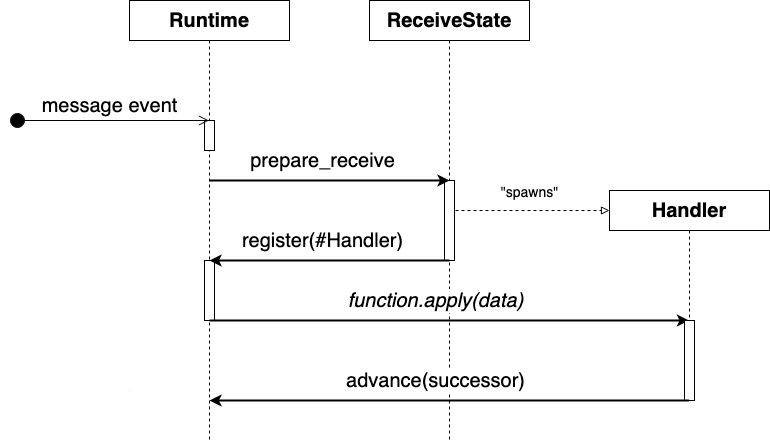
\includegraphics[width=\textwidth]{NodeRuntimeReceive2}
\caption{Message processed before transitioning to receive state}
\label{subfig:nodereceivemsgfirst}
\end{subfigure}
\hfill
\begin{subfigure}[b]{0.8\textwidth}
\centering
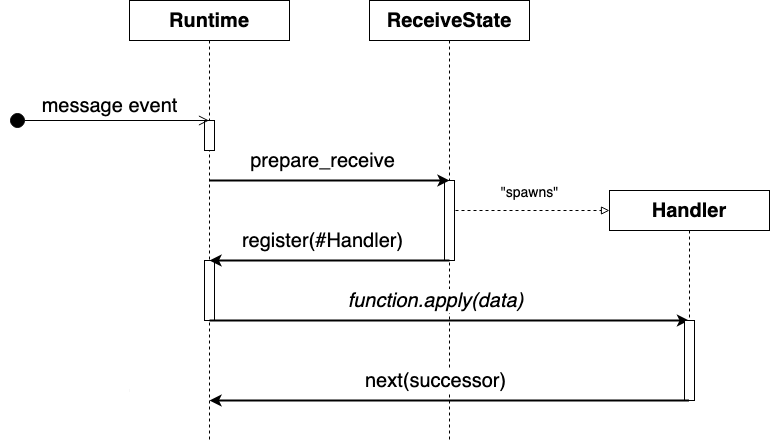
\includegraphics[width=\textwidth]{NodeRuntimeReceive1}
\caption{Message processed after transitioning to receive state}
\label{subfig:nodereceivehandlefirst}
\end{subfigure}
\caption{Possible Orderings for Receiving Message and
Registering Handler}
\label{fig:nodereceivecompare}
\end{figure}

We observe that defining the handler using an optional type
is insufficient. We need a similar mechanism for handling messages
waiting for handlers, and we cannot assume an ordering on the arrival
of messages that are not causally related.

We proceed to generalise our approach from one optional-type
handler to two mappings:
\textbf{(1)} a mapping from endpoint to message queues\footnote{
TypeScript arrays have built-in $O(1)$ time complexity
\texttt{shift()} and \texttt{push()} operations, which
can be used as a queue.}, and
\textbf{(2)} a mapping from endpoint to handler queues.
To simply put, if an incoming message is waiting for its handler,
it gets enqueued in the message queue labelled by the sender of the message;
when the handler is created, it pops the message off the queue 
and directly processes it; the same logic applies for a handler waiting
for its message.
We could have used a mapping from endpoint to optional type,
but queue operations elegantly hides the mechanics of
\cref{line:callhandlerstart,line:callhandler2,line:callhandler}
in \cref{lst:noderuntimewsmsg}.

We outline the changes made to the \texttt{Session} class,
as shown in \cref{lst:nodesession}:

\begin{enumerate}
\item We construct types for these two mappings 
(\cref{line:mapped1,,line:mapped2}), 
using a generic mapped typed defined below.
\begin{lstlisting}[language=javascript]
// Inside the Roles namespace...
export type PeersToMapped<Value> = { [Role in Peers]: Value };
\end{lstlisting}

\item Empty queues are initialised for both mappings
(\cref{line:queue1,,line:queue2}).

\item Each endpoint has a different \texttt{onmessage}
event listener, which will interact with the message queue
and handler queue corresponding to that endpoint. 
We achieve this by changing the \texttt{receive()} method
to be parameterised on the role instead 
(\cref{line:receivefunc}),
so it \textit{generates} an event listener 
(\cref{line:receivefuncret})
tailored for receiving messages
from that particular role.

\item
The \texttt{register()} method now also takes the role
as a parameter (\cref{line:newregister}) in order to check the 
corresponding pair of queues.
\end{enumerate}

\begin{figure}[!h]
\begin{lstlisting}[language=javascript,tabsize=2]
type RoleToMessageQueue = Roles.PeersToMapped<any[]>; (*@\label{line:mapped1}@*)
type RoleToHandlerQueue = Roles.PeersToMapped<MessageHandler[]>; (*@\label{line:mapped2}@*)
type RoleToSocket = Roles.PeersToMapped<WebSocket>;

class Session {
	...
	private roleToSocket: RoleToSocket;
	private messageQueue: RoleToMessageQueue;
	private handlerQueue: RoleToHandlerQueue;
	
	constructor(...) {
		...
		Object.values(Roles.Peers).forEach(role => {
			const socket = this.roleToSocket[role];
			socket.onmessage = this.receive(role).bind(this);
		});
		
		// Set up empty queues
		this.messageQueue = { [Roles.Peers.Client]: [], }; (*@\label{line:queue1}@*)
		this.handlerQueue = { [Roles.Peers.Client]: [], }; (*@\label{line:queue2}@*)
		
		this.next(initialState);		// Advance to initial state
	}
	
	receive(from: Roles) { (*@\label{line:receivefunc}@*)
	
		// Return a WebSocket message event listener
		// that looks at the message/handler queue
		// specific to the `from` role
		
		return ({ data }) => { (*@\label{line:receivefuncret}@*)
			// Array.shift() can return undefined if empty
			const handler = this.handlerQueue[from].shift();
			if (handler !== undefined) {
				handler(data);
			} else {
				this.messageQueue[from].push(data);			
			}
		}
	}
	
	register(from: Roles.Peers, handler: MessageHandler) { (*@\label{line:newregister}@*)
		const message = this.messageQueue[from].shift();
		if (message !== undefined) {
			handler(message);		
		} else {
			this.handlerQueue[from].push(data);		
		}
	}
}
\end{lstlisting}
\captionof{lstlisting}{Modified \texttt{Session} class to correctly
handle message receive events}
\label{lst:nodesession}
\end{figure}

Each endpoint must have consistency between
its message queue and handler queue.
We get the consistency from the simple fact that Node.js 
is a single-threaded runtime and execution is never pre-empted,
so there is no need to worry about atomic queue operations or
locking data structures.

We walk through how this design addresses the problems
in the previous example.

\begin{example}[Revisiting ``out-of-order'' message receives]
Consider the same multiparty session specified by the global type

\[
A \to S: \text{\lstonelinejs{M1(string)}}. 
B \to S: \text{\lstonelinejs{M2(number)}}. \texttt{end} 
\]

We show that our modified implementation addresses the problem:

\begin{enumerate}
\item 
\trole{S} transitions to its initial state,
``receive \lstonelinejs{M1(string)} from \trole{A}''.
\textit{The message queue for \trole{A} is empty,}
so the receive handler for \tmsg{M1} is registered 
\textit{under the handler queue for \trole{A}.}

\item
\tmsg{M2} arrives at \trole{S}, so the \texttt{onmessage}
handler is queued.

\item
\tmsg{M1} arrives at \trole{S}, so the \texttt{onmessage} handler
is queued.

\item
The \texttt{onmessage} handler for \tmsg{M2} is executed.
\textit{The handler queue for \trole{B} is empty, 
so \tmsg{M2} is added to the message queue for \trole{B}}.

\item
The \texttt{onmessage} handler for \tmsg{M1} is executed.
\textit{The handler queue for \trole{A} is non-empty,
so the handler is popped off the front of the queue 
and processes \tmsg{M1}.}

\item
\trole{S} transitions to the successor state, 
``receive \lstonelinejs{M2(number)} from \trole{B}''.
\textit{The message for \trole{B} is non-empty,
so \tmsg{M2} is popped off the queue and 
processed by the handler.}
\end{enumerate}

This execution is free of communication mismatches.
\end{example}

\subsection{Handling Termination}
WebSocket connections should be closed when the session terminates,
and both the browser endpoint and the server endpoint are capable
of closing connection. As we generate code for both, we define
a convention that the browser endpoint will close 
the WebSocket connection,
so we do nothing for this state at \cref{lst:noderuntime}.
\section{Alternative Designs}
\begin{itemize}
\item not sure whether to put this in the subsection above so it flows better?
\item naive implementation is to pass the send() function as a prop for the developer to incorporate in their event listener -- this is most flexible, but we cannot provide static guarantees
\item factory approach -- the runtime could pass a factory function which, takes an UI element and performs the binding; this is better, as channel resources are not exposed, but the adversarial-minded developer can later override the event listener in the DOM etc
\end{itemize}
\section{Limitations}
\label{section:nodelimitations}

Providing \textbf{static} communication safety guarantees have
come at a cost of providing relatively verbose APIs to the developer,
which introduces a learning curve. In particular,
the distinction between the \texttt{Implementation} and
\texttt{Handler} API should be an internal detail, but
the developer still needs to use the \texttt{Implementation} API
in their logic. 

Our APIs also rely on state identifiers, which also
does not help code readability, as it is neither apparent nor
self-documenting what \texttt{S51} refers to -- some existing work
\cite{Hybrid2016} augment the state identifiers with the channel
action and labels involved (e.g. 
\texttt{S51_Receive__Add_Number__Quit_String}).

Using handler-style APIs also mean that we require
nested scoping to propagate values between states,
which does not scale elegantly as the levels of nesting
increase. For example, the following implementation of
the \tprotocol{One Adder} protocol would be invalid if
we define the handlers for the continuations separately,
because the received payload are no longer in scope
(\cref{line:notinscope}).

\begin{lstlisting}[language=javascript]
const first = new S4({ NUM1: (x) => secondOperand, });
const second = new S6({ NUM2: (y) => sum, });
const sum = [Labels.S7.SUM, (*@\label{line:notinscope}\hl{???}@*), new S5()];
\end{lstlisting}

However, the developer may choose to propagate values
between states through persistent storage APIs (such as
storing values in a database and retrieving them for
handlers of continuation states), so our generated APIs
do not strictly enforce scoping to be the only way to
propagate values in the application logic.

\section{Summary}
In this chapter, we have presented
our session type API generation strategy
which targets the Node.js runtime for server-side
endpoints.

We motivated our approach of generating
handler-style APIs that act as seams in the session runtime
which executes the EFSM.
By doing so, the mechanism for sending and receiving
messages are not exposed to the developer,
which makes channel reuse impossible by construction.

We discussed our session runtime implementation in great
depth and iterated upon the design to arrive at 
a minimal runtime implementation that executes the EFSM
using a message-passing abstraction internally as well.
In particular, we motivated how to handle message receives
in a way that preserves the message ordering specified
in the communication protocol.

Developers that implement their Node.js endpoint application
using the generated APIs enjoy protocol conformance
by construction: 
the TypeScript type system will prevent type mismatches
in the handlers defined by the developer
(e.g. sending a \lstonelinejs{string} instead of 
a \lstonelinejs{number}, or using a message label
that is not defined on the EFSM state),
and the handler-style APIs themselves conceal channel
resources to prevent channel reuse.

\chapter{\fancyname{ReactMPST}: Front-End Session Type Web Development}

\section{Motivation}

\section{Approach}

\subsection{The React Framework}

\section{State Encodings}

\subsection{Send}

\subsection{Receive}

\subsection{Terminal}

\section{EFSM Execution Runtime}

\section{Alternative Designs and Limitations}

\section{Summary}

\chapter{Extensions}
\label{chap:ext}

In this chapter, we extend \codegen
to address concerns specific to modern web programming practices.
We focus on two key areas:
supporting asynchronous implementations (\cref{section:async}),
and handling session cancellation in a web-based context
(\cref{section:error}).

\section{Supporting Asynchronous Implementations}
\label{section:async}

Asynchronous APIs are commonplace in modern web programming,
ranging from database operations to third-party API calls.
We motivate the need for supporting asynchronous operations
through an authentication protocol in
\cref{subsection:asyncmotivation},
demonstrate how we support this through extending
the generated APIs and runtime in
\cref{subsection:asyncapi,subsection:asyncruntime}
respectively, 
and highlight the limitations of our approach in
\cref{subsection:asynclimit}.

\subsection{Motivation}
\label{subsection:asyncmotivation}

Consider a basic example of two-factor authentication 
(\tprotocol{2FA}) in \cref{lst:2FA} motivated from \cite{Exceptional}:
\trole{Client} tries to log in to \trole{Svr}, which either
authorises or denies the login attempt. If \trole{Client} is logging 
in from a new device, the \trole{Svr} sends a challenge key
and waits for a response code before proceeding.

\begin{figure}[!h]
\begin{lstlisting}[language=scribble]
global protocol 2FA(role Svr, role Client) {
	Login(string, string) from Client to Svr;
	choice at Svr { (*@\label{line:2fachoice1}@*)
		Authorised() from Svr to Client;
		do Main(Svr, Client);		// Details are not important
	} or {
		Challenge(string)	from Svr to Client;
		Response(number) 	from Client to Svr;
		choice at Svr { (*@\label{line:2fachoice2}@*)
			Authorised() from Svr to Client;
			do Main(Svr, Client);
		} or {
			AccessDenied() from Svr to Client;
		}
	} or {
		AccessDenied() from Svr to Client;	
	}
}
\end{lstlisting}
\captionof{lstlisting}{The \tprotocol{Two Factor Authentication} Protocol}
\label{lst:2FA}
\end{figure}

The developer's implementation on 
\cref{line:2fachoice1,line:2fachoice2} is likely to query
a database for credential verification.
Database operations are implemented using \textit{asynchronous},
\textit{non-blocking} APIs; it is
recommended that file operations do not block the main execution,
so a JavaScript database API may require a \textit{callback}
to propagate the return value when it is available.
A server endpoint implementation of \cref{lst:2FA}
may resemble the following:

\begin{lstlisting}[language=javascript]
new Implementation.S40({
	Login: (username: string, password: string) => {
		db.lookup(username, password, (result) => {
			// returns Implementation.S42 here
		});
	}
});
\end{lstlisting}

Callbacks are commonplace in dealing with concurrency in JavaScript
\cite{CallbackHell}; we will go over other widely-used
concurrency primitives shortly.
Whatever the case may be, asynchronous developer implementations
using our generated APIs will not type-check as the function
returns immediately (hence, has return type \lstonelinejs{void}),
even though the callback function has the expected return type.
The developer will encounter the following:

\begin{lstlisting}[tabsize=2,numbers=none]
Type '(username: string, password: string) => void' is not 
assignable to type '(payload_0: string, payload_1: string) => S42'.
\end{lstlisting}

This is also possible for browser-side implementations:
when the user invokes a UI event, the browser-side logic
may first consult a third-party API for additional information
(which is not part of the communication protocol)
before performing a send action; the \textit{Fetch} API \cite{Fetch}
for making API calls is asynchronous.

In order to make \fancyname{SessionTS} more relevant and compatible
with modern web programming practices, it is important to
support asynchronous developer implementations as part of our
generated APIs and runtime. 

This means we should support
the concurrency primitives built into TypeScript:

\subparagraph{Callbacks}
Callback-based APIs are higher-order functions -- they take functions
as parameters and invoke them when the asynchronous operation is complete.
The \texttt{setTimeout(fn, delay)} function available on the browser
waits for \texttt{delay} milliseconds before invoking \texttt{fn()} --
or more precisely, before queuing the execution of \texttt{fn()}.
As a result, the code listing below prints \lstonelinejs{'Second!'}
before \lstonelinejs{'First!'}, even though \texttt{setTimeout}
was called with 0ms delay.

\begin{lstlisting}[language=javascript,numbers=none]
setTimeout(() => console.log('First!', 0);
console.log('Second!');
\end{lstlisting}

\subparagraph{Promises}
A Promise formalises the ``completion'' callback
and its error handling construct. The developer passes a ``success''
handler and ``error'' handler, conventionally named
``then'' and ``catch'' respectively, to construct a Promise.
This is analogue to the \texttt{Future} interface in Java \cite{JavaFuture}.
The Promise will invoke the correct handler on completion.
The benefits of Promises in our context is that TypeScript allows
us to specify the type of payload that the Promise resolves to.

\begin{lstlisting}[language=javascript,numbers=none]
declare function promise(n: number): Promise<number>
const promise = (n: number) => 
	new Promise((resolve, reject) => {
		if (n < 10)  resolve(n));
		else reject('Number too big!');
	});

declare function handleNumber(n: number) { ... } 
declare function handleError(err: string) { ... }

promise(10).then(handleNumber).catch(handleError)
\end{lstlisting}

\subparagraph{Async/Await}
The \lstonelinejs{async}/\lstonelinejs{await} construct
is syntactic sugar for Promises. An \lstonelinejs{async}
function always returns a Promise, and marking \lstonelinejs{await}
for the identifier of the return value for a function returning a Promise
``unwraps'' the resolved payload. A downside is that error handling
reverts to the \lstonelinejs{try ... catch} construct.

\begin{lstlisting}[language=javascript,numbers=none]
const asyncSum = async (x: number, y: number) => {
	return (await promise(x)) + (await promise(y));
}

asyncSum(1, 2);  // returns Promise<number> that resolves to 3
\end{lstlisting}

\subsection{API Extension}
\label{subsection:asyncapi}

This is rather straightforward.
We construct a generic union type, \texttt{MaybePromise<T>},
to specify that the type parameter might be wrapped in a Promise,
and leverage type inference in conditional types to
define a generic type, \texttt{FromPromise<T>}, to extract
the wrapped type.

\begin{lstlisting}[language=javascript,numbers=none]
type MaybePromise<T> = T | Promise<T>;
type FromPromise<T> = T extends MaybePromise<infer R> ? R : never;
\end{lstlisting}

Now we change the type signatures of our generated APIs
to use \texttt{MaybePromise<T>}.
For example, if the handler of a receive state generated by
\fancyname{NodeMPST} must return \texttt{Implementation.S42},
it is now permitted to return a \texttt{Promise} that resolves
to a value of type texttt{Implementation.S42}.
The same logic applies to other types of EFSM states
in both \fancyname{NodeMPST} and \fancyname{ReactMPST}.

Hence, the asynchronous \trole{Svr} implementation
for the 2FA protocol shown in \cref{lst:new2fa}
now type-checks. Note that, because 
\lstonelinejs{async} functions return \texttt{Promise}s,
we also support this newer piece of syntactic sugar.

\begin{figure}[!h]
\begin{lstlisting}[language=javascript,tabsize=2]
new Implementation.S40({
	Login: (*@\hl{async}@*) (username: string, password: string) => {
		const result = (*@\hl{await}@*) db.lookup(username, password);
		if (result.valid)
			return new Implementation.S42('Authorised', ...);
		else if (result.unauthorised)
			return new Implementation.S42('AccessDenied', ...);
		else
			return new Implementation.S42('Challenge', ..., challenger);
	}
});

const challenger = (key: number) => {
	return new (*@\hl{Promise}@*)((resolve, reject) => {
		keychain.check(key, ok => {
			if (ok)
				resolve(new Implementation.S44('Authorised', ...);
			else 
				resolve(new Implementation.S44('AccessDenied', ...);	
		});
	});
}
\end{lstlisting}
\captionof{lstlisting}{\tprotocol{2FA} \trole{Svr} Implementation using 
Callbacks, \texttt{Promise}s and
\lstonelinejs{async}/\lstonelinejs{await}}
\label{lst:new2fa}
\end{figure}

\subsection{Runtime Extension}
\label{subsection:asyncruntime}

Generally, minimal changes are required for the runtime.
The key observation is that the concrete types for the any
handlers are the same -- they just might be wrapped in a Promise
construct.
To handle potential Promises, we wrap existing logic
as a delayed computation, colloquially known as a \textit{thunk}
\cite{Thunk}.
We show an example in \cref{fig:thunk} of how we
adapt the \texttt{performSend()} function generated by
\fancyname{NodeMPST} to support optional \texttt{Promise}s:

\begin{enumerate}
\item
We wrap the original logic in \cref{subfig:originalthunk} into a
function (\cref{subfig:newthunk} \cref{line:thunk})
to delay the computation.

\item
We distinguish asynchronous implementations
from synchronous ones using the \lstonelinejs{instanceof} operator.

\begin{itemize}
\item
If the implementation is a \texttt{Promise}, we pass
the thunk as the resolve function invoked on completion.

\item
Otherwise, we directly invoke the computation.
\end{itemize}

\end{enumerate}

\begin{figure}[!h]
\begin{subfigure}{\textwidth}
\begin{lstlisting}[language=javascript,tabsize=2]
const [label, payload, succ] = this.handler;
send(label, payload);
next(succ);
\end{lstlisting}
\caption{Original \texttt{performSend()} Implementation}
\label{subfig:originalthunk}
\end{subfigure}
\hfill
\begin{subfigure}{\textwidth}
\begin{lstlisting}[language=javascript,tabsize=2]
const thunk = (label, payload, succ) => { (*@\label{line:thunk}@*)
	send(label, payload);
	next(succ);	
};

if (this.handler instanceof Promise)
	this.handler.then(thunk);
else
	thunk(this.handler);
\end{lstlisting}
\caption{New \texttt{performSend()} for Optional \texttt{Promise}s}
\label{subfig:newthunk}
\end{subfigure}
\caption{Adapting Send Operations in \fancyname{NodeMPST}
using a Thunk}
\label{fig:thunk}
\end{figure}

Similar changes apply to other types of states in both
\fancyname{NodeMPST} and \fancyname{ReactMPST}.
For \fancyname{ReactMPST}, channel-related functions in the runtime
return the successor state identifier. Hence, aside from
refactoring the functions to delay computation using thunks,
the functions themselves need to
return \texttt{MaybePromise<State>} instead
to propagate the asynchrony
to the execution of the EFSM -- the transition occurs
\textit{after} the developer's handler finishes execution.

\subsection{Limitations}
\label{subsection:asynclimit}

Supporting asynchronous logic on top of our
existing implementation in \fancyname{ReactMPST} comes at a cost
of losing affine linearity guarantees.
If the send action handler is asynchronous, then the UI event handler
returns before the runtime transitions, so the UI event that can trigger
the send action is still active, which means the user can trigger
a channel linearity violation. This means we need a boolean flag
to keep track of channel usage, as done in \cite{Hybrid2016}.
We illustrate this in \cref{lst:asynclinearcheck},
with the linearity checks highlighted.

\begin{figure}[!h]
\begin{lstlisting}[language=javascript,tabsize=2]
(*@\hl{let used = false;}@*)
...
return class extends React.Component {
	render() {
		const props = {
			[eventLabel as string]: (event) => {
				(*@\hl{if (used) return;}@*)
				(*@\hl{used = true;}@*)
				
				const result = handler(event);
				if (result instanceof Promise)
					result.then(send);
				else
					send(result);
			}		
		}
	}
}
\end{lstlisting}
\captionof{lstlisting}{\dots}
\label{lst:asynclinearcheck}
\end{figure}

If we decouple the \texttt{sendMessage()} 
from the \texttt{advance()} function, we could advance to the successor state
immediately \textit{before} handling the asynchronous return value.
This restores affine channel linearity guarantees, but 
results in the UI being inconsistent with the channel
actions.

\section{Error Handling}
\label{section:error}

A robust error handling framework is critical
in a distributed setting.
It is naive to assume that endpoint implementations
are entirely free from exceptions.
As Fowler pointed out in \cite{Exceptional},
session type implementations that do not account for failure
are of limited use in distributed programming.

We motivate the need for handling a variety exceptions in
modern web programming in \cref{subsection:errormotivation},
demonstrate how we implement a structured error handling
framework through extending the generated APIs and 
runtime in \cref{subsection:errorapi,subsection:errorruntime}
respectively, and explain the limitations of our framework
in \cref{subsection:errorlimit}.

\subsection{Motivation}
\label{subsection:errormotivation}

Using the \tprotocol{2FA} example from
\cref{lst:2FA}, the database lookup function
might rely on a cloud service, and will throw an exception
if the cloud service cannot be reached.
This may cause \trole{Svr} to crash.
From the perspective of session types, we need to
ensure that \trole{Client} isn't blindly
waiting for the session to continue if \trole{Svr}
threw an exception.

We classify this as an example where \trole{Svr}
terminates the session because of a \textit{logical error}
in its implementation.
Existing work \cite{Exceptional,AffineSessions} 
on error handling for session types address this
through extending the process calculus with an
\textit{explicit cancellation} operator to ensure that
channel resources are closed during exception handling.

However, the context of modern web programming
introduces new possibilities for session cancellation
that are not addressed by existing work.
Browser-side endpoints can disconnect from the session due
to network connectivity issues or simply by closing
the browser. Similarly, the server may also face connectivity
issues. In order to deliver a robust error handling
framework tailored for integrating session types in 
modern web programming, we must also take these variants
of session cancellation into account.

We also need a novel approach for defining cancellation handlers.
The work by Fowler et al. \cite{Exceptional} integrates 
exception handling for session types in a 
\textit{functional language}, where their design of
exception handlers build upon existing work on effect handlers.
Our work targets a non-functional language in TypeScript,
which means any piece of code can be ``effectful'',
so the exception handler API we generate for developers
need to respect this property.
Exception handlers should also be well parameterised
to empower the developer to handle cancellations more effectively
-- for instance, if the developer knows which endpoint
emitted the cancellation, appropriate clean-up operations
(such as reverting database changes or application-specific
logging) can be performed.

\subsection{API Extension}
\label{subsection:errorapi}

\begin{itemize}
\item developers just need to provide cancellation handlers along with the initial state
\item we standardise on parameterising it with role and reason: the reason is typed `any' to give developers the autonomy for implementation details
\end{itemize}

\begin{figure}[!h]
\begin{lstlisting}[language=javascript]
new ATMSvr(wss, logic, async (role: Roles.All, reason: any) => {
	if (role === Roles.Self) {
		// Handle internal server error	
	} else {
		// Handle client error:
		// revert incomplete transactions from database
		await db.revertTransactions(role);
	}
});
\end{lstlisting}
\captionof{lstlisting}{Example Cancellation Handler for Server Endpoint}
\label{lst:cancelsvr}
\end{figure}

\begin{figure}[!h]
\begin{lstlisting}[language=javascript]
<ATMClient
	endpoint='ws://localhost:8080'
	...
	cancellation={(role: Roles.All, reason: any) => (
		<div>
			{role === Roles.Self
				? <h1>Internal Error</h1>
				: <h1>Server Error</h1>}
			<p>{reason}</p>
		</div>
	)}	
/>
\end{lstlisting}
\captionof{lstlisting}{Example Cancellation Handler for Browser Endpoint}
\label{lst:cancelclient}
\end{figure}

\subsection{Runtime Extension}
\label{subsection:errorruntime}

The generated session runtime \dots

\begin{itemize}
\item build upon websocket RFC which specifies the `base' closing (or exit) code
\item we additionally define contracts for exit codes in our use case (e.g. role occupied, logical error), and make sure it does not override any websocket `traditions' as per the RFC
\item all based on well-defined event listeners on the websocket close and error events
\item must consider cancellation in two phases
\end{itemize}

\subsubsection{Cancellations during Session Joining}

\begin{itemize}
\item server -- emits role occupied
\item client -- closes browser whilst waiting for others
\end{itemize}

\subsubsection{Cancellations during EFSM Execution}

\begin{itemize}
\item server -- dies
\item server -- logical error
\item client -- dies
\item client -- logical error
\end{itemize}

\subsection{Limitations}
\label{subsection:errorlimit}

The expressiveness of our error handling framework is
limited by the expressiveness of the 
\lstonelinejs{try} / \lstonelinejs{catch} mechanism
in TypeScript.

\begin{itemize}
\item Cancellation handlers are not typed -- namely, we use `any';
\item exception handler blocks in typescript are not typed
\item the `logical error' idea is also very vague as all code can be effectful in typescript (statically); cannot specifically say that the implementation is expected to `send payload of type int, but possibly throw error of type Error', which would otherwise be possible in other languages(?)
\end{itemize}


\part{Implementing Arbitrary Topologies over WebSockets}
\label{part:general}

\chapter{Motivation: Supporting Peer-to-Peer Interactions}
\label{chap:p2p}

\section{\fancyname{Two Buyer} Protocol}

We present the \tprotocol{Two Buyer} protocol in \cref{lst:twobuyer}.

\begin{figure}[!ht]
\begin{lstlisting}[language=Scribble, tabsize=2]
module ClientClient;

global protocol TwoBuyer(role A, role B, role S) {
	title(string)      from A to S;
	quote(number)      from S to A;
	quote(number)      from S to B;
	quoteByTwo(number) from A to B;
	choice at B {
		ok()           from B to S;
		date(string)   from S to B;
	} or {
		quit()         from B to S;
	}
}
\end{lstlisting}
\captionof{lstlisting}{The \tprotocol{Two Buyer} Protocol}
\label{lst:twobuyer}
\end{figure}

Assume \trole{S} is the server, and roles \trole{A}, \trole{B} run on the 
browser:

\begin{enumerate}
\item \trole{A} sends to \trole{S} the title of an item to sell;
\item \trole{S} sends a quote for said item to \trole{A} and \trole{B};
\item \trole{A} privately sends a separate quote to \trole{B};
\item \trole{B} makes a choice:
\begin{itemize}
\item if \trole{B} prefers the offer from \trole{S}, 
\trole{B} replies \tmsg{ok()} to \trole{S}, and \trole{S} informs
\trole{B} of the delivery date;

\item otherwise, \trole{B} takes the offer from \trole{A} and simply
responds \tmsg{quit()} to \trole{S}.
\end{itemize} 
\end{enumerate}

\begin{itemize}
\item TwoBuyer example -- highlight the sections that show the `arbitrary topology'
\item Not possible with WebSocket topology
\end{itemize}


\section{Server as a Router}
\begin{itemize}
\item How to make TwoBuyer example work just with WebSockets
\item Quickly highlight WebRtC as an option, but it has its own proprietary connection `protocol', and will still need to rely on a centralised server role to set up the peer to peer connection; including the setup in the code generation will introduce unnecessary complications in error handling which deviates from the focus of implementing typesafe web services
\item Essentially `decomposing' multiparty session into binary interactions with respect to the server
\end{itemize}

\section{Challenges}
\begin{itemize}
\item Routed communication is different from `normal' communication
- server cannot overserialise interactions
\item Existing work in decomposing multiparty sessions (see LinearDecompScala paper and the binary one it references) assume the `server' takes on the pure role as a router -- our work argues that the server can still participate in the multiparty session and concurrently route messages between clients in a way that does not overserialise the interactions and allow the routing to be transparent to other roles.
\item theory side -- need to prove that it is indeed possible for the server to carry out its own interactions and perform routing in a transparent way, as if the messages were directly peer to peer
\item implementation side -- changes need to reflect the theory and be as transparent to the developer as possible
\end{itemize}

\chapter{Theory: Routed Session Types}

\section{Syntax}

\subsection{Global Types}

\subsection{Local Types}

\section{Labelled Transition System (LTS) Semantics}

\subsection{Trace Equivalence}

\subsection{Deadlock Freedom}

\section{Router-Parameterised Encoding}

\subsection{Preserving Well-formedness}

\subsection{Preserving Communication}

\section{Implementation}

\codegen is written in Python. 
It offers flexible syntax, a rich standard library, and 
a healthy ecosystem of DOT graph parsers and template engines,
making it a suitable choice for implementing our code generator.
Its rich standard library also simplifies many tasks: we use
the \texttt{argparse} package to generate an informative
command line interface (CLI) for developers to 
supply the correct information (\cref{lst:cmdline})
to use \codegen
and the \texttt{subprocess} package to 
invoke external tools, such as Scribble and the TypeScript Compiler.

\begin{figure}[!ht]
\begin{lstlisting}
root@mpst_ts:/home# python3.7 -m mpst_ts --help
usage: __main__.py [-h] [-s SERVER] [-o OUTPUT]
                   filename protocol role {browser,node}

positional arguments:
  filename       Path to Scribble protocol
  protocol       Name of protocol
  role           Role to project
  {browser,node} Code generation target

optional arguments:
  -h, --help     show this help message and exit
  -s SERVER, --server SERVER
                 Server role (only applicable for browser targets)
  -o OUTPUT, --output OUTPUT
                 Output directory for generation
\end{lstlisting}
\captionof{lstlisting}{Entry Point for \codegen}
\label{lst:cmdline}
\end{figure}

We use Docker \cite{docker} to encapsulate our code generator
and its dependencies -- 
we found the canonical Python virtual environment
solution to be insufficient, as the Scribble toolchain is
a standalone Java executable with non-trivial setup procedures.
The Dockerfile builds a Docker image with Scribble and
the Python dependencies all pre-configured, and the provided
\texttt{build.sh} script instantiates the image as a container 
for development.
The \texttt{start.sh} script enters the Docker container
development environment and mounts the local project directory
onto the container as a volume to synchronise changes between the
two environments.

\part{Evaluation and Conclusion}

\chapter{Evaluation}
\label{chap:eval}
%benchmark -- compile time / benchmarking 

\section{Binary Sessions: \fancyname{Calculator}}
\begin{itemize}
\item sample client implementation + snippet of generated code (full in appendix)
\item show that not all the UI is being controlled by the runtime (i.e. calculator app has a header/fake navbar)
\item show the calculator logic achievable using React Context
\item sample server implementation + snippet of generated code (full in appendix)
\end{itemize}

\section{Multiparty Sessions: \fancyname{Noughts and Crosses}}
\begin{itemize}
\item sample client implementation -- show the flexibility of factory API for sending to be used in the UI part (since move selection can be be made )
\end{itemize}

\section{Routed Multiparty Sessions: \fancyname{Two Buyers}}
\begin{itemize}
\item show that the routing aspect is transparent to both sides
\end{itemize}

\section{Performance Benchmarks}

Whilst web applications that implement our generated APIs enjoy
communication safety guarantees, the presence of the session runtime acts
as an additional layer of abstraction between the application logic and the
WebSocket transport, which is likely to present a performance trade-off.

To measure the overhead of our implementation, we compare the
execution time of an interactive web application implementing the
Ping Pong protocol (\cref{fig:pingpong}) using our generated APIs
against an implementation of the protocol without session types.

We standardise the application logic across experiments to be 
parameterised by the number of round trip messages, $n$.
Upon establishing a connection, the experiment proceeds as follow:

\begin{enumerate}

\item \trole{Client} sends a \tmsg{PING($m$:number)} message, 
with $m = 0$ initially.

\item \trole{Server} receives the \tmsg{PING($m$:number)} message, and
conditionally responds based on the experiment parameter $n$:

\begin{enumerate}
\item If $m + 1 < n$, then \trole{Server} responds with \tmsg{PONG($m + 1$)}.
\trole{Client} responds to the \tmsg{PONG} message by returning to
step 1 with $m$ set as the payload of the received \tmsg{PONG} message.

\item Otherwise, $m + 1 = n$, then \trole{Server} responds with 
\tmsg{BYE($m + 1$)}, as $n$ round trips have taken place. 
\trole{Client} responds to the
\tmsg{BYE} message by closing the connection, thus ending the experiment.
\end{enumerate}

\end{enumerate}

%\begin{itemize}
%\item compile time: \begin{itemize}
%\item use the examples from above to compare compilation time
%\end{itemize}
%\item execution time: based on parameterised ping pong with n messages
%\begin{itemize}
%\item n = 10, 100, 1000
%\item benchmark using node timer tools in the backend as it knows when the protocol ends
%\end{itemize}
%\end{itemize}

\subsection{Setup}

% mention that it is hard to simulate multi-party sessions 
% and see the overhead with increasing roles (eg ping pong with 50 roles)
% , because of the need to
% mock developer implementations for those roles

We run the experiments under a network of latency 0.165ms
(64 bytes ping), and repeat each experiment 20 times.
Compilation time and execution time measurements 
are taken using a machine equipped with Intel i7-4850HQ CPU
(2.3 GHz, 4 cores, 8 threads), 16 GB RAM, macOS operating system 
version 10.15.4, Node.js runtime version 12.12.0, and
TypeScript compiler version 3.7.4.

The other packages used in all implementations are outlined in their
corresponding \texttt{package.json} files.

\paragraph{\fancyname{Bare} variant}
\dots

\paragraph{\fancyname{BareSafe} variant}
\dots

\paragraph{\fancyname{MPST} variant}
\dots

\subsection{Execution Pattern}

\subsection{Analysing Overhead}

\chapter{Conclusion}
\label{chap:concl}

\section{Contributions}

In this project, we develop and present an
MPST-based framework for developing full-stack
interactive TypeScript applications over WebSocket transport.

We motivate our API generation approach from 
\cite{Hybrid2016,PureScript2019} to generate TypeScript APIs
from a Scribble protocol specification.
Developers write their full-stack applications
by implementing the generated APIs, and can enjoy 
communication safety guarantees by construction.
We explain how our session type encodings target the Node.js
server-side runtime and React.js framework in
\cref{chap:node,chap:react} for server-side
and browser-side endpoints respectively.

In particular, we present a novel approach for integrating
session types into web-based GUI programming based on
translating the theory on model types \cite{MVU2020}
to idiomatic practices on the React.js framework.
With respect to session type theory, implementations using
the generated APIs statically enjoy linear channel usage
guarantees and affine channel usage guarantees for back-end
and front-end targets respectively.

Compared to previous work, we are not only able to
\textbf{statically} provide the same level of communication safety
guarantees from multiparty session type theory, but we do so
using modern web programming practices to increase
the relevance and usability of our work in industry:
our work targets TypeScript, Node.js and React.js,
and we explain in \cref{chap:ext} how we support advanced
web development idioms such as asynchronous implementations.

In addition, existing proposals on API generation for web development
over WebSockets \cite{PureScript2019} only support protocols
implementing server-centric topologies, in order to be 
compatible with WebSocket transport.
We formalise a theory of routed multiparty session types in 
\cref{chap:theory} to prove that it is possible to relax the
server-centric topology assumption over WebSocket transport in a way 
that preserves communication along with the communication safety 
properties inherited from canonical session type theory.

% PLACES
Our work has received positive feedback from academia.
The project has been accepted and published as 
\emph{Generating Interactive WebSocket Applications in TypeScript}
in Volume 314 of the Electronic Proceedings in Theoretical
Computer Science \cite{PLACES2020}; we were also invited to present this work
at the 12th International Workshop on
Programming Language Approaches to Concurrency- \& 
Communication-cEntric Software (PLACES 2020).

% OVERALL
Overall, we offer an end-to-end solution for integrating
multiparty session type theory into modern full-stack web programming
practices, in a way that actively encourages developers to
design their application with communication safety in mind.
Our formalism of routed multiparty session types enables our
API generation tool to support a wider range of protocols, and
further reveals the potential
for implementing dynamic communication structures over centralised
network topologies.

\section{Future Work}
\label{section:future}

We highlight several areas of future work
to support a wider range of communication protocols
for web applications and increase the 
industrial relevance of our work.

\paragraph{Session Delegation}
Delegation allows channels to be sent between endpoints.
Using the \tprotocol{Noughts and Crosses} game
from \cref{section:evalgame}, the developer
may want the \trole{Svr} to send a private channel
to both players to play the game,
whilst concurrently accepting new connections.

The API generation solution 
presented by Scalas et al. \cite{LinearDecomp} supports
\textit{distributed multiparty delegation} in Scala.
Their work also uses the Scribble toolchain
for protocol specification.
Future work can apply the findings from \cite{LinearDecomp}
and extend \codegen to support channel delegation
in the generated handler-style APIs.

\paragraph{Explicit Connection Actions}
Hu and Yoshida \cite{ExplicitConnections} extended 
MPST theory
with \textit{explicit connection actions} to support protocols 
with optional participants.
Supporting optional participants is a relevant concept
for web applications, particularly for browser-side endpoints.

Our work defines a way to handle connection requests
and detect disconnection events. The implementation assumes that
all participants join the session when the protocol begins.
We also focus on disconnection events as a result of session
cancellation rather than those stated in the protocol.

\cite{ExplicitConnections} uses a variant of the Scribble protocol
language that supports explicit connection actions. Future work
can use that as a basis for code generation, and generalise
our existing mechanisms for session connection and cancellation
to support explicit connection actions.

\paragraph{Transport Abstraction}
The MPST-based web development framework presented by 
King et al. \cite{PureScript2019} parameterises
the transport mechanism in the session runtime definition.
The developer can run the session over different transportation,
provided that the custom transport implements the behaviour
of the \texttt{Transport} type class.

Future work can generalise the session runtime for 
\fancyname{NodeMPST} and \fancyname{ReactMPST} to provide
similar abstractions. A successful implementation could
possibly allow direct interactions between two Node.js-based
endpoints, but this will also require the routed MPST
theory to be adapted accordingly to reason about
such interactions in a web-based context.

\paragraph{EFSM Encoding as Typestates}
The concept of \textit{typestates} define the interface of
an object to be dependent on its private state, meaning
it can change at runtime.
This is compatible with the EFSM abstraction from the
MPST framework: the permitted methods (i.e. channel actions)
of the EFSM depends on its current state.
In fact, Kouzapas et al. \cite{StMungo} presents a way to
generate typestate specifications for each endpoint of a
Scribble protocol; Gay et al. \cite{ModularST} proposes
an encoding of session types in object-oriented languages
and discuss their approach with respect to typestates.

Future work can explore implementing typestates
in TypeScript. A linear type system would be useful towards 
implementing typestates, but this is lacking in TypeScript.
One interesting possibility for approximating this would
be to combine \textit{decorators} with \textit{transformers}:
the former lets the developer define typestate-related metadata,
whilst the latter can parse the metadata and
transform the source code into another TypeScript program that acts
as an ``intermediate representation'',
such that only implementations that respect the typestate specification
will type-check with its intermediate representation.



\clearpage
\bookmarksetup{startatroot}

\bibliographystyle{acm}
\bibliography{report}

\appendix
\chapter{Lemmas and Proofs for \cref{chap:theory}}

\chapter{Evaluation}
\label{chap:eval}
%benchmark -- compile time / benchmarking 

\section{Binary Sessions: \fancyname{Calculator}}
\begin{itemize}
\item sample client implementation + snippet of generated code (full in appendix)
\item show that not all the UI is being controlled by the runtime (i.e. calculator app has a header/fake navbar)
\item show the calculator logic achievable using React Context
\item sample server implementation + snippet of generated code (full in appendix)
\end{itemize}

\section{Multiparty Sessions: \fancyname{Noughts and Crosses}}
\begin{itemize}
\item sample client implementation -- show the flexibility of factory API for sending to be used in the UI part (since move selection can be be made )
\end{itemize}

\section{Routed Multiparty Sessions: \fancyname{Two Buyers}}
\begin{itemize}
\item show that the routing aspect is transparent to both sides
\end{itemize}

\section{Performance Benchmarks}

Whilst web applications that implement our generated APIs enjoy
communication safety guarantees, the presence of the session runtime acts
as an additional layer of abstraction between the application logic and the
WebSocket transport, which is likely to present a performance trade-off.

To measure the overhead of our implementation, we compare the
execution time of an interactive web application implementing the
Ping Pong protocol (\cref{fig:pingpong}) using our generated APIs
against an implementation of the protocol without session types.

We standardise the application logic across experiments to be 
parameterised by the number of round trip messages, $n$.
Upon establishing a connection, the experiment proceeds as follow:

\begin{enumerate}

\item \trole{Client} sends a \tmsg{PING($m$:number)} message, 
with $m = 0$ initially.

\item \trole{Server} receives the \tmsg{PING($m$:number)} message, and
conditionally responds based on the experiment parameter $n$:

\begin{enumerate}
\item If $m + 1 < n$, then \trole{Server} responds with \tmsg{PONG($m + 1$)}.
\trole{Client} responds to the \tmsg{PONG} message by returning to
step 1 with $m$ set as the payload of the received \tmsg{PONG} message.

\item Otherwise, $m + 1 = n$, then \trole{Server} responds with 
\tmsg{BYE($m + 1$)}, as $n$ round trips have taken place. 
\trole{Client} responds to the
\tmsg{BYE} message by closing the connection, thus ending the experiment.
\end{enumerate}

\end{enumerate}

%\begin{itemize}
%\item compile time: \begin{itemize}
%\item use the examples from above to compare compilation time
%\end{itemize}
%\item execution time: based on parameterised ping pong with n messages
%\begin{itemize}
%\item n = 10, 100, 1000
%\item benchmark using node timer tools in the backend as it knows when the protocol ends
%\end{itemize}
%\end{itemize}

\subsection{Setup}

% mention that it is hard to simulate multi-party sessions 
% and see the overhead with increasing roles (eg ping pong with 50 roles)
% , because of the need to
% mock developer implementations for those roles

We run the experiments under a network of latency 0.165ms
(64 bytes ping), and repeat each experiment 20 times.
Compilation time and execution time measurements 
are taken using a machine equipped with Intel i7-4850HQ CPU
(2.3 GHz, 4 cores, 8 threads), 16 GB RAM, macOS operating system 
version 10.15.4, Node.js runtime version 12.12.0, and
TypeScript compiler version 3.7.4.

The other packages used in all implementations are outlined in their
corresponding \texttt{package.json} files.

\paragraph{\fancyname{Bare} variant}
\dots

\paragraph{\fancyname{BareSafe} variant}
\dots

\paragraph{\fancyname{MPST} variant}
\dots

\subsection{Execution Pattern}

\subsection{Analysing Overhead}


\end{document}
%%% Local Variables: 
%%% mode: latex
%%% TeX-master: t
%%% End: 
